\documentclass[
a5paper,
%paper=5.5in:8.5in,
]{scrbook} 


\title{A Little Princess}

\usepackage[namedChapters]{bindery}
\usepackage{dropcaps}



\setdropcaps{FloralCapitals.ttf}
\setotherlanguage{french}


\begin{document}
\frontmatter

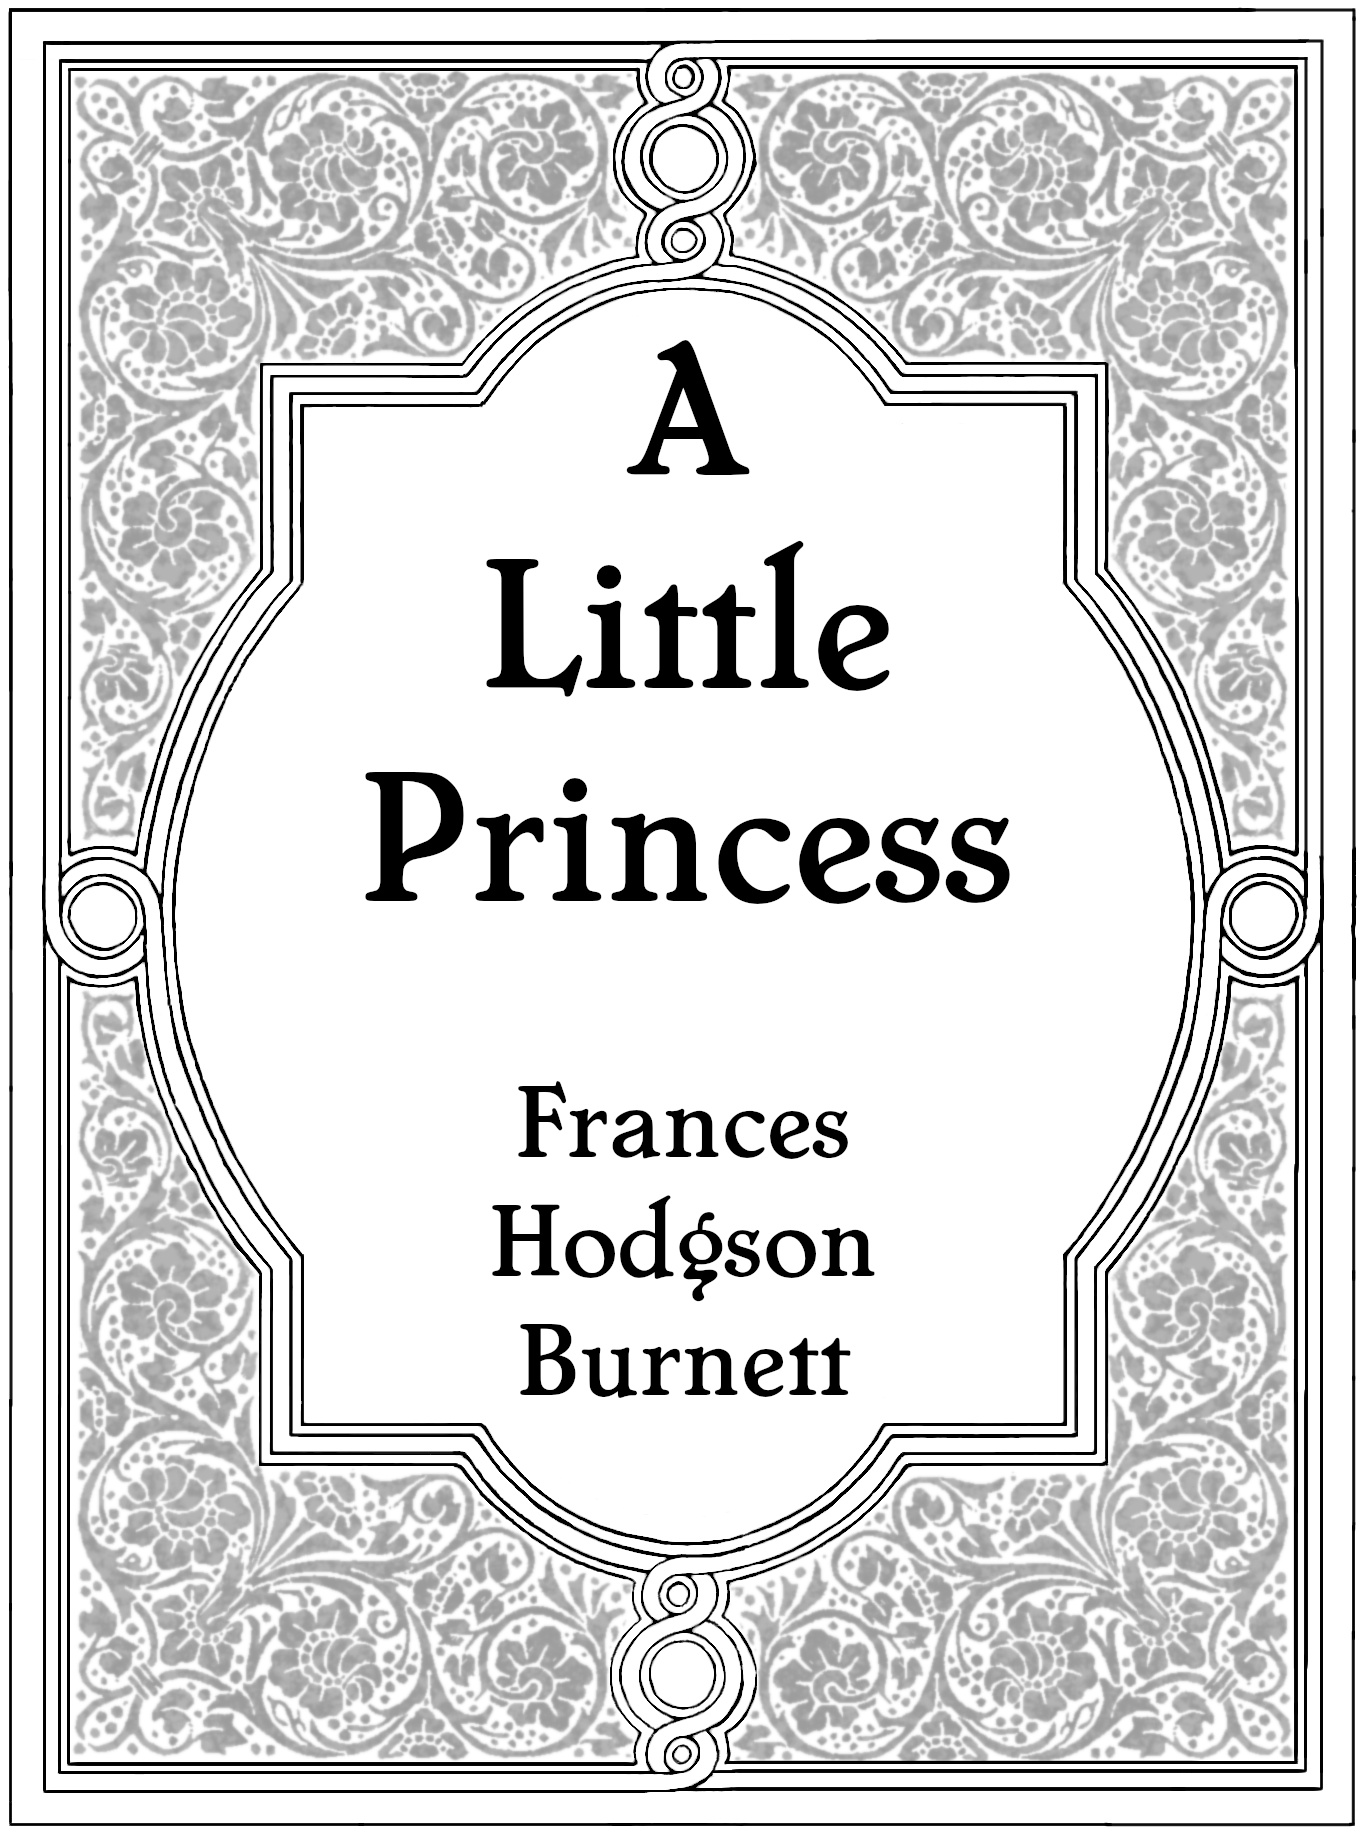
\includepdf[width=1.3\textwidth]{titlepage.jpg}
 


\pagestyle{plain}




\tableofcontents
\clearpage




\renewcommand*{\chapterpagestyle}{plain}

\KOMAoptions{headings=openright}


 
 \mainmatter
  \renewcommand*{\chapterheadstartvskip}{\vspace{0pt}}
 \pagestyle{headings}
%!TeX root=../princesstop.tex
\chapter{Sara}
\begin{figure}[t!]
\centering

\includegraphics[width=\linewidth]{filigree}
\end{figure}
\lettrine[lines=5]{O}{nce} on a dark winter's day, when the yellow fog hung so thick and heavy in the streets of London that the lamps were lighted and the shop windows blazed with gas as they do at night, an odd-looking little girl sat in a cab with her father and was driven rather slowly through the big thoroughfares.

She sat with her feet tucked under her, and leaned against her father, who held her in his arm, as she stared out of the window at the passing people with a queer old-fashioned thoughtfulness in her big eyes.

She was such a little girl that one did not expect to see such a look on her small face. It would have been an old look for a child of twelve, and Sara Crewe was only seven. The fact was, however, that she was always dreaming and thinking odd things and could not herself remember any time when she had not been thinking things about grown-up people and the world they belonged to. She felt as if she had lived a long, long time.

At this moment she was remembering the voyage she had just made from Bombay with her father, Captain Crewe. She was thinking of the big ship, of the Lascars passing silently to and fro on it, of the children playing about on the hot deck, and of some young officers' wives who used to try to make her talk to them and laugh at the things she said.

Principally, she was thinking of what a queer thing it was that at one time one was in India in the blazing sun, and then in the middle of the ocean, and then driving in a strange vehicle through strange streets where the day was as dark as the night. She found this so puzzling that she moved closer to her father.

»Papa,« she said in a low, mysterious little voice which was almost a whisper, »papa.«

»What is it, darling?« Captain Crewe answered, holding her closer and looking down into her face. »What is Sara thinking of?«

»Is this the place?« Sara whispered, cuddling still closer to him. »Is it, papa?«

»Yes, little Sara, it is. We have reached it at last.« And though she was only seven years old, she knew that he felt sad when he said it.

It seemed to her many years since he had begun to prepare her mind for »the place,« as she always called it. Her mother had died when she was born, so she had never known or missed her. Her young, handsome, rich, petting father seemed to be the only relation she had in the world. They had always played together and been fond of each other. She only knew he was rich because she had heard people say so when they thought she was not listening, and she had also heard them say that when she grew up she would be rich, too. She did not know all that being rich meant. She had always lived in a beautiful bungalow, and had been used to seeing many servants who made salaams to her and called her »Missee Sahib,« and gave her her own way in everything. She had had toys and pets and an ayah who worshipped her, and she had gradually learned that people who were rich had these things. That, however, was all she knew about it.

During her short life only one thing had troubled her, and that thing was »the place« she was to be taken to some day. The climate of India was very bad for children, and as soon as possible they were sent away from it—generally to England and to school. She had seen other children go away, and had heard their fathers and mothers talk about the letters they received from them. She had known that she would be obliged to go also, and though sometimes her father's stories of the voyage and the new country had attracted her, she had been troubled by the thought that he could not stay with her.

»Couldn't you go to that place with me, papa?« she had asked when she was five years old. »Couldn't you go to school, too? I would help you with your lessons.«

»But you will not have to stay for a very long time, little Sara,« he had always said. »You will go to a nice house where there will be a lot of little girls, and you will play together, and I will send you plenty of books, and you will grow so fast that it will seem scarcely a year before you are big enough and clever enough to come back and take care of papa.«

She had liked to think of that. To keep the house for her father; to ride with him, and sit at the head of his table when he had dinner parties; to talk to him and read his books—that would be what she would like most in the world, and if one must go away to »the place« in England to attain it, she must make up her mind to go. She did not care very much for other little girls, but if she had plenty of books she could console herself. She liked books more than anything else, and was, in fact, always inventing stories of beautiful things and telling them to herself. Sometimes she had told them to her father, and he had liked them as much as she did.

»Well, papa,« she said softly, »if we are here I suppose we must be resigned.«

He laughed at her old-fashioned speech and kissed her. He was really not at all resigned himself, though he knew he must keep that a secret. His quaint little Sara had been a great companion to him, and he felt he should be a lonely fellow when, on his return to India, he went into his bungalow knowing he need not expect to see the small figure in its white frock come forward to meet him. So he held her very closely in his arms as the cab rolled into the big, dull square in which stood the house which was their destination.

It was a big, dull, brick house, exactly like all the others in its row, but that on the front door there shone a brass plate on which was engraved in black letters:

\begin{center}
\textsc{Miss Minchin},\\
Select Seminary for Young Ladies.
\end{center}

»Here we are, Sara,« said Captain Crewe, making his voice sound as cheerful as possible. Then he lifted her out of the cab and they mounted the steps and rang the bell. Sara often thought afterward that the house was somehow exactly like Miss Minchin. It was respectable and well furnished, but everything in it was ugly; and the very armchairs seemed to have hard bones in them. In the hall everything was hard and polished—even the red cheeks of the moon face on the tall clock in the corner had a severe varnished look. The drawing room into which they were ushered was covered by a carpet with a square pattern upon it, the chairs were square, and a heavy marble timepiece stood upon the heavy marble mantel.

As she sat down in one of the stiff mahogany chairs, Sara cast one of her quick looks about her.

»I don't like it, papa,« she said. »But then I dare say soldiers—even brave ones—don't really \textsc{like} going into battle.«

Captain Crewe laughed outright at this. He was young and full of fun, and he never tired of hearing Sara's queer speeches.

»Oh, little Sara,« he said. »What shall I do when I have no one to say solemn things to me? No one else is as solemn as you are.«

»But why do solemn things make you laugh so?« inquired Sara.

»Because you are such fun when you say them,« he answered, laughing still more. And then suddenly he swept her into his arms and kissed her very hard, stopping laughing all at once and looking almost as if tears had come into his eyes.

It was just then that Miss Minchin entered the room. She was very like her house, Sara felt: tall and dull, and respectable and ugly. She had large, cold, fishy eyes, and a large, cold, fishy smile. It spread itself into a very large smile when she saw Sara and Captain Crewe. She had heard a great many desirable things of the young soldier from the lady who had recommended her school to him. Among other things, she had heard that he was a rich father who was willing to spend a great deal of money on his little daughter.

»It will be a great privilege to have charge of such a beautiful and promising child, Captain Crewe,« she said, taking Sara's hand and stroking it. »Lady Meredith has told me of her unusual cleverness. A clever child is a great treasure in an establishment like mine.«

Sara stood quietly, with her eyes fixed upon Miss Minchin's face. She was thinking something odd, as usual.

»Why does she say I am a beautiful child?« she was thinking. »I am not beautiful at all. Colonel Grange's little girl, Isobel, is beautiful. She has dimples and rose-coloured cheeks, and long hair the colour of gold. I have short black hair and green eyes; besides which, I am a thin child and not fair in the least. I am one of the ugliest children I ever saw. She is beginning by telling a story.«

She was mistaken, however, in thinking she was an ugly child. She was not in the least like Isobel Grange, who had been the beauty of the regiment, but she had an odd charm of her own. She was a slim, supple creature, rather tall for her age, and had an intense, attractive little face. Her hair was heavy and quite black and only curled at the tips; her eyes were greenish gray, it is true, but they were big, wonderful eyes with long, black lashes, and though she herself did not like the colour of them, many other people did. Still she was very firm in her belief that she was an ugly little girl, and she was not at all elated by Miss Minchin's flattery.

»I should be telling a story if I said she was beautiful,« she thought; »and I should know I was telling a story. I believe I am as ugly as she is—in my way. What did she say that for?«

After she had known Miss Minchin longer she learned why she had said it. She discovered that she said the same thing to each papa and mamma who brought a child to her school.

Sara stood near her father and listened while he and Miss Minchin talked. She had been brought to the seminary because Lady Meredith's two little girls had been educated there, and Captain Crewe had a great respect for Lady Meredith's experience. Sara was to be what was known as »a parlour boarder,« and she was to enjoy even greater privileges than parlour boarders usually did. She was to have a pretty bedroom and sitting room of her own; she was to have a pony and a carriage, and a maid to take the place of the ayah who had been her nurse in India.

»I am not in the least anxious about her education,« Captain Crewe said, with his gay laugh, as he held Sara's hand and patted it. »The difficulty will be to keep her from learning too fast and too much. She is always sitting with her little nose burrowing into books. She doesn't read them, Miss Minchin; she gobbles them up as if she were a little wolf instead of a little girl. She is always starving for new books to gobble, and she wants grown-up books—great, big, fat ones—French and German as well as English—history and biography and poets, and all sorts of things. Drag her away from her books when she reads too much. Make her ride her pony in the Row or go out and buy a new doll. She ought to play more with dolls.«

»Papa,« said Sara, »you see, if I went out and bought a new doll every few days I should have more than I could be fond of. Dolls ought to be intimate friends. Emily is going to be my intimate friend.«

Captain Crewe looked at Miss Minchin and Miss Minchin looked at Captain Crewe.

»Who is Emily?« she inquired.

»Tell her, Sara,« Captain Crewe said, smiling.

Sara's green-gray eyes looked very solemn and quite soft as she answered.

»She is a doll I haven't got yet,« she said. »She is a doll papa is going to buy for me. We are going out together to find her. I have called her Emily. She is going to be my friend when papa is gone. I want her to talk to about him.«

Miss Minchin's large, fishy smile became very flattering indeed.

»What an original child!« she said. »What a darling little creature!«

»Yes,« said Captain Crewe, drawing Sara close. »She is a darling little creature. Take great care of her for me, Miss Minchin.«

Sara stayed with her father at his hotel for several days; in fact, she remained with him until he sailed away again to India. They went out and visited many big shops together, and bought a great many things. They bought, indeed, a great many more things than Sara needed; but Captain Crewe was a rash, innocent young man and wanted his little girl to have everything she admired and everything he admired himself, so between them they collected a wardrobe much too grand for a child of seven. There were velvet dresses trimmed with costly furs, and lace dresses, and embroidered ones, and hats with great, soft ostrich feathers, and ermine coats and muffs, and boxes of tiny gloves and handkerchiefs and silk stockings in such abundant supplies that the polite young women behind the counters whispered to each other that the odd little girl with the big, solemn eyes must be at least some foreign princess—perhaps the little daughter of an Indian rajah.

And at last they found Emily, but they went to a number of toy shops and looked at a great many dolls before they discovered her.

»I want her to look as if she wasn't a doll really,« Sara said. »I want her to look as if she \textsc{listens} when I talk to her. The trouble with dolls, papa«—and she put her head on one side and reflected as she said it—»the trouble with dolls is that they never seem to \textsc{hear}.« So they looked at big ones and little ones—at dolls with black eyes and dolls with blue—at dolls with brown curls and dolls with golden braids, dolls dressed and dolls undressed.

»You see,« Sara said when they were examining one who had no clothes. »If, when I find her, she has no frocks, we can take her to a dressmaker and have her things made to fit. They will fit better if they are tried on.«

After a number of disappointments they decided to walk and look in at the shop windows and let the cab follow them. They had passed two or three places without even going in, when, as they were approaching a shop which was really not a very large one, Sara suddenly started and clutched her father's arm.

»Oh, papa!« she cried. »There is Emily!«

A flush had risen to her face and there was an expression in her green-gray eyes as if she had just recognized someone she was intimate with and fond of.

»She is actually waiting there for us!« she said. »Let us go in to her.«

»Dear me,« said Captain Crewe, »I feel as if we ought to have someone to introduce us.«

»You must introduce me and I will introduce you,« said Sara. »But I knew her the minute I saw her—so perhaps she knew me, too.«

Perhaps she had known her. She had certainly a very intelligent expression in her eyes when Sara took her in her arms. She was a large doll, but not too large to carry about easily; she had naturally curling golden-brown hair, which hung like a mantle about her, and her eyes were a deep, clear, gray-blue, with soft, thick eyelashes which were real eyelashes and not mere painted lines.

»Of course,« said Sara, looking into her face as she held her on her knee, »of course papa, this is Emily.«

So Emily was bought and actually taken to a children's outfitter's shop and measured for a wardrobe as grand as Sara's own. She had lace frocks, too, and velvet and muslin ones, and hats and coats and beautiful lace-trimmed underclothes, and gloves and handkerchiefs and furs.

»I should like her always to look as if she was a child with a good mother,« said Sara. »I'm her mother, though I am going to make a companion of her.«

Captain Crewe would really have enjoyed the shopping tremendously, but that a sad thought kept tugging at his heart. This all meant that he was going to be separated from his beloved, quaint little comrade.

He got out of his bed in the middle of that night and went and stood looking down at Sara, who lay asleep with Emily in her arms. Her black hair was spread out on the pillow and Emily's golden-brown hair mingled with it, both of them had lace-ruffled nightgowns, and both had long eyelashes which lay and curled up on their cheeks. Emily looked so like a real child that Captain Crewe felt glad she was there. He drew a big sigh and pulled his moustache with a boyish expression.

»Heigh-ho, little Sara!« he said to himself »I don't believe you know how much your daddy will miss you.«

The next day he took her to Miss Minchin's and left her there. He was to sail away the next morning. He explained to Miss Minchin that his solicitors, Messrs. Barrow \& Skipworth, had charge of his affairs in England and would give her any advice she wanted, and that they would pay the bills she sent in for Sara's expenses. He would write to Sara twice a week, and she was to be given every pleasure she asked for.

»She is a sensible little thing, and she never wants anything it isn't safe to give her,« he said.

Then he went with Sara into her little sitting room and they bade each other good-by. Sara sat on his knee and held the lapels of his coat in her small hands, and looked long and hard at his face.

»Are you learning me by heart, little Sara?« he said, stroking her hair.

»No,« she answered. »I know you by heart. You are inside my heart.« And they put their arms round each other and kissed as if they would never let each other go.

When the cab drove away from the door, Sara was sitting on the floor of her sitting room, with her hands under her chin and her eyes following it until it had turned the corner of the square. Emily was sitting by her, and she looked after it, too. When Miss Minchin sent her sister, Miss Amelia, to see what the child was doing, she found she could not open the door.

»I have locked it,« said a queer, polite little voice from inside. »I want to be quite by myself, if you please.«

Miss Amelia was fat and dumpy, and stood very much in awe of her sister. She was really the better-natured person of the two, but she never disobeyed Miss Minchin. She went downstairs again, looking almost alarmed.

»I never saw such a funny, old-fashioned child, sister,« she said. »She has locked herself in, and she is not making the least particle of noise.«

»It is much better than if she kicked and screamed, as some of them do,« Miss Minchin answered. »I expected that a child as much spoiled as she is would set the whole house in an uproar. If ever a child was given her own way in everything, she is.«

»I've been opening her trunks and putting her things away,« said Miss Amelia. »I never saw anything like them—sable and ermine on her coats, and real Valenciennes lace on her underclothing. You have seen some of her clothes. What \textsc{do} you think of them?«

»I think they are perfectly ridiculous,« replied Miss Minchin, sharply; »but they will look very well at the head of the line when we take the schoolchildren to church on Sunday. She has been provided for as if she were a little princess.«

And upstairs in the locked room Sara and Emily sat on the floor and stared at the corner round which the cab had disappeared, while Captain Crewe looked backward, waving and kissing his hand as if he could not bear to stop.
%!TeX root=../princesstop.tex
\chapter{A French Lesson}

\begin{figure}[t!]
\centering

\includegraphics[width=\linewidth]{filigree}
\end{figure}

\lettrine[lines=5]{W}{hen} Sara entered the schoolroom the next morning everybody looked at her with wide, interested eyes. By that time every pupil—from Lavinia Herbert, who was nearly thirteen and felt quite grown up, to Lottie Leigh, who was only just four and the baby of the school—had heard a great deal about her. They knew very certainly that she was Miss Minchin's show pupil and was considered a credit to the establishment. One or two of them had even caught a glimpse of her French maid, Mariette, who had arrived the evening before. Lavinia had managed to pass Sara's room when the door was open, and had seen Mariette opening a box which had arrived late from some shop.

<It was full of petticoats with lace frills on them—frills and frills,> she whispered to her friend Jessie as she bent over her geography. <I saw her shaking them out. I heard Miss Minchin say to Miss Amelia that her clothes were so grand that they were ridiculous for a child. My mamma says that children should be dressed simply. She has got one of those petticoats on now. I saw it when she sat down.>

<She has silk stockings on!> whispered Jessie, bending over her geography also. <And what little feet! I never saw such little feet.>

<Oh,> sniffed Lavinia, spitefully, <that is the way her slippers are made. My mamma says that even big feet can be made to look small if you have a clever shoemaker. I don't think she is pretty at all. Her eyes are such a queer colour.>

<She isn't pretty as other pretty people are,> said Jessie, stealing a glance across the room; <but she makes you want to look at her again. She has tremendously long eyelashes, but her eyes are almost green.>

Sara was sitting quietly in her seat, waiting to be told what to do. She had been placed near Miss Minchin's desk. She was not abashed at all by the many pairs of eyes watching her. She was interested and looked back quietly at the children who looked at her. She wondered what they were thinking of, and if they liked Miss Minchin, and if they cared for their lessons, and if any of them had a papa at all like her own. She had had a long talk with Emily about her papa that morning.

<He is on the sea now, Emily,> she had said. <We must be very great friends to each other and tell each other things. Emily, look at me. You have the nicest eyes I ever saw—but I wish you could speak.>

She was a child full of imaginings and whimsical thoughts, and one of her fancies was that there would be a great deal of comfort in even pretending that Emily was alive and really heard and understood. After Mariette had dressed her in her dark-blue schoolroom frock and tied her hair with a dark-blue ribbon, she went to Emily, who sat in a chair of her own, and gave her a book.

<You can read that while I am downstairs,> she said; and, seeing Mariette looking at her curiously, she spoke to her with a serious little face.

<What I believe about dolls,> she said, <is that they can do things they will not let us know about. Perhaps, really, Emily can read and talk and walk, but she will only do it when people are out of the room. That is her secret. You see, if people knew that dolls could do things, they would make them work. So, perhaps, they have promised each other to keep it a secret. If you stay in the room, Emily will just sit there and stare; but if you go out, she will begin to read, perhaps, or go and look out of the window. Then if she heard either of us coming, she would just run back and jump into her chair and pretend she had been there all the time.>

<\textfrench{Comme elle est drôle!}> Mariette said to herself, and when she went downstairs she told the head housemaid about it. But she had already begun to like this odd little girl who had such an intelligent small face and such perfect manners. She had taken care of children before who were not so polite. Sara was a very fine little person, and had a gentle, appreciative way of saying, <If you please, Mariette,> <Thank you, Mariette,> which was very charming. Mariette told the head housemaid that she thanked her as if she was thanking a lady.

<\textfrench{Elle a l'air d'une princesse, cette petite,}> she said. Indeed, she was very much pleased with her new little mistress and liked her place greatly.

After Sara had sat in her seat in the schoolroom for a few minutes, being looked at by the pupils, Miss Minchin rapped in a dignified manner upon her desk.

<Young ladies,> she said, <I wish to introduce you to your new companion.> All the little girls rose in their places, and Sara rose also. <I shall expect you all to be very agreeable to Miss Crewe; she has just come to us from a great distance—in fact, from India. As soon as lessons are over you must make each other's acquaintance.>

The pupils bowed ceremoniously, and Sara made a little curtsy, and then they sat down and looked at each other again.

<Sara,> said Miss Minchin in her schoolroom manner, <come here to me.>

She had taken a book from the desk and was turning over its leaves. Sara went to her politely.

<As your papa has engaged a French maid for you,> she began, <I conclude that he wishes you to make a special study of the French language.>

Sara felt a little awkward.

<I think he engaged her,> she said, <because he—he thought I would like her, Miss Minchin.>

<I am afraid,> said Miss Minchin, with a slightly sour smile, <that you have been a very spoiled little girl and always imagine that things are done because you like them. My impression is that your papa wished you to learn French.>

If Sara had been older or less punctilious about being quite polite to people, she could have explained herself in a very few words. But, as it was, she felt a flush rising on her cheeks. Miss Minchin was a very severe and imposing person, and she seemed so absolutely sure that Sara knew nothing whatever of French that she felt as if it would be almost rude to correct her. The truth was that Sara could not remember the time when she had not seemed to know French. Her father had often spoken it to her when she had been a baby. Her mother had been a French woman, and Captain Crewe had loved her language, so it happened that Sara had always heard and been familiar with it.

<I—I have never really learned French, but—but\longdash> she began, trying shyly to make herself clear.

One of Miss Minchin's chief secret annoyances was that she did not speak French herself, and was desirous of concealing the irritating fact. She, therefore, had no intention of discussing the matter and laying herself open to innocent questioning by a new little pupil.

<That is enough,> she said with polite tartness. <If you have not learned, you must begin at once. The French master, Monsieur Dufarge, will be here in a few minutes. Take this book and look at it until he arrives.>

Sara's cheeks felt warm. She went back to her seat and opened the book. She looked at the first page with a grave face. She knew it would be rude to smile, and she was very determined not to be rude. But it was very odd to find herself expected to study a page which told her that <le père> meant <the father,> and <la mère> meant <the mother.>

Miss Minchin glanced toward her scrutinizingly.

<You look rather cross, Sara,> she said. <I am sorry you do not like the idea of learning French.>

<I am very fond of it,> answered Sara, thinking she would try again; <but\longdash>

<You must not say <but> when you are told to do things,> said Miss Minchin. <Look at your book again.>

And Sara did so, and did not smile, even when she found that <le fils> meant <the son,> and <le frère> meant <the brother.>

<When Monsieur Dufarge comes,> she thought, <I can make him understand.>

Monsieur Dufarge arrived very shortly afterward. He was a very nice, intelligent, middle-aged Frenchman, and he looked interested when his eyes fell upon Sara trying politely to seem absorbed in her little book of phrases.

<Is this a new pupil for me, madame?> he said to Miss Minchin. <I hope that is my good fortune.>

<Her papa—Captain Crewe—is very anxious that she should begin the language. But I am afraid she has a childish prejudice against it. She does not seem to wish to learn,> said Miss Minchin.

<I am sorry of that, mademoiselle,> he said kindly to Sara. <Perhaps, when we begin to study together, I may show you that it is a charming tongue.>

Little Sara rose in her seat. She was beginning to feel rather desperate, as if she were almost in disgrace. She looked up into Monsieur Dufarge's face with her big, green-gray eyes, and they were quite innocently appealing. She knew that he would understand as soon as she spoke. She began to explain quite simply in pretty and fluent French. Madame had not understood. She had not learned French exactly—not out of books—but her papa and other people had always spoken it to her, and she had read it and written it as she had read and written English. Her papa loved it, and she loved it because he did. Her dear mamma, who had died when she was born, had been French. She would be glad to learn anything monsieur would teach her, but what she had tried to explain to madame was that she already knew the words in this book—and she held out the little book of phrases.

When she began to speak Miss Minchin started quite violently and sat staring at her over her eyeglasses, almost indignantly, until she had finished. Monsieur Dufarge began to smile, and his smile was one of great pleasure. To hear this pretty childish voice speaking his own language so simply and charmingly made him feel almost as if he were in his native land—which in dark, foggy days in London sometimes seemed worlds away. When she had finished, he took the phrase book from her, with a look almost affectionate. But he spoke to Miss Minchin.

<Ah, madame,> he said, <there is not much I can teach her. She has not \textsc{learned} French; she is French. Her accent is exquisite.>

<You ought to have told me,> exclaimed Miss Minchin, much mortified, turning to Sara.

<I—I tried,> said Sara. <I—I suppose I did not begin right.>

Miss Minchin knew she had tried, and that it had not been her fault that she was not allowed to explain. And when she saw that the pupils had been listening and that Lavinia and Jessie were giggling behind their French grammars, she felt infuriated.

<Silence, young ladies!> she said severely, rapping upon the desk. <Silence at once!>

And she began from that minute to feel rather a grudge against her show pupil.
%!TeX root=../gardentop.tex
\chapter{Across the Moor} 
	
\begin{figure}[t!]
\centering

\includegraphics[width=\linewidth]{february}
\end{figure}

 \lettrine[]{S}{he} slept a long time, and when she awakened Mrs~Medlock had bought a lunchbasket at one of the stations and they had some chicken and cold beef and bread and butter and some hot tea. The rain seemed to be streaming down more heavily than ever and everybody in the station wore wet and glistening waterproofs. The guard lighted the lamps in the carriage, and Mrs~Medlock cheered up very much over her tea and chicken and beef. She ate a great deal and afterward fell asleep herself, and Mary sat and stared at her and watched her fine bonnet slip on one side until she herself fell asleep once more in the corner of the carriage, lulled by the splashing of the rain against the windows. It was quite dark when she awakened again. The train had stopped at a station and Mrs~Medlock was shaking her.

<You have had a sleep!> she said. <It's time to open your eyes! We're at Thwaite Station and we've got a long drive before us.>

Mary stood up and tried to keep her eyes open while Mrs~Medlock collected her parcels. The little girl did not offer to help her, because in India native servants always picked up or carried things and it seemed quite proper that other people should wait on one.

The station was a small one and nobody but themselves seemed to be getting out of the train. The station-master spoke to Mrs~Medlock in a rough, good-natured way, pronouncing his words in a queer broad fashion which Mary found out afterward was Yorkshire.

<I see tha's got back,> he said. <An' tha's browt th' young 'un with thee.>

<Aye, that's her,> answered Mrs~Medlock, speaking with a Yorkshire accent herself and jerking her head over her shoulder toward Mary. <How's thy Missus?>

<Well enow. Th' carriage is waitin' outside for thee.>

A brougham stood on the road before the little outside platform. Mary saw that it was a smart carriage and that it was a smart footman who helped her in. His long waterproof coat and the waterproof covering of his hat were shining and dripping with rain as everything was, the burly station-master included.

When he shut the door, mounted the box with the coachman, and they drove off, the little girl found herself seated in a comfortably cushioned corner, but she was not inclined to go to sleep again. She sat and looked out of the window, curious to see something of the road over which she was being driven to the queer place Mrs~Medlock had spoken of. She was not at all a timid child and she was not exactly frightened, but she felt that there was no knowing what might happen in a house with a hundred rooms nearly all shut up—a house standing on the edge of a moor.

<What is a moor?> she said suddenly to Mrs~Medlock.

<Look out of the window in about ten minutes and you'll see,> the woman answered. <We've got to drive five miles across Missel Moor before we get to the Manor. You won't see much because it's a dark night, but you can see something.>

Mary asked no more questions but waited in the darkness of her corner, keeping her eyes on the window. The carriage lamps cast rays of light a little distance ahead of them and she caught glimpses of the things they passed. After they had left the station they had driven through a tiny village and she had seen whitewashed cottages and the lights of a public house. Then they had passed a church and a vicarage and a little shop-window or so in a cottage with toys and sweets and odd things set out for sale. Then they were on the highroad and she saw hedges and trees. After that there seemed nothing different for a long time—or at least it seemed a long time to her.

At last the horses began to go more slowly, as if they were climbing up-hill, and presently there seemed to be no more hedges and no more trees. She could see nothing, in fact, but a dense darkness on either side. She leaned forward and pressed her face against the window just as the carriage gave a big jolt.

<Eh! We're on the moor now sure enough,> said Mrs~Medlock.

The carriage lamps shed a yellow light on a rough-looking road which seemed to be cut through bushes and low growing things which ended in the great expanse of dark apparently spread out before and around them. A wind was rising and making a singular, wild, low, rushing sound.

<It's—it's not the sea, is it?> said Mary, looking round at her companion.

<No, not it,> answered Mrs~Medlock. <Nor it isn't fields nor mountains, it's just miles and miles and miles of wild land that nothing grows on but heather and gorse and broom, and nothing lives on but wild ponies and sheep.>

<I feel as if it might be the sea, if there were water on it,> said Mary. <It sounds like the sea just now.>

<That's the wind blowing through the bushes,> Mrs~Medlock said. <It's a wild, dreary enough place to my mind, though there's plenty that likes it—particularly when the heather's in bloom.>

On and on they drove through the darkness, and though the rain stopped, the wind rushed by and whistled and made strange sounds. The road went up and down, and several times the carriage passed over a little bridge beneath which water rushed very fast with a great deal of noise. Mary felt as if the drive would never come to an end and that the wide, bleak moor was a wide expanse of black ocean through which she was passing on a strip of dry land.

<I don't like it,> she said to herself. <I don't like it,> and she pinched her thin lips more tightly together.

The horses were climbing up a hilly piece of road when she first caught sight of a light. Mrs~Medlock saw it as soon as she did and drew a long sigh of relief.

<Eh, I am glad to see that bit o' light twinkling,> she exclaimed. <It's the light in the lodge window. We shall get a good cup of tea after a bit, at all events.>

It was <after a bit,> as she said, for when the carriage passed through the park gates there was still two miles of avenue to drive through and the trees (which nearly met overhead) made it seem as if they were driving through a long dark vault.

They drove out of the vault into a clear space and stopped before an immensely long but low-built house which seemed to ramble round a stone court. At first Mary thought that there were no lights at all in the windows, but as she got out of the carriage she saw that one room in a corner up-stairs showed a dull glow.

The entrance door was a huge one made of massive, curiously shaped panels of oak studded with big iron nails and bound with great iron bars. It opened into an enormous hall, which was so dimly lighted that the faces in the portraits on the walls and the figures in the suits of armour made Mary feel that she did not want to look at them. As she stood on the stone floor she looked a very small, odd little black figure, and she felt as small and lost and odd as she looked.

A neat, thin old man stood near the manservant who opened the door for them.

<You are to take her to her room,> he said in a husky voice. <He doesn't want to see her. He's going to London in the morning.>

<Very well, Mr~Pitcher,> Mrs~Medlock answered. <So long as I know what's expected of me, I can manage.>

<What's expected of you, Mrs~Medlock,> Mr~Pitcher said, <is that you make sure that he's not disturbed and that he doesn't see what he doesn't want to see.>

And then Mary Lennox was led up a broad staircase and down a long corridor and up a short flight of steps and through another corridor and another, until a door opened in a wall and she found herself in a room with a fire in it and a supper on a table.

Mrs~Medlock said unceremoniously:

<Well, here you are! This room and the next are where you'll live—and you must keep to them. Don't you forget that!>

It was in this way Mistress Mary arrived at Misselthwaite Manor and she had perhaps never felt quite so contrary in all her life.

\begin{letter}
\enlargethispage{\baselineskip}
\end{letter}
%!TeX root=../princesstop.tex
\chapter{Lottie}

\begin{figure}[t!]
\centering

\includegraphics[width=\linewidth]{filigree}
\end{figure}

\lettrine[lines=5]{I}{f} Sara had been a different kind of child, the life she led at Miss Minchin's Select Seminary for the next few years would not have been at all good for her. She was treated more as if she were a distinguished guest at the establishment than as if she were a mere little girl. If she had been a self-opinionated, domineering child, she might have become disagreeable enough to be unbearable through being so much indulged and flattered. If she had been an indolent child, she would have learned nothing. Privately Miss Minchin disliked her, but she was far too worldly a woman to do or say anything which might make such a desirable pupil wish to leave her school. She knew quite well that if Sara wrote to her papa to tell him she was uncomfortable or unhappy, Captain Crewe would remove her at once. Miss Minchin's opinion was that if a child were continually praised and never forbidden to do what she liked, she would be sure to be fond of the place where she was so treated. Accordingly, Sara was praised for her quickness at her lessons, for her good manners, for her amiability to her fellow pupils, for her generosity if she gave sixpence to a beggar out of her full little purse; the simplest thing she did was treated as if it were a virtue, and if she had not had a disposition and a clever little brain, she might have been a very self-satisfied young person. But the clever little brain told her a great many sensible and true things about herself and her circumstances, and now and then she talked these things over to Ermengarde as time went on.

<Things happen to people by accident,> she used to say. <A lot of nice accidents have happened to me. It just \textsc{happened} that I always liked lessons and books, and could remember things when I learned them. It just happened that I was born with a father who was beautiful and nice and clever, and could give me everything I liked. Perhaps I have not really a good temper at all, but if you have everything you want and everyone is kind to you, how can you help but be good-tempered? I don't know>—looking quite serious—<how I shall ever find out whether I am really a nice child or a horrid one. Perhaps I'm a \textsc{hideous} child, and no one will ever know, just because I never have any trials.>

<Lavinia has no trials,> said Ermengarde, stolidly, <and she is horrid enough.>

Sara rubbed the end of her little nose reflectively, as she thought the matter over.

<Well,> she said at last, <perhaps—perhaps that is because Lavinia is\textsc{growing}.> This was the result of a charitable recollection of having heard Miss Amelia say that Lavinia was growing so fast that she believed it affected her health and temper.

Lavinia, in fact, was spiteful. She was inordinately jealous of Sara. Until the new pupil's arrival, she had felt herself the leader in the school. She had led because she was capable of making herself extremely disagreeable if the others did not follow her. She domineered over the little children, and assumed grand airs with those big enough to be her companions. She was rather pretty, and had been the best-dressed pupil in the procession when the Select Seminary walked out two by two, until Sara's velvet coats and sable muffs appeared, combined with drooping ostrich feathers, and were led by Miss Minchin at the head of the line. This, at the beginning, had been bitter enough; but as time went on it became apparent that Sara was a leader, too, and not because she could make herself disagreeable, but because she never did.

<There's one thing about Sara Crewe,> Jessie had enraged her <best friend> by saying honestly, <she's never <grand> about herself the least bit, and you know she might be, Lavvie. I believe I couldn't help being—just a little—if I had so many fine things and was made such a fuss over. It's disgusting, the way Miss Minchin shows her off when parents come.>

<<Dear Sara must come into the drawing room and talk to Mrs Musgrave about India,>> mimicked Lavinia, in her most highly flavoured imitation of Miss Minchin. <<Dear Sara must speak French to Lady Pitkin. Her accent is so perfect.> She didn't learn her French at the Seminary, at any rate. And there's nothing so clever in her knowing it. She says herself she didn't learn it at all. She just picked it up, because she always heard her papa speak it. And, as to her papa, there is nothing so grand in being an Indian officer.>

<Well,> said Jessie, slowly, <he's killed tigers. He killed the one in the skin Sara has in her room. That's why she likes it so. She lies on it and strokes its head, and talks to it as if it was a cat.>

<She's always doing something silly,> snapped Lavinia. <My mamma says that way of hers of pretending things is silly. She says she will grow up eccentric.>

It was quite true that Sara was never <grand.> She was a friendly little soul, and shared her privileges and belongings with a free hand. The little ones, who were accustomed to being disdained and ordered out of the way by mature ladies aged ten and twelve, were never made to cry by this most envied of them all. She was a motherly young person, and when people fell down and scraped their knees, she ran and helped them up and patted them, or found in her pocket a bonbon or some other article of a soothing nature. She never pushed them out of her way or alluded to their years as a humiliation and a blot upon their small characters.

<If you are four you are four,> she said severely to Lavinia on an occasion of her having—it must be confessed—slapped Lottie and called her <a brat;> <but you will be five next year, and six the year after that. And,> opening large, convicting eyes, <it takes sixteen years to make you twenty.>

<Dear me,> said Lavinia, <how we can calculate!> In fact, it was not to be denied that sixteen and four made twenty—and twenty was an age the most daring were scarcely bold enough to dream of.

So the younger children adored Sara. More than once she had been known to have a tea party, made up of these despised ones, in her own room. And Emily had been played with, and Emily's own tea service used—the one with cups which held quite a lot of much-sweetened weak tea and had blue flowers on them. No one had seen such a very real doll's tea set before. From that afternoon Sara was regarded as a goddess and a queen by the entire alphabet class.

Lottie Leigh worshipped her to such an extent that if Sara had not been a motherly person, she would have found her tiresome. Lottie had been sent to school by a rather flighty young papa who could not imagine what else to do with her. Her young mother had died, and as the child had been treated like a favourite doll or a very spoiled pet monkey or lap dog ever since the first hour of her life, she was a very appalling little creature. When she wanted anything or did not want anything she wept and howled; and, as she always wanted the things she could not have, and did not want the things that were best for her, her shrill little voice was usually to be heard uplifted in wails in one part of the house or another.

Her strongest weapon was that in some mysterious way she had found out that a very small girl who had lost her mother was a person who ought to be pitied and made much of. She had probably heard some grown-up people talking her over in the early days, after her mother's death. So it became her habit to make great use of this knowledge.

The first time Sara took her in charge was one morning when, on passing a sitting room, she heard both Miss Minchin and Miss Amelia trying to suppress the angry wails of some child who, evidently, refused to be silenced. She refused so strenuously indeed that Miss Minchin was obliged to almost shout—in a stately and severe manner—to make herself heard.

<What \textsc{is} she crying for?> she almost yelled.

<Oh—oh—oh!> Sara heard; <I haven't got any mam—ma-a!>

<Oh, Lottie!> screamed Miss Amelia. <Do stop, darling! Don't cry! Please don't!>

<Oh! Oh! Oh! Oh! Oh!> Lottie howled tempestuously. <Haven't—got—any—mam—ma-a!>

<She ought to be whipped,> Miss Minchin proclaimed. <You \textsc{shall} be whipped, you naughty child!>

Lottie wailed more loudly than ever. Miss Amelia began to cry. Miss Minchin's voice rose until it almost thundered, then suddenly she sprang up from her chair in impotent indignation and flounced out of the room, leaving Miss Amelia to arrange the matter.

Sara had paused in the hall, wondering if she ought to go into the room, because she had recently begun a friendly acquaintance with Lottie and might be able to quiet her. When Miss Minchin came out and saw her, she looked rather annoyed. She realized that her voice, as heard from inside the room, could not have sounded either dignified or amiable.

<Oh, Sara!> she exclaimed, endeavouring to produce a suitable smile.

<I stopped,> explained Sara, <because I knew it was Lottie—and I thought, perhaps—just perhaps, I could make her be quiet. May I try, Miss Minchin?>

<If you can, you are a clever child,> answered Miss Minchin, drawing in her mouth sharply. Then, seeing that Sara looked slightly chilled by her asperity, she changed her manner. <But you are clever in everything,> she said in her approving way. <I dare say you can manage her. Go in.> And she left her.

When Sara entered the room, Lottie was lying upon the floor, screaming and kicking her small fat legs violently, and Miss Amelia was bending over her in consternation and despair, looking quite red and damp with heat. Lottie had always found, when in her own nursery at home, that kicking and screaming would always be quieted by any means she insisted on. Poor plump Miss Amelia was trying first one method, and then another.

<Poor darling,> she said one moment, <I know you haven't any mamma, poor\longdash> Then in quite another tone, <If you don't stop, Lottie, I will shake you. Poor little angel! There—! You wicked, bad, detestable child, I will smack you! I will!>

Sara went to them quietly. She did not know at all what she was going to do, but she had a vague inward conviction that it would be better not to say such different kinds of things quite so helplessly and excitedly.

<Miss Amelia,> she said in a low voice, <Miss Minchin says I may try to make her stop—may I\@?>

Miss Amelia turned and looked at her hopelessly. <Oh, \textsc{do} you think you can?> she gasped.

<I don't know whether I \textsc{can}>, answered Sara, still in her half-whisper; <but I will try.>

Miss Amelia stumbled up from her knees with a heavy sigh, and Lottie's fat little legs kicked as hard as ever.

<If you will steal out of the room,> said Sara, <I will stay with her.>

<Oh, Sara!> almost whimpered Miss Amelia. <We never had such a dreadful child before. I don't believe we can keep her.>

But she crept out of the room, and was very much relieved to find an excuse for doing it.

Sara stood by the howling furious child for a few moments, and looked down at her without saying anything. Then she sat down flat on the floor beside her and waited. Except for Lottie's angry screams, the room was quite quiet. This was a new state of affairs for little Miss Leigh, who was accustomed, when she screamed, to hear other people protest and implore and command and coax by turns. To lie and kick and shriek, and find the only person near you not seeming to mind in the least, attracted her attention. She opened her tight-shut streaming eyes to see who this person was. And it was only another little girl. But it was the one who owned Emily and all the nice things. And she was looking at her steadily and as if she was merely thinking. Having paused for a few seconds to find this out, Lottie thought she must begin again, but the quiet of the room and of Sara's odd, interested face made her first howl rather half-hearted.

<I—haven't—any—ma—ma—ma-a!> she announced; but her voice was not so strong.

Sara looked at her still more steadily, but with a sort of understanding in her eyes.

<Neither have I,> she said.

This was so unexpected that it was astounding. Lottie actually dropped her legs, gave a wriggle, and lay and stared. A new idea will stop a crying child when nothing else will. Also it was true that while Lottie disliked Miss Minchin, who was cross, and Miss Amelia, who was foolishly indulgent, she rather liked Sara, little as she knew her. She did not want to give up her grievance, but her thoughts were distracted from it, so she wriggled again, and, after a sulky sob, said, <Where is she?>

Sara paused a moment. Because she had been told that her mamma was in heaven, she had thought a great deal about the matter, and her thoughts had not been quite like those of other people.

<She went to heaven,> she said. <But I am sure she comes out sometimes to see me—though I don't see her. So does yours. Perhaps they can both see us now. Perhaps they are both in this room.>

Lottie sat bolt upright, and looked about her. She was a pretty, little, curly-headed creature, and her round eyes were like wet forget-me-nots. If her mamma had seen her during the last half-hour, she might not have thought her the kind of child who ought to be related to an angel.

Sara went on talking. Perhaps some people might think that what she said was rather like a fairy story, but it was all so real to her own imagination that Lottie began to listen in spite of herself. She had been told that her mamma had wings and a crown, and she had been shown pictures of ladies in beautiful white nightgowns, who were said to be angels. But Sara seemed to be telling a real story about a lovely country where real people were.

<There are fields and fields of flowers,> she said, forgetting herself, as usual, when she began, and talking rather as if she were in a dream, <fields and fields of lilies—and when the soft wind blows over them it wafts the scent of them into the air—and everybody always breathes it, because the soft wind is always blowing. And little children run about in the lily fields and gather armfuls of them, and laugh and make little wreaths. And the streets are shining. And people are never tired, however far they walk. They can float anywhere they like. And there are walls made of pearl and gold all round the city, but they are low enough for the people to go and lean on them, and look down onto the earth and smile, and send beautiful messages.>

Whatsoever story she had begun to tell, Lottie would, no doubt, have stopped crying, and been fascinated into listening; but there was no denying that this story was prettier than most others. She dragged herself close to Sara, and drank in every word until the end came—far too soon. When it did come, she was so sorry that she put up her lip ominously.

<I want to go there,> she cried. <I—haven't any mamma in this school.>

Sara saw the danger signal, and came out of her dream. She took hold of the chubby hand and pulled her close to her side with a coaxing little laugh.

<I will be your mamma,> she said. <We will play that you are my little girl. And Emily shall be your sister.>

Lottie's dimples all began to show themselves.

<Shall she?> she said.

<Yes,> answered Sara, jumping to her feet. <Let us go and tell her. And then I will wash your face and brush your hair.>

To which Lottie agreed quite cheerfully, and trotted out of the room and upstairs with her, without seeming even to remember that the whole of the last hour's tragedy had been caused by the fact that she had refused to be washed and brushed for lunch and Miss Minchin had been called in to use her majestic authority.

And from that time Sara was an adopted mother.

\begin{a4}
	\enlargethispage{\baselineskip}
\end{a4}
%!TeX root=../gardentop.tex
\chapter{The Cry in the Corridor} 
	
\begin{figure}[t!]
\centering

\includegraphics[width=\linewidth]{may}
\end{figure}

 \lettrine[lines=6]{A}{t} first each day which passed by for Mary Lennox was exactly like the others. Every morning she awoke in her tapestried room and found Martha kneeling upon the hearth building her fire; every morning she ate her breakfast in the nursery which had nothing amusing in it; and after each breakfast she gazed out of the window across to the huge moor which seemed to spread out on all sides and climb up to the sky, and after she had stared for a while she realized that if she did not go out she would have to stay in and do nothing—and so she went out. She did not know that this was the best thing she could have done, and she did not know that, when she began to walk quickly or even run along the paths and down the avenue, she was stirring her slow blood and making herself stronger by fighting with the wind which swept down from the moor. She ran only to make herself warm, and she hated the wind which rushed at her face and roared and held her back as if it were some giant she could not see. But the big breaths of rough fresh air blown over the heather filled her lungs with something which was good for her whole thin body and whipped some red colour into her cheeks and brightened her dull eyes when she did not know anything about it.

But after a few days spent almost entirely out of doors she wakened one morning knowing what it was to be hungry, and when she sat down to her breakfast she did not glance disdainfully at her porridge and push it away, but took up her spoon and began to eat it and went on eating it until her bowl was empty.

»Tha' got on well enough with that this mornin', didn't tha'?« said Martha.

»It tastes nice to-day,« said Mary, feeling a little surprised herself.

»It's th' air of th' moor that's givin' thee stomach for tha' victuals,« answered Martha. »It's lucky for thee that tha's got victuals as well as appetite. There's been twelve in our cottage as had th' stomach an' nothin' to put in it. You go on playin' you out o' doors every day an' you'll get some flesh on your bones an' you won't be so yeller.«

»I don't play,« said Mary. »I have nothing to play with.«

»Nothin' to play with!« exclaimed Martha. »Our children plays with sticks and stones. They just runs about an' shouts an' looks at things.«

Mary did not shout, but she looked at things. There was nothing else to do. She walked round and round the gardens and wandered about the paths in the park. Sometimes she looked for Ben Weatherstaff, but though several times she saw him at work he was too busy to look at her or was too surly. Once when she was walking toward him he picked up his spade and turned away as if he did it on purpose.

One place she went to oftener than to any other. It was the long walk outside the gardens with the walls round them. There were bare flower-beds on either side of it and against the walls ivy grew thickly. There was one part of the wall where the creeping dark green leaves were more bushy than elsewhere. It seemed as if for a long time that part had been neglected. The rest of it had been clipped and made to look neat, but at this lower end of the walk it had not been trimmed at all.

A few days after she had talked to Ben Weatherstaff Mary stopped to notice this and wondered why it was so. She had just paused and was looking up at a long spray of ivy swinging in the wind when she saw a gleam of scarlet and heard a brilliant chirp, and there, on the top of the wall, perched Ben Weatherstaff's robin redbreast, tilting forward to look at her with his small head on one side.

»Oh!« she cried out, »is it you—is it you?« And it did not seem at all queer to her that she spoke to him as if she was sure that he would understand and answer her.

He did answer. He twittered and chirped and hopped along the wall as if he were telling her all sorts of things. It seemed to Mistress Mary as if she understood him, too, though he was not speaking in words. It was as if he said:

»Good morning! Isn't the wind nice? Isn't the sun nice? Isn't everything nice? Let us both chirp and hop and twitter. Come on! Come on!«

Mary began to laugh, and as he hopped and took little flights along the wall she ran after him. Poor little thin, sallow, ugly Mary—she actually looked almost pretty for a moment.

»I like you! I like you!« she cried out, pattering down the walk; and she chirped and tried to whistle, which last she did not know how to do in the least. But the robin seemed to be quite satisfied and chirped and whistled back at her. At last he spread his wings and made a darting flight to the top of a tree, where he perched and sang loudly.

That reminded Mary of the first time she had seen him. He had been swinging on a tree-top then and she had been standing in the orchard. Now she was on the other side of the orchard and standing in the path outside a wall—much lower down—and there was the same tree inside.

»It's in the garden no one can go into,« she said to herself. »It's the garden without a door. He lives in there. How I wish I could see what it is like!«

She ran up the walk to the green door she had entered the first morning. Then she ran down the path through the other door and then into the orchard, and when she stood and looked up there was the tree on the other side of the wall, and there was the robin just finishing his song and beginning to preen his feathers with his beak.

»It is the garden,« she said. »I am sure it is.«

She walked round and looked closely at that side of the orchard wall, but she only found what she had found before—that there was no door in it. Then she ran through the kitchen-gardens again and out into the walk outside the long ivy-covered wall, and she walked to the end of it and looked at it, but there was no door; and then she walked to the other end, looking again, but there was no door.

»It's very queer,« she said. »Ben Weatherstaff said there was no door and there is no door. But there must have been one ten years ago, because Mr~Craven buried the key.«

This gave her so much to think of that she began to be quite interested and feel that she was not sorry that she had come to Misselthwaite Manor. In India she had always felt hot and too languid to care much about anything. The fact was that the fresh wind from the moor had begun to blow the cobwebs out of her young brain and to waken her up a little.

She stayed out of doors nearly all day, and when she sat down to her supper at night she felt hungry and drowsy and comfortable. She did not feel cross when Martha chattered away. She felt as if she rather liked to hear her, and at last she thought she would ask her a question. She asked it after she had finished her supper and had sat down on the hearth-rug before the fire.

»Why did Mr~Craven hate the garden?« she said.

She had made Martha stay with her and Martha had not objected at all. She was very young, and used to a crowded cottage full of brothers and sisters, and she found it dull in the great servants' hall down-stairs where the footman and upper-housemaids made fun of her Yorkshire speech and looked upon her as a common little thing, and sat and whispered among themselves. Martha liked to talk, and the strange child who had lived in India, and been waited upon by »blacks,« was novelty enough to attract her.

She sat down on the hearth herself without waiting to be asked.

»Art tha' thinkin' about that garden yet?« she said. »I knew tha' would. That was just the way with me when I first heard about it.«

»Why did he hate it?« Mary persisted.

Martha tucked her feet under her and made herself quite comfortable.

»Listen to th' wind wutherin' round the house,« she said. »You could bare stand up on the moor if you was out on it to-night.«

Mary did not know what »wutherin'« meant until she listened, and then she understood. It must mean that hollow shuddering sort of roar which rushed round and round the house as if the giant no one could see were buffeting it and beating at the walls and windows to try to break in. But one knew he could not get in, and somehow it made one feel very safe and warm inside a room with a red coal fire.

»But why did he hate it so?« she asked, after she had listened. She intended to know if Martha did.

Then Martha gave up her store of knowledge.

»Mind,« she said, »Mrs~Medlock said it's not to be talked about. There's lots o' things in this place that's not to be talked over. That's Mr~Craven's orders. His troubles are none servants' business, he says. But for th' garden he wouldn't be like he is. It was Mrs~Craven's garden that she had made when first they were married an' she just loved it, an' they used to 'tend the flowers themselves. An' none o' th' gardeners was ever let to go in. Him an' her used to go in an' shut th' door an' stay there hours an' hours, readin' an' talkin'. An' she was just a bit of a girl an' there was an old tree with a branch bent like a seat on it. An' she made roses grow over it an' she used to sit there. But one day when she was sittin' there th' branch broke an' she fell on th' ground an' was hurt so bad that next day she died. Th' doctors thought he'd go out o' his mind an' die, too. That's why he hates it. No one's never gone in since, an' he won't let any one talk about it.«

Mary did not ask any more questions. She looked at the red fire and listened to the wind »wutherin'.« It seemed to be »wutherin'« louder than ever.

At that moment a very good thing was happening to her. Four good things had happened to her, in fact, since she came to Misselthwaite Manor. She had felt as if she had understood a robin and that he had understood her; she had run in the wind until her blood had grown warm; she had been healthily hungry for the first time in her life; and she had found out what it was to be sorry for some one. She was getting on.

But as she was listening to the wind she began to listen to something else. She did not know what it was, because at first she could scarcely distinguish it from the wind itself. It was a curious sound—it seemed almost as if a child were crying somewhere. Sometimes the wind sounded rather like a child crying, but presently Mistress Mary felt quite sure that this sound was inside the house, not outside it. It was far away, but it was inside. She turned round and looked at Martha.

»Do you hear any one crying?« she said.

Martha suddenly looked confused.

»No,« she answered. »It's th' wind. Sometimes it sounds like as if some one was lost on th' moor an' wailin'. It's got all sorts o' sounds.«

»But listen,« said Mary. »It's in the house—down one of those long corridors.«

And at that very moment a door must have been opened somewhere down-stairs; for a great rushing draft blew along the passage and the door of the room they sat in was blown open with a crash, and as they both jumped to their feet the light was blown out and the crying sound was swept down the far corridor so that it was to be heard more plainly than ever.

»There!« said Mary. »I told you so! It is some one crying—and it isn't a grown-up person.«

Martha ran and shut the door and turned the key, but before she did it they both heard the sound of a door in some far passage shutting with a bang, and then everything was quiet, for even the wind ceased »wutherin'« for a few moments.

»It was th' wind,« said Martha stubbornly. »An' if it wasn't, it was little Betty Butterworth, th' scullery-maid. She's had th' toothache all day.«

But something troubled and awkward in her manner made Mistress Mary stare very hard at her. She did not believe she was speaking the truth.
%!TeX root=../princesstop.tex
\chapter{The Diamond Mines}

\begin{figure}[t!]
\centering

\includegraphics[width=\linewidth]{filigree}
\end{figure}

\lettrine[lines=5]{N}{ot} very long after this a very exciting thing happened. Not only Sara, but the entire school, found it exciting, and made it the chief subject of conversation for weeks after it occurred. In one of his letters Captain Crewe told a most interesting story. A friend who had been at school with him when he was a boy had unexpectedly come to see him in India. He was the owner of a large tract of land upon which diamonds had been found, and he was engaged in developing the mines. If all went as was confidently expected, he would become possessed of such wealth as it made one dizzy to think of; and because he was fond of the friend of his school days, he had given him an opportunity to share in this enormous fortune by becoming a partner in his scheme. This, at least, was what Sara gathered from his letters. It is true that any other business scheme, however magnificent, would have had but small attraction for her or for the schoolroom; but <diamond mines> sounded so like the Arabian Nights that no one could be indifferent. Sara thought them enchanting, and painted pictures, for Ermengarde and Lottie, of labyrinthine passages in the bowels of the earth, where sparkling stones studded the walls and roofs and ceilings, and strange, dark men dug them out with heavy picks. Ermengarde delighted in the story, and Lottie insisted on its being retold to her every evening. Lavinia was very spiteful about it, and told Jessie that she didn't believe such things as diamond mines existed.

<My mamma has a diamond ring which cost forty pounds,> she said. <And it is not a big one, either. If there were mines full of diamonds, people would be so rich it would be ridiculous.>

<Perhaps Sara will be so rich that she will be ridiculous,> giggled Jessie.

<She's ridiculous without being rich,> Lavinia sniffed.

<I believe you hate her,> said Jessie.

<No, I don't,> snapped Lavinia. <But I don't believe in mines full of diamonds.>

<Well, people have to get them from somewhere,> said Jessie. <Lavinia,> with a new giggle, <what do you think Gertrude says?>

<I don't know, I'm sure; and I don't care if it's something more about that everlasting Sara.>

<Well, it is. One of her <pretends> is that she is a princess. She plays it all the time—even in school. She says it makes her learn her lessons better. She wants Ermengarde to be one, too, but Ermengarde says she is too fat.>

<She \textsc{is} too fat,> said Lavinia. <And Sara is too thin.>

Naturally, Jessie giggled again.

<She says it has nothing to do with what you look like, or what you have. It has only to do with what you \textsc{think} of, and what you \textsc{do}.>

<I suppose she thinks she could be a princess if she was a beggar,> said Lavinia. <Let us begin to call her Your Royal Highness.>

Lessons for the day were over, and they were sitting before the schoolroom fire, enjoying the time they liked best. It was the time when Miss Minchin and Miss Amelia were taking their tea in the sitting room sacred to themselves. At this hour a great deal of talking was done, and a great many secrets changed hands, particularly if the younger pupils behaved themselves well, and did not squabble or run about noisily, which it must be confessed they usually did. When they made an uproar the older girls usually interfered with scolding and shakes. They were expected to keep order, and there was danger that if they did not, Miss Minchin or Miss Amelia would appear and put an end to festivities. Even as Lavinia spoke the door opened and Sara entered with Lottie, whose habit was to trot everywhere after her like a little dog.

<There she is, with that horrid child!> exclaimed Lavinia in a whisper. <If she's so fond of her, why doesn't she keep her in her own room? She will begin howling about something in five minutes.>

It happened that Lottie had been seized with a sudden desire to play in the schoolroom, and had begged her adopted parent to come with her. She joined a group of little ones who were playing in a corner. Sara curled herself up in the window-seat, opened a book, and began to read. It was a book about the French Revolution, and she was soon lost in a harrowing picture of the prisoners in the Bastille—men who had spent so many years in dungeons that when they were dragged out by those who rescued them, their long, gray hair and beards almost hid their faces, and they had forgotten that an outside world existed at all, and were like beings in a dream.

She was so far away from the schoolroom that it was not agreeable to be dragged back suddenly by a howl from Lottie. Never did she find anything so difficult as to keep herself from losing her temper when she was suddenly disturbed while absorbed in a book. People who are fond of books know the feeling of irritation which sweeps over them at such a moment. The temptation to be unreasonable and snappish is one not easy to manage.

<It makes me feel as if someone had hit me,> Sara had told Ermengarde once in confidence. <And as if I want to hit back. I have to remember things quickly to keep from saying something ill-tempered.>

She had to remember things quickly when she laid her book on the window-seat and jumped down from her comfortable corner.

Lottie had been sliding across the schoolroom floor, and, having first irritated Lavinia and Jessie by making a noise, had ended by falling down and hurting her fat knee. She was screaming and dancing up and down in the midst of a group of friends and enemies, who were alternately coaxing and scolding her.

<Stop this minute, you cry-baby! Stop this minute!> Lavinia commanded.

<I'm not a cry-baby ... I'm not!> wailed Lottie. <Sara, Sa—ra!>

<If she doesn't stop, Miss Minchin will hear her,> cried Jessie. <Lottie darling, I'll give you a penny!>

<I don't want your penny,> sobbed Lottie; and she looked down at the fat knee, and, seeing a drop of blood on it, burst forth again.

Sara flew across the room and, kneeling down, put her arms round her.

<Now, Lottie,> she said. <Now, Lottie, you \textsc{promised} Sara.>

<She said I was a cry-baby,> wept Lottie.

Sara patted her, but spoke in the steady voice Lottie knew.

<But if you cry, you will be one, Lottie pet. You \textsc{promised}.> Lottie remembered that she had promised, but she preferred to lift up her voice.

<I haven't any mamma,> she proclaimed. <I haven't—a bit—of mamma.>

<Yes, you have,> said Sara, cheerfully. <Have you forgotten? Don't you know that Sara is your mamma? Don't you want Sara for your mamma?>

Lottie cuddled up to her with a consoled sniff.

<Come and sit in the window-seat with me,> Sara went on, <and I'll whisper a story to you.>

<Will you?> whimpered Lottie. <Will you—tell me—about the diamond mines?>

<The diamond mines?> broke out Lavinia. <Nasty, little spoiled thing, I should like to \textsc{slap} her!>

Sara got up quickly on her feet. It must be remembered that she had been very deeply absorbed in the book about the Bastille, and she had had to recall several things rapidly when she realized that she must go and take care of her adopted child. She was not an angel, and she was not fond of Lavinia.

<Well,> she said, with some fire, <I should like to slap \textsc{you}—but I don't want to slap you!> restraining herself. <At least I both want to slap you—and I should \textsc{like} to slap you—but I \textsc{won't} slap you. We are not little gutter children. We are both old enough to know better.>

Here was Lavinia's opportunity.

<Ah, yes, your royal highness,> she said. <We are princesses, I believe. At least one of us is. The school ought to be very fashionable now Miss Minchin has a princess for a pupil.>

Sara started toward her. She looked as if she were going to box her ears. Perhaps she was. Her trick of pretending things was the joy of her life. She never spoke of it to girls she was not fond of. Her new <pretend> about being a princess was very near to her heart, and she was shy and sensitive about it. She had meant it to be rather a secret, and here was Lavinia deriding it before nearly all the school. She felt the blood rush up into her face and tingle in her ears. She only just saved herself. If you were a princess, you did not fly into rages. Her hand dropped, and she stood quite still a moment. When she spoke it was in a quiet, steady voice; she held her head up, and everybody listened to her.

<It's true,> she said. <Sometimes I do pretend I am a princess. I pretend I am a princess, so that I can try and behave like one.>

Lavinia could not think of exactly the right thing to say. Several times she had found that she could not think of a satisfactory reply when she was dealing with Sara. The reason for this was that, somehow, the rest always seemed to be vaguely in sympathy with her opponent. She saw now that they were pricking up their ears interestedly. The truth was, they liked princesses, and they all hoped they might hear something more definite about this one, and drew nearer Sara accordingly.

Lavinia could only invent one remark, and it fell rather flat.

<Dear me,> she said, <I hope, when you ascend the throne, you won't forget us!>

<I won't,> said Sara, and she did not utter another word, but stood quite still, and stared at her steadily as she saw her take Jessie's arm and turn away.

After this, the girls who were jealous of her used to speak of her as <Princess Sara> whenever they wished to be particularly disdainful, and those who were fond of her gave her the name among themselves as a term of affection. No one called her <princess> instead of <Sara,> but her adorers were much pleased with the picturesqueness and grandeur of the title, and Miss Minchin, hearing of it, mentioned it more than once to visiting parents, feeling that it rather suggested a sort of royal boarding school.

To Becky it seemed the most appropriate thing in the world. The acquaintance begun on the foggy afternoon when she had jumped up terrified from her sleep in the comfortable chair, had ripened and grown, though it must be confessed that Miss Minchin and Miss Amelia knew very little about it. They were aware that Sara was <kind> to the scullery maid, but they knew nothing of certain delightful moments snatched perilously when, the upstairs rooms being set in order with lightning rapidity, Sara's sitting room was reached, and the heavy coal box set down with a sigh of joy. At such times stories were told by instalments, things of a satisfying nature were either produced and eaten or hastily tucked into pockets to be disposed of at night, when Becky went upstairs to her attic to bed.

<But I has to eat 'em careful, miss,> she said once; <'cos if I leaves crumbs the rats come out to get 'em.>

<Rats!> exclaimed Sara, in horror. <Are there \textsc{rats} there?>

<Lots of 'em, miss,> Becky answered in quite a matter-of-fact manner. <There mostly is rats an' mice in attics. You gets used to the noise they makes scuttling about. I've got so I don't mind 'em s' long as they don't run over my piller.>

<Ugh!> said Sara.

<You gets used to anythin' after a bit,> said Becky. <You have to, miss, if you're born a scullery maid. I'd rather have rats than cockroaches.>

<So would I,> said Sara; <I suppose you might make friends with a rat in time, but I don't believe I should like to make friends with a cockroach.>

Sometimes Becky did not dare to spend more than a few minutes in the bright, warm room, and when this was the case perhaps only a few words could be exchanged, and a small purchase slipped into the old-fashioned pocket Becky carried under her dress skirt, tied round her waist with a band of tape. The search for and discovery of satisfying things to eat which could be packed into small compass, added a new interest to Sara's existence. When she drove or walked out, she used to look into shop windows eagerly. The first time it occurred to her to bring home two or three little meat pies, she felt that she had hit upon a discovery. When she exhibited them, Becky's eyes quite sparkled.

<Oh, miss!> she murmured. <Them will be nice an' fillin.' It's fillin'ness that's best. Sponge cake's a 'evenly thing, but it melts away like—if you understand, miss. These'll just \textsc{stay} in yer stummick.>

<Well,> hesitated Sara, <I don't think it would be good if they stayed always, but I do believe they will be satisfying.>

They were satisfying—and so were beef sandwiches, bought at a cook-shop—and so were rolls and Bologna sausage. In time, Becky began to lose her hungry, tired feeling, and the coal box did not seem so unbearably heavy.

However heavy it was, and whatsoever the temper of the cook, and the hardness of the work heaped upon her shoulders, she had always the chance of the afternoon to look forward to—the chance that Miss Sara would be able to be in her sitting room. In fact, the mere seeing of Miss Sara would have been enough without meat pies. If there was time only for a few words, they were always friendly, merry words that put heart into one; and if there was time for more, then there was an instalment of a story to be told, or some other thing one remembered afterward and sometimes lay awake in one's bed in the attic to think over. Sara—who was only doing what she unconsciously liked better than anything else, Nature having made her for a giver—had not the least idea what she meant to poor Becky, and how wonderful a benefactor she seemed. If Nature has made you for a giver, your hands are born open, and so is your heart; and though there may be times when your hands are empty, your heart is always full, and you can give things out of that—warm things, kind things, sweet things—help and comfort and laughter—and sometimes gay, kind laughter is the best help of all.

Becky had scarcely known what laughter was through all her poor, little hard-driven life. Sara made her laugh, and laughed with her; and, though neither of them quite knew it, the laughter was as <fillin'> as the meat pies.

A few weeks before Sara's eleventh birthday a letter came to her from her father, which did not seem to be written in such boyish high spirits as usual. He was not very well, and was evidently overweighted by the business connected with the diamond mines.

<You see, little Sara,> he wrote, <your daddy is not a businessman at all, and figures and documents bother him. He does not really understand them, and all this seems so enormous. Perhaps, if I was not feverish I should not be awake, tossing about, one half of the night and spend the other half in troublesome dreams. If my little missus were here, I dare say she would give me some solemn, good advice. You would, wouldn't you, Little Missus?>

One of his many jokes had been to call her his <little missus> because she had such an old-fashioned air.

He had made wonderful preparations for her birthday. Among other things, a new doll had been ordered in Paris, and her wardrobe was to be, indeed, a marvel of splendid perfection. When she had replied to the letter asking her if the doll would be an acceptable present, Sara had been very quaint.

<I am getting very old,> she wrote; <you see, I shall never live to have another doll given me. This will be my last doll. There is something solemn about it. If I could write poetry, I am sure a poem about <A Last Doll> would be very nice. But I cannot write poetry. I have tried, and it made me laugh. It did not sound like Watts or Coleridge or Shakespeare at all. No one could ever take Emily's place, but I should respect the Last Doll very much; and I am sure the school would love it. They all like dolls, though some of the big ones—the almost fifteen ones—pretend they are too grown up.>

Captain Crewe had a splitting headache when he read this letter in his bungalow in India. The table before him was heaped with papers and letters which were alarming him and filling him with anxious dread, but he laughed as he had not laughed for weeks.

<Oh,> he said, <she's better fun every year she lives. God grant this business may right itself and leave me free to run home and see her. What wouldn't I give to have her little arms round my neck this minute! What \textsc{wouldn't} I give!>

The birthday was to be celebrated by great festivities. The schoolroom was to be decorated, and there was to be a party. The boxes containing the presents were to be opened with great ceremony, and there was to be a glittering feast spread in Miss Minchin's sacred room. When the day arrived the whole house was in a whirl of excitement. How the morning passed nobody quite knew, because there seemed such preparations to be made. The schoolroom was being decked with garlands of holly; the desks had been moved away, and red covers had been put on the forms which were arrayed round the room against the wall.

When Sara went into her sitting room in the morning, she found on the table a small, dumpy package, tied up in a piece of brown paper. She knew it was a present, and she thought she could guess whom it came from. She opened it quite tenderly. It was a square pincushion, made of not quite clean red flannel, and black pins had been stuck carefully into it to form the words, <Menny hapy returns.>

<Oh!> cried Sara, with a warm feeling in her heart. <What pains she has taken! I like it so, it—it makes me feel sorrowful.>

But the next moment she was mystified. On the under side of the pincushion was secured a card, bearing in neat letters the name <Miss Amelia Minchin.>

Sara turned it over and over.

<Miss Amelia!> she said to herself <How \textsc{can} it be!>

And just at that very moment she heard the door being cautiously pushed open and saw Becky peeping round it.

There was an affectionate, happy grin on her face, and she shuffled forward and stood nervously pulling at her fingers.

<Do yer like it, Miss Sara?> she said. <Do yer?>

<Like it?> cried Sara. <You darling Becky, you made it all yourself.>

Becky gave a hysteric but joyful sniff, and her eyes looked quite moist with delight.

<It ain't nothin' but flannin, an' the flannin ain't new; but I wanted to give yer somethin' an' I made it of nights. I knew yer could \textsc{pretend} it was satin with diamond pins in. \textit{I} tried to when I was makin' it. The card, miss,> rather doubtfully; <'t warn't wrong of me to pick it up out o' the dust-bin, was it? Miss 'Meliar had throwed it away. I hadn't no card o' my own, an' I knowed it wouldn't be a proper presink if I didn't pin a card on—so I pinned Miss 'Meliar's.>

Sara flew at her and hugged her. She could not have told herself or anyone else why there was a lump in her throat.

<Oh, Becky!> she cried out, with a queer little laugh, <I love you, Becky—I do, I do!>

<Oh, miss!> breathed Becky. <Thank yer, miss, kindly; it ain't good enough for that. The—the flannin wasn't new.>
%!TeX root=../princesstop.tex
\chapter{The Diamond Mines Again}

\begin{figure}[t!]
\centering

\includegraphics[width=\linewidth]{filigree}
\end{figure}

\lettrine[lines=5]{W}{hen} Sara entered the holly-hung schoolroom in the afternoon, she did so as the head of a sort of procession. Miss Minchin, in her grandest silk dress, led her by the hand. A manservant followed, carrying the box containing the Last Doll, a housemaid carried a second box, and Becky brought up the rear, carrying a third and wearing a clean apron and a new cap. Sara would have much preferred to enter in the usual way, but Miss Minchin had sent for her, and, after an interview in her private sitting room, had expressed her wishes.

»This is not an ordinary occasion,« she said. »I do not desire that it should be treated as one.«

So Sara was led grandly in and felt shy when, on her entry, the big girls stared at her and touched each other's elbows, and the little ones began to squirm joyously in their seats.

»Silence, young ladies!« said Miss Minchin, at the murmur which arose. »James, place the box on the table and remove the lid. Emma, put yours upon a chair. Becky!« suddenly and severely.

Becky had quite forgotten herself in her excitement, and was grinning at Lottie, who was wriggling with rapturous expectation. She almost dropped her box, the disapproving voice so startled her, and her frightened, bobbing curtsy of apology was so funny that Lavinia and Jessie tittered.

»It is not your place to look at the young ladies,« said Miss Minchin. »You forget yourself. Put your box down.«

Becky obeyed with alarmed haste and hastily backed toward the door.

»You may leave us,« Miss Minchin announced to the servants with a wave of her hand.

Becky stepped aside respectfully to allow the superior servants to pass out first. She could not help casting a longing glance at the box on the table. Something made of blue satin was peeping from between the folds of tissue paper.

»If you please, Miss Minchin,« said Sara, suddenly, »mayn't Becky stay?«

It was a bold thing to do. Miss Minchin was betrayed into something like a slight jump. Then she put her eyeglass up, and gazed at her show pupil disturbedly.

»Becky!« she exclaimed. »My dearest Sara!«

Sara advanced a step toward her.

»I want her because I know she will like to see the presents,« she explained. »She is a little girl, too, you know.«

Miss Minchin was scandalized. She glanced from one figure to the other.

»My dear Sara,« she said, »Becky is the scullery maid. Scullery maids—er—are not little girls.«

It really had not occurred to her to think of them in that light. Scullery maids were machines who carried coal scuttles and made fires.

»But Becky is,« said Sara. »And I know she would enjoy herself. Please let her stay—because it is my birthday.«

Miss Minchin replied with much dignity:

»As you ask it as a birthday favour—she may stay. Rebecca, thank Miss Sara for her great kindness.«

Becky had been backing into the corner, twisting the hem of her apron in delighted suspense. She came forward, bobbing curtsies, but between Sara's eyes and her own there passed a gleam of friendly understanding, while her words tumbled over each other.

»Oh, if you please, miss! I'm that grateful, miss! I did want to see the doll, miss, that I did. Thank you, miss. And thank you, ma'am,«—turning and making an alarmed bob to Miss Minchin—»for letting me take the liberty.«

Miss Minchin waved her hand again—this time it was in the direction of the corner near the door.

»Go and stand there,« she commanded. »Not too near the young ladies.«

Becky went to her place, grinning. She did not care where she was sent, so that she might have the luck of being inside the room, instead of being downstairs in the scullery, while these delights were going on. She did not even mind when Miss Minchin cleared her throat ominously and spoke again.

»Now, young ladies, I have a few words to say to you,« she announced.

»She's going to make a speech,« whispered one of the girls. »I wish it was over.«

Sara felt rather uncomfortable. As this was her party, it was probable that the speech was about her. It is not agreeable to stand in a schoolroom and have a speech made about you.

»You are aware, young ladies,« the speech began—for it was a speech—»that dear Sara is eleven years old today.«

»\textsc{dear} Sara!« murmured Lavinia.

»Several of you here have also been eleven years old, but Sara's birthdays are rather different from other little girls' birthdays. When she is older she will be heiress to a large fortune, which it will be her duty to spend in a meritorious manner.«

»The diamond mines,« giggled Jessie, in a whisper.

Sara did not hear her; but as she stood with her green-gray eyes fixed steadily on Miss Minchin, she felt herself growing rather hot. When Miss Minchin talked about money, she felt somehow that she always hated her—and, of course, it was disrespectful to hate grown-up people.

»When her dear papa, Captain Crewe, brought her from India and gave her into my care,« the speech proceeded, »he said to me, in a jesting way, »I am afraid she will be very rich, Miss Minchin.« My reply was, »Her education at my seminary, Captain Crewe, shall be such as will adorn the largest fortune.« Sara has become my most accomplished pupil. Her French and her dancing are a credit to the seminary. Her manners—which have caused you to call her Princess Sara—are perfect. Her amiability she exhibits by giving you this afternoon's party. I hope you appreciate her generosity. I wish you to express your appreciation of it by saying aloud all together, »Thank you, Sara!««

The entire schoolroom rose to its feet as it had done the morning Sara remembered so well.

»Thank you, Sara!« it said, and it must be confessed that Lottie jumped up and down. Sara looked rather shy for a moment. She made a curtsy—and it was a very nice one.

»Thank you,« she said, »for coming to my party.«

»Very pretty, indeed, Sara,« approved Miss Minchin. »That is what a real princess does when the populace applauds her. Lavinia«—scathingly—»the sound you just made was extremely like a snort. If you are jealous of your fellow-pupil, I beg you will express your feelings in some more lady-like manner. Now I will leave you to enjoy yourselves.«

The instant she had swept out of the room the spell her presence always had upon them was broken. The door had scarcely closed before every seat was empty. The little girls jumped or tumbled out of theirs; the older ones wasted no time in deserting theirs. There was a rush toward the boxes. Sara had bent over one of them with a delighted face.

»These are books, I know,« she said.

The little children broke into a rueful murmur, and Ermengarde looked aghast.

»Does your papa send you books for a birthday present?« she exclaimed. »Why, he's as bad as mine. Don't open them, Sara.«

»I like them,« Sara laughed, but she turned to the biggest box. When she took out the Last Doll it was so magnificent that the children uttered delighted groans of joy, and actually drew back to gaze at it in breathless rapture.

»She is almost as big as Lottie,« someone gasped.

Lottie clapped her hands and danced about, giggling.

»She's dressed for the theatre,« said Lavinia. »Her cloak is lined with ermine.«

»Oh,« cried Ermengarde, darting forward, »she has an opera-glass in her hand—a blue-and-gold one!«

»Here is her trunk,« said Sara. »Let us open it and look at her things.«

She sat down upon the floor and turned the key. The children crowded clamouring around her, as she lifted tray after tray and revealed their contents. Never had the schoolroom been in such an uproar. There were lace collars and silk stockings and handkerchiefs; there was a jewel case containing a necklace and a tiara which looked quite as if they were made of real diamonds; there was a long sealskin and muff, there were ball dresses and walking dresses and visiting dresses; there were hats and tea gowns and fans. Even Lavinia and Jessie forgot that they were too elderly to care for dolls, and uttered exclamations of delight and caught up things to look at them.

»Suppose,« Sara said, as she stood by the table, putting a large, black-velvet hat on the impassively smiling owner of all these splendours—»suppose she understands human talk and feels proud of being admired.«

»You are always supposing things,« said Lavinia, and her air was very superior.

»I know I am,« answered Sara, undisturbedly. »I like it. There is nothing so nice as supposing. It's almost like being a fairy. If you suppose anything hard enough it seems as if it were real.«

»It's all very well to suppose things if you have everything,« said Lavinia. »Could you suppose and pretend if you were a beggar and lived in a garret?«

Sara stopped arranging the Last Doll's ostrich plumes, and looked thoughtful.

»I \textsc{believe} I could,« she said. »If one was a beggar, one would have to suppose and pretend all the time. But it mightn't be easy.«

She often thought afterward how strange it was that just as she had finished saying this—just at that very moment—Miss Amelia came into the room.

»Sara,« she said, »your papa's solicitor, Mr Barrow, has called to see Miss Minchin, and, as she must talk to him alone and the refreshments are laid in her parlour, you had all better come and have your feast now, so that my sister can have her interview here in the schoolroom.«

Refreshments were not likely to be disdained at any hour, and many pairs of eyes gleamed. Miss Amelia arranged the procession into decorum, and then, with Sara at her side heading it, she led it away, leaving the Last Doll sitting upon a chair with the glories of her wardrobe scattered about her; dresses and coats hung upon chair backs, piles of lace-frilled petticoats lying upon their seats.

Becky, who was not expected to partake of refreshments, had the indiscretion to linger a moment to look at these beauties—it really was an indiscretion.

»Go back to your work, Becky,« Miss Amelia had said; but she had stopped to pick up reverently first a muff and then a coat, and while she stood looking at them adoringly, she heard Miss Minchin upon the threshold, and, being smitten with terror at the thought of being accused of taking liberties, she rashly darted under the table, which hid her by its tablecloth.

Miss Minchin came into the room, accompanied by a sharp-featured, dry little gentleman, who looked rather disturbed. Miss Minchin herself also looked rather disturbed, it must be admitted, and she gazed at the dry little gentleman with an irritated and puzzled expression.

She sat down with stiff dignity, and waved him to a chair.

»Pray, be seated, Mr Barrow,« she said.

Mr Barrow did not sit down at once. His attention seemed attracted by the Last Doll and the things which surrounded her. He settled his eyeglasses and looked at them in nervous disapproval. The Last Doll herself did not seem to mind this in the least. She merely sat upright and returned his gaze indifferently.

»A hundred pounds,« Mr Barrow remarked succinctly. »All expensive material, and made at a Parisian modiste's. He spent money lavishly enough, that young man.«

Miss Minchin felt offended. This seemed to be a disparagement of her best patron and was a liberty.

Even solicitors had no right to take liberties.

»I beg your pardon, Mr Barrow,« she said stiffly. »I do not understand.«

»Birthday presents,« said Mr Barrow in the same critical manner, »to a child eleven years old! Mad extravagance, I call it.«

Miss Minchin drew herself up still more rigidly.

»Captain Crewe is a man of fortune,« she said. »The diamond mines alone\longdash«

Mr Barrow wheeled round upon her. »Diamond mines!« he broke out. »There are none! Never were!«

Miss Minchin actually got up from her chair.

»What!« she cried. »What do you mean?«

»At any rate,« answered Mr Barrow, quite snappishly, »it would have been much better if there never had been any.«

»Any diamond mines?« ejaculated Miss Minchin, catching at the back of a chair and feeling as if a splendid dream was fading away from her.

»Diamond mines spell ruin oftener than they spell wealth,« said Mr Barrow. »When a man is in the hands of a very dear friend and is not a businessman himself, he had better steer clear of the dear friend's diamond mines, or gold mines, or any other kind of mines dear friends want his money to put into. The late Captain Crewe\longdash«

Here Miss Minchin stopped him with a gasp.

»The \textsc{late} Captain Crewe!« she cried out. »The \textsc{late}! You don't come to tell me that Captain Crewe is\longdash«

»He's dead, ma'am,« Mr Barrow answered with jerky brusqueness. »Died of jungle fever and business troubles combined. The jungle fever might not have killed him if he had not been driven mad by the business troubles, and the business troubles might not have put an end to him if the jungle fever had not assisted. Captain Crewe is dead!«

Miss Minchin dropped into her chair again. The words he had spoken filled her with alarm.

»What \textsc{were} his business troubles?« she said. »What \textsc{were} they?«

»Diamond mines,« answered Mr Barrow, »and dear friends—and ruin.«

Miss Minchin lost her breath.

»Ruin!« she gasped out.

»Lost every penny. That young man had too much money. The dear friend was mad on the subject of the diamond mine. He put all his own money into it, and all Captain Crewe's. Then the dear friend ran away—Captain Crewe was already stricken with fever when the news came. The shock was too much for him. He died delirious, raving about his little girl—and didn't leave a penny.«

Now Miss Minchin understood, and never had she received such a blow in her life. Her show pupil, her show patron, swept away from the Select Seminary at one blow. She felt as if she had been outraged and robbed, and that Captain Crewe and Sara and Mr Barrow were equally to blame.

»Do you mean to tell me,« she cried out, »that he left \textsc{nothing}! That Sara will have no fortune! That the child is a beggar! That she is left on my hands a little pauper instead of an heiress?«

Mr Barrow was a shrewd businessman, and felt it as well to make his own freedom from responsibility quite clear without any delay.

»She is certainly left a beggar,« he replied. »And she is certainly left on your hands, ma'am—as she hasn't a relation in the world that we know of.«

Miss Minchin started forward. She looked as if she was going to open the door and rush out of the room to stop the festivities going on joyfully and rather noisily that moment over the refreshments.

»It is monstrous!« she said. »She's in my sitting room at this moment, dressed in silk gauze and lace petticoats, giving a party at my expense.«

»She's giving it at your expense, madam, if she's giving it,« said Mr Barrow, calmly. »Barrow \& Skipworth are not responsible for anything. There never was a cleaner sweep made of a man's fortune. Captain Crewe died without paying \textsc{our} last bill—and it was a big one.«

Miss Minchin turned back from the door in increased indignation. This was worse than anyone could have dreamed of its being.

»That is what has happened to me!« she cried. »I was always so sure of his payments that I went to all sorts of ridiculous expenses for the child. I paid the bills for that ridiculous doll and her ridiculous fantastic wardrobe. The child was to have anything she wanted. She has a carriage and a pony and a maid, and I've paid for all of them since the last cheque came.«

Mr Barrow evidently did not intend to remain to listen to the story of Miss Minchin's grievances after he had made the position of his firm clear and related the mere dry facts. He did not feel any particular sympathy for irate keepers of boarding schools.

»You had better not pay for anything more, ma'am,« he remarked, »unless you want to make presents to the young lady. No one will remember you. She hasn't a brass farthing to call her own.«

»But what am I to do?« demanded Miss Minchin, as if she felt it entirely his duty to make the matter right. »What am I to do?«

»There isn't anything to do,« said Mr Barrow, folding up his eyeglasses and slipping them into his pocket. »Captain Crewe is dead. The child is left a pauper. Nobody is responsible for her but you.«

»I am not responsible for her, and I refuse to be made responsible!«

Miss Minchin became quite white with rage.

Mr Barrow turned to go.

»I have nothing to do with that, madam,« he said uninterestedly. »Barrow \& Skipworth are not responsible. Very sorry the thing has happened, of course.«

»If you think she is to be foisted off on me, you are greatly mistaken,« Miss Minchin gasped. »I have been robbed and cheated; I will turn her into the street!«

If she had not been so furious, she would have been too discreet to say quite so much. She saw herself burdened with an extravagantly brought-up child whom she had always resented, and she lost all self-control.

Mr Barrow undisturbedly moved toward the door.

»I wouldn't do that, madam,« he commented; »it wouldn't look well. Unpleasant story to get about in connection with the establishment. Pupil bundled out penniless and without friends.«

He was a clever business man, and he knew what he was saying. He also knew that Miss Minchin was a business woman, and would be shrewd enough to see the truth. She could not afford to do a thing which would make people speak of her as cruel and hard-hearted.

»Better keep her and make use of her,« he added. »She's a clever child, I believe. You can get a good deal out of her as she grows older.«

»I will get a good deal out of her before she grows older!« exclaimed Miss Minchin.

»I am sure you will, ma'am,« said Mr Barrow, with a little sinister smile. »I am sure you will. Good morning!«

He bowed himself out and closed the door, and it must be confessed that Miss Minchin stood for a few moments and glared at it. What he had said was quite true. She knew it. She had absolutely no redress. Her show pupil had melted into nothingness, leaving only a friendless, beggared little girl. Such money as she herself had advanced was lost and could not be regained.

And as she stood there breathless under her sense of injury, there fell upon her ears a burst of gay voices from her own sacred room, which had actually been given up to the feast. She could at least stop this.

But as she started toward the door it was opened by Miss Amelia, who, when she caught sight of the changed, angry face, fell back a step in alarm.

»What \textsc{is} the matter, sister?« she ejaculated.

Miss Minchin's voice was almost fierce when she answered:

»Where is Sara Crewe?«

Miss Amelia was bewildered.

»Sara!« she stammered. »Why, she's with the children in your room, of course.«

»Has she a black frock in her sumptuous wardrobe?«—in bitter irony.

»A black frock?« Miss Amelia stammered again. »A \textsc{black} one?«

»She has frocks of every other colour. Has she a black one?«

Miss Amelia began to turn pale.

»No—ye-es!« she said. »But it is too short for her. She has only the old black velvet, and she has outgrown it.«

»Go and tell her to take off that preposterous pink silk gauze, and put the black one on, whether it is too short or not. She has done with finery!«

Then Miss Amelia began to wring her fat hands and cry.

»Oh, sister!« she sniffed. »Oh, sister! What \textsc{can} have happened?«

Miss Minchin wasted no words.

»Captain Crewe is dead,« she said. »He has died without a penny. That spoiled, pampered, fanciful child is left a pauper on my hands.«

Miss Amelia sat down quite heavily in the nearest chair.

»Hundreds of pounds have I spent on nonsense for her. And I shall never see a penny of it. Put a stop to this ridiculous party of hers. Go and make her change her frock at once.«

»I?« panted Miss Amelia. »M-must I go and tell her now?«

»This moment!« was the fierce answer. »Don't sit staring like a goose. Go!«

Poor Miss Amelia was accustomed to being called a goose. She knew, in fact, that she was rather a goose, and that it was left to geese to do a great many disagreeable things. It was a somewhat embarrassing thing to go into the midst of a room full of delighted children, and tell the giver of the feast that she had suddenly been transformed into a little beggar, and must go upstairs and put on an old black frock which was too small for her. But the thing must be done. This was evidently not the time when questions might be asked.

She rubbed her eyes with her handkerchief until they looked quite red. After which she got up and went out of the room, without venturing to say another word. When her older sister looked and spoke as she had done just now, the wisest course to pursue was to obey orders without any comment. Miss Minchin walked across the room. She spoke to herself aloud without knowing that she was doing it. During the last year the story of the diamond mines had suggested all sorts of possibilities to her. Even proprietors of seminaries might make fortunes in stocks, with the aid of owners of mines. And now, instead of looking forward to gains, she was left to look back upon losses.

»The Princess Sara, indeed!« she said. »The child has been pampered as if she were a \textsc{queen}.« She was sweeping angrily past the corner table as she said it, and the next moment she started at the sound of a loud, sobbing sniff which issued from under the cover.

»What is that!« she exclaimed angrily. The loud, sobbing sniff was heard again, and she stooped and raised the hanging folds of the table cover.

»How \textsc{dare} you!« she cried out. »How dare you! Come out immediately!«

It was poor Becky who crawled out, and her cap was knocked on one side, and her face was red with repressed crying.

»If you please, 'm—it's me, mum,« she explained. »I know I hadn't ought to. But I was lookin' at the doll, mum—an' I was frightened when you come in—an' slipped under the table.«

»You have been there all the time, listening,« said Miss Minchin.

»No, mum,« Becky protested, bobbing curtsies. »Not listenin'—I thought I could slip out without your noticin', but I couldn't an' I had to stay. But I didn't listen, mum—I wouldn't for nothin'. But I couldn't help hearin'.«

Suddenly it seemed almost as if she lost all fear of the awful lady before her. She burst into fresh tears.

»Oh, please, 'm,« she said; »I dare say you'll give me warnin', mum—but I'm so sorry for poor Miss Sara—I'm so sorry!«

»Leave the room!« ordered Miss Minchin.

Becky curtsied again, the tears openly streaming down her cheeks.

»Yes, 'm; I will, 'm,« she said, trembling; »but oh, I just wanted to arst you: Miss Sara—she's been such a rich young lady, an' she's been waited on, 'and and foot; an' what will she do now, mum, without no maid? If—if, oh please, would you let me wait on her after I've done my pots an' kettles? I'd do 'em that quick—if you'd let me wait on her now she's poor. Oh,« breaking out afresh, »poor little Miss Sara, mum—that was called a princess.«

Somehow, she made Miss Minchin feel more angry than ever. That the very scullery maid should range herself on the side of this child—whom she realized more fully than ever that she had never liked—was too much. She actually stamped her foot.

»No—certainly not,« she said. »She will wait on herself, and on other people, too. Leave the room this instant, or you'll leave your place.«

Becky threw her apron over her head and fled. She ran out of the room and down the steps into the scullery, and there she sat down among her pots and kettles, and wept as if her heart would break.

»It's exactly like the ones in the stories,« she wailed. »Them pore princess ones that was drove into the world.«

Miss Minchin had never looked quite so still and hard as she did when Sara came to her, a few hours later, in response to a message she had sent her.

Even by that time it seemed to Sara as if the birthday party had either been a dream or a thing which had happened years ago, and had happened in the life of quite another little girl.

Every sign of the festivities had been swept away; the holly had been removed from the schoolroom walls, and the forms and desks put back into their places. Miss Minchin's sitting room looked as it always did—all traces of the feast were gone, and Miss Minchin had resumed her usual dress. The pupils had been ordered to lay aside their party frocks; and this having been done, they had returned to the schoolroom and huddled together in groups, whispering and talking excitedly.

»Tell Sara to come to my room,« Miss Minchin had said to her sister. »And explain to her clearly that I will have no crying or unpleasant scenes.«

»Sister,« replied Miss Amelia, »she is the strangest child I ever saw. She has actually made no fuss at all. You remember she made none when Captain Crewe went back to India. When I told her what had happened, she just stood quite still and looked at me without making a sound. Her eyes seemed to get bigger and bigger, and she went quite pale. When I had finished, she still stood staring for a few seconds, and then her chin began to shake, and she turned round and ran out of the room and upstairs. Several of the other children began to cry, but she did not seem to hear them or to be alive to anything but just what I was saying. It made me feel quite queer not to be answered; and when you tell anything sudden and strange, you expect people will say \textsc{something}—whatever it is.«

Nobody but Sara herself ever knew what had happened in her room after she had run upstairs and locked her door. In fact, she herself scarcely remembered anything but that she walked up and down, saying over and over again to herself in a voice which did not seem her own, »My papa is dead! My papa is dead!«

Once she stopped before Emily, who sat watching her from her chair, and cried out wildly, »Emily! Do you hear? Do you hear—papa is dead? He is dead in India—thousands of miles away.«

When she came into Miss Minchin's sitting room in answer to her summons, her face was white and her eyes had dark rings around them. Her mouth was set as if she did not wish it to reveal what she had suffered and was suffering. She did not look in the least like the rose-coloured butterfly child who had flown about from one of her treasures to the other in the decorated schoolroom. She looked instead a strange, desolate, almost grotesque little figure.

She had put on, without Mariette's help, the cast-aside black-velvet frock. It was too short and tight, and her slender legs looked long and thin, showing themselves from beneath the brief skirt. As she had not found a piece of black ribbon, her short, thick, black hair tumbled loosely about her face and contrasted strongly with its pallor. She held Emily tightly in one arm, and Emily was swathed in a piece of black material.

»Put down your doll,« said Miss Minchin. »What do you mean by bringing her here?«

»No,« Sara answered. »I will not put her down. She is all I have. My papa gave her to me.«

She had always made Miss Minchin feel secretly uncomfortable, and she did so now. She did not speak with rudeness so much as with a cold steadiness with which Miss Minchin felt it difficult to cope—perhaps because she knew she was doing a heartless and inhuman thing.

»You will have no time for dolls in future,« she said. »You will have to work and improve yourself and make yourself useful.«

Sara kept her big, strange eyes fixed on her, and said not a word.

»Everything will be very different now,« Miss Minchin went on. »I suppose Miss Amelia has explained matters to you.«

»Yes,« answered Sara. »My papa is dead. He left me no money. I am quite poor.«

»You are a beggar,« said Miss Minchin, her temper rising at the recollection of what all this meant. »It appears that you have no relations and no home, and no one to take care of you.«

For a moment the thin, pale little face twitched, but Sara again said nothing.

»What are you staring at?« demanded Miss Minchin, sharply. »Are you so stupid that you cannot understand? I tell you that you are quite alone in the world, and have no one to do anything for you, unless I choose to keep you here out of charity.«

»I understand,« answered Sara, in a low tone; and there was a sound as if she had gulped down something which rose in her throat. »I understand.«

»That doll,« cried Miss Minchin, pointing to the splendid birthday gift seated near—»that ridiculous doll, with all her nonsensical, extravagant things—I actually paid the bill for her!«

Sara turned her head toward the chair.

»The Last Doll,« she said. »The Last Doll.« And her little mournful voice had an odd sound.

»The Last Doll, indeed!« said Miss Minchin. »And she is mine, not yours. Everything you own is mine.«

»Please take it away from me, then,« said Sara. »I do not want it.«

If she had cried and sobbed and seemed frightened, Miss Minchin might almost have had more patience with her. She was a woman who liked to domineer and feel her power, and as she looked at Sara's pale little steadfast face and heard her proud little voice, she quite felt as if her might was being set at naught.

»Don't put on grand airs,« she said. »The time for that sort of thing is past. You are not a princess any longer. Your carriage and your pony will be sent away—your maid will be dismissed. You will wear your oldest and plainest clothes—your extravagant ones are no longer suited to your station. You are like Becky—you must work for your living.«

To her surprise, a faint gleam of light came into the child's eyes—a shade of relief.

»Can I work?« she said. »If I can work it will not matter so much. What can I do?«

»You can do anything you are told,« was the answer. »You are a sharp child, and pick up things readily. If you make yourself useful I may let you stay here. You speak French well, and you can help with the younger children.«

»May I?« exclaimed Sara. »Oh, please let me! I know I can teach them. I like them, and they like me.«

»Don't talk nonsense about people liking you,« said Miss Minchin. »You will have to do more than teach the little ones. You will run errands and help in the kitchen as well as in the schoolroom. If you don't please me, you will be sent away. Remember that. Now go.«

Sara stood still just a moment, looking at her. In her young soul, she was thinking deep and strange things. Then she turned to leave the room.

»Stop!« said Miss Minchin. »Don't you intend to thank me?«

Sara paused, and all the deep, strange thoughts surged up in her breast.

»What for?« she said.

»For my kindness to you,« replied Miss Minchin. »For my kindness in giving you a home.«

Sara made two or three steps toward her. Her thin little chest heaved up and down, and she spoke in a strange un-childishly fierce way.

»You are not kind,« she said. »You are \textsc{not} kind, and it is \textsc{not} a home.« And she had turned and run out of the room before Miss Minchin could stop her or do anything but stare after her with stony anger.

She went up the stairs slowly, but panting for breath and she held Emily tightly against her side.

»I wish she could talk,« she said to herself. »If she could speak—if she could speak!«

She meant to go to her room and lie down on the tiger-skin, with her cheek upon the great cat's head, and look into the fire and think and think and think. But just before she reached the landing Miss Amelia came out of the door and closed it behind her, and stood before it, looking nervous and awkward. The truth was that she felt secretly ashamed of the thing she had been ordered to do.

»You—you are not to go in there,« she said.

»Not go in?« exclaimed Sara, and she fell back a pace.

»That is not your room now,« Miss Amelia answered, reddening a little.

Somehow, all at once, Sara understood. She realized that this was the beginning of the change Miss Minchin had spoken of.

»Where is my room?« she asked, hoping very much that her voice did not shake.

»You are to sleep in the attic next to Becky.«

Sara knew where it was. Becky had told her about it. She turned, and mounted up two flights of stairs. The last one was narrow, and covered with shabby strips of old carpet. She felt as if she were walking away and leaving far behind her the world in which that other child, who no longer seemed herself, had lived. This child, in her short, tight old frock, climbing the stairs to the attic, was quite a different creature.

When she reached the attic door and opened it, her heart gave a dreary little thump. Then she shut the door and stood against it and looked about her.

Yes, this was another world. The room had a slanting roof and was whitewashed. The whitewash was dingy and had fallen off in places. There was a rusty grate, an old iron bedstead, and a hard bed covered with a faded coverlet. Some pieces of furniture too much worn to be used downstairs had been sent up. Under the skylight in the roof, which showed nothing but an oblong piece of dull gray sky, there stood an old battered red footstool. Sara went to it and sat down. She seldom cried. She did not cry now. She laid Emily across her knees and put her face down upon her and her arms around her, and sat there, her little black head resting on the black draperies, not saying one word, not making one sound.

And as she sat in this silence there came a low tap at the door—such a low, humble one that she did not at first hear it, and, indeed, was not roused until the door was timidly pushed open and a poor tear-smeared face appeared peeping round it. It was Becky's face, and Becky had been crying furtively for hours and rubbing her eyes with her kitchen apron until she looked strange indeed.

»Oh, miss,« she said under her breath. »Might I—would you allow me—jest to come in?«

Sara lifted her head and looked at her. She tried to begin a smile, and somehow she could not. Suddenly—and it was all through the loving mournfulness of Becky's streaming eyes—her face looked more like a child's not so much too old for her years. She held out her hand and gave a little sob.

»Oh, Becky,« she said. »I told you we were just the same—only two little girls—just two little girls. You see how true it is. There's no difference now. I'm not a princess anymore.«

Becky ran to her and caught her hand, and hugged it to her breast, kneeling beside her and sobbing with love and pain.

»Yes, miss, you are,« she cried, and her words were all broken. »Whats'ever 'appens to you—whats'ever—you'd be a princess all the same—an' nothin' couldn't make you nothin' different.«
%!TeX root=../gardentop.tex
\chapter{The Robin who Showed the Way} 
	
\begin{figure}[t!]
\centering

\includegraphics[width=\linewidth]{july}
\end{figure}

 \lettrine[lines=6]{S}{he} looked at the key quite a long time. She turned it over and over, and thought about it. As I have said before, she was not a child who had been trained to ask permission or consult her elders about things. All she thought about the key was that if it was the key to the closed garden, and she could find out where the door was, she could perhaps open it and see what was inside the walls, and what had happened to the old rose-trees. It was because it had been shut up so long that she wanted to see it. It seemed as if it must be different from other places and that something strange must have happened to it during ten years. Besides that, if she liked it she could go into it every day and shut the door behind her, and she could make up some play of her own and play it quite alone, because nobody would ever know where she was, but would think the door was still locked and the key buried in the earth. The thought of that pleased her very much.

Living as it were, all by herself in a house with a hundred mysteriously closed rooms and having nothing whatever to do to amuse herself, had set her inactive brain to working and was actually awakening her imagination. There is no doubt that the fresh, strong, pure air from the moor had a great deal to do with it. Just as it had given her an appetite, and fighting with the wind had stirred her blood, so the same things had stirred her mind. In India she had always been too hot and languid and weak to care much about anything, but in this place she was beginning to care and to want to do new things. Already she felt less »contrary,« though she did not know why.

She put the key in her pocket and walked up and down her walk. No one but herself ever seemed to come there, so she could walk slowly and look at the wall, or, rather, at the ivy growing on it. The ivy was the baffling thing. Howsoever carefully she looked she could see nothing but thickly-growing, glossy, dark green leaves. She was very much disappointed. Something of her contrariness came back to her as she paced the walk and looked over it at the tree-tops inside. It seemed so silly, she said to herself, to be near it and not be able to get in. She took the key in her pocket when she went back to the house, and she made up her mind that she would always carry it with her when she went out, so that if she ever should find the hidden door she would be ready.

Mrs~Medlock had allowed Martha to sleep all night at the cottage, but she was back at her work in the morning with cheeks redder than ever and in the best of spirits.

»I got up at four o'clock,« she said. »Eh! it was pretty on th' moor with th' birds gettin' up an' th' rabbits scamperin' about an' th' sun risin'. I didn't walk all th' way. A man gave me a ride in his cart an' I can tell you I did enjoy myself.«

She was full of stories of the delights of her day out. Her mother had been glad to see her and they had got the baking and washing all out of the way. She had even made each of the children a dough-cake with a bit of brown sugar in it.

»I had 'em all pipin' hot when they came in from playin' on th' moor. An' th' cottage all smelt o' nice, clean hot bakin' an' there was a good fire, an' they just shouted for joy. Our Dickon he said our cottage was good enough for a king to live in.«

In the evening they had all sat round the fire, and Martha and her mother had sewed patches on torn clothes and mended stockings and Martha had told them about the little girl who had come from India and who had been waited on all her life by what Martha called »blacks« until she didn't know how to put on her own stockings.

»Eh! they did like to hear about you,« said Martha. »They wanted to know all about th' blacks an' about th' ship you came in. I couldn't tell 'em enough.«

Mary reflected a little.

»I'll tell you a great deal more before your next day out,« she said, »so that you will have more to talk about. I dare say they would like to hear about riding on elephants and camels, and about the officers going to hunt tigers.«

»My word!« cried delighted Martha. »It would set 'em clean off their heads. Would tha' really do that, Miss? It would be same as a wild beast show like we heard they had in York once.«

»India is quite different from Yorkshire,« Mary said slowly, as she thought the matter over. »I never thought of that. Did Dickon and your mother like to hear you talk about me?«

»Why, our Dickon's eyes nearly started out o' his head, they got that round,« answered Martha. »But mother, she was put out about your seemin' to be all by yourself like. She said, 'Hasn't Mr~Craven got no governess for her, nor no nurse?' and I said, 'No, he hasn't, though Mrs~Medlock says he will when he thinks of it, but she says he mayn't think of it for two or three years.'«

»I don't want a governess,« said Mary sharply.

»But mother says you ought to be learnin' your book by this time an' you ought to have a woman to look after you, an' she says: 'Now, Martha, you just think how you'd feel yourself, in a big place like that, wanderin' about all alone, an' no mother. You do your best to cheer her up,' she says, an' I said I would.«

Mary gave her a long, steady look.

»You do cheer me up,« she said. »I like to hear you talk.«

Presently Martha went out of the room and came back with something held in her hands under her apron.

»What does tha' think,« she said, with a cheerful grin. »I've brought thee a present.«

»A present!« exclaimed Mistress Mary. How could a cottage full of fourteen hungry people give any one a present!

»A man was drivin' across the moor peddlin',« Martha explained. »An' he stopped his cart at our door. He had pots an' pans an' odds an' ends, but mother had no money to buy anythin'. Just as he was goin' away our 'Lizabeth Ellen called out, 'Mother, he's got skippin'-ropes with red an' blue handles.' An' mother she calls out quite sudden, 'Here, stop, mister! How much are they?' An' he says 'Tuppence,' an' mother she began fumblin' in her pocket an' she says to me, 'Martha, tha's brought me thy wages like a good lass, an' I've got four places to put every penny, but I'm just goin' to take tuppence out of it to buy that child a skippin'-rope,' an' she bought one an' here it is.«

She brought it out from under her apron and exhibited it quite proudly. It was a strong, slender rope with a striped red and blue handle at each end, but Mary Lennox had never seen a skipping-rope before. She gazed at it with a mystified expression.

»What is it for?« she asked curiously.

»For!« cried out Martha. »Does tha' mean that they've not got skippin'-ropes in India, for all they've got elephants and tigers and camels! No wonder most of 'em's black. This is what it's for; just watch me.«

And she ran into the middle of the room and, taking a handle in each hand, began to skip, and skip, and skip, while Mary turned in her chair to stare at her, and the queer faces in the old portraits seemed to stare at her, too, and wonder what on earth this common little cottager had the impudence to be doing under their very noses. But Martha did not even see them. The interest and curiosity in Mistress Mary's face delighted her, and she went on skipping and counted as she skipped until she had reached a hundred.

»I could skip longer than that,« she said when she stopped. »I've skipped as much as five hundred when I was twelve, but I wasn't as fat then as I am now, an' I was in practice.«

Mary got up from her chair beginning to feel excited herself.

»It looks nice,« she said. »Your mother is a kind woman. Do you think I could ever skip like that?«

»You just try it,« urged Martha, handing her the skipping-rope. »You can't skip a hundred at first, but if you practise you'll mount up. That's what mother said. She says, 'Nothin' will do her more good than skippin' rope. It's th' sensiblest toy a child can have. Let her play out in th' fresh air skippin' an' it'll stretch her legs an' arms an' give her some strength in 'em.'«

It was plain that there was not a great deal of strength in Mistress Mary's arms and legs when she first began to skip. She was not very clever at it, but she liked it so much that she did not want to stop.

»Put on tha' things and run an' skip out o' doors,« said Martha. »Mother said I must tell you to keep out o' doors as much as you could, even when it rains a bit, so as tha' wrap up warm.«

Mary put on her coat and hat and took her skipping-rope over her arm. She opened the door to go out, and then suddenly thought of something and turned back rather slowly.

»Martha,« she said, »they were your wages. It was your twopence really. Thank you.« She said it stiffly because she was not used to thanking people or noticing that they did things for her. »Thank you,« she said, and held out her hand because she did not know what else to do.

Martha gave her hand a clumsy little shake, as if she was not accustomed to this sort of thing either. Then she laughed.

»Eh! tha' art a queer, old-womanish thing,« she said. »If tha'd been our 'Lizabeth Ellen tha'd have give me a kiss.«

Mary looked stiffer than ever.

»Do you want me to kiss you?«

Martha laughed again.

»Nay, not me,« she answered. »If tha' was different, p'raps tha'd want to thysel'. But tha' isn't. Run off outside an' play with thy rope.«

Mistress Mary felt a little awkward as she went out of the room. Yorkshire people seemed strange, and Martha was always rather a puzzle to her. At first she had disliked her very much, but now she did not.

The skipping-rope was a wonderful thing. She counted and skipped, and skipped and counted, until her cheeks were quite red, and she was more interested than she had ever been since she was born. The sun was shining and a little wind was blowing—not a rough wind, but one which came in delightful little gusts and brought a fresh scent of newly turned earth with it. She skipped round the fountain garden, and up one walk and down another. She skipped at last into the kitchen-garden and saw Ben Weatherstaff digging and talking to his robin, which was hopping about him. She skipped down the walk toward him and he lifted his head and looked at her with a curious expression. She had wondered if he would notice her. She really wanted him to see her skip.

»Well!« he exclaimed. »Upon my word! P'raps tha' art a young 'un, after all, an' p'raps tha's got child's blood in thy veins instead of sour buttermilk. Tha's skipped red into thy cheeks as sure as my name's Ben Weatherstaff. I wouldn't have believed tha' could do it.«

»I never skipped before,« Mary said. »I'm just beginning. I can only go up to twenty.«

»Tha' keep on,« said Ben. »Tha' shapes well enough at it for a young 'un that's lived with heathen. Just see how he's watchin' thee,« jerking his head toward the robin. »He followed after thee yesterday. He'll be at it again to-day. He'll be bound to find out what th' skippin'-rope is. He's never seen one. Eh!« shaking his head at the bird, »tha' curosity will be th' death of thee sometime if tha' doesn't look sharp.«

Mary skipped round all the gardens and round the orchard, resting every few minutes. At length she went to her own special walk and made up her mind to try if she could skip the whole length of it. It was a good long skip and she began slowly, but before she had gone half-way down the path she was so hot and breathless that she was obliged to stop. She did not mind much, because she had already counted up to thirty. She stopped with a little laugh of pleasure, and there, lo and behold, was the robin swaying on a long branch of ivy. He had followed her and he greeted her with a chirp. As Mary had skipped toward him she felt something heavy in her pocket strike against her at each jump, and when she saw the robin she laughed again.

»You showed me where the key was yesterday,« she said. »You ought to show me the door to-day; but I don't believe you know!«

The robin flew from his swinging spray of ivy on to the top of the wall and he opened his beak and sang a loud, lovely trill, merely to show off. Nothing in the world is quite as adorably lovely as a robin when he shows off—and they are nearly always doing it.

Mary Lennox had heard a great deal about Magic in her Ayah's stories, and she always said that what happened almost at that moment was Magic.

One of the nice little gusts of wind rushed down the walk, and it was a stronger one than the rest. It was strong enough to wave the branches of the trees, and it was more than strong enough to sway the trailing sprays of untrimmed ivy hanging from the wall. Mary had stepped close to the robin, and suddenly the gust of wind swung aside some loose ivy trails, and more suddenly still she jumped toward it and caught it in her hand. This she did because she had seen something under it—a round knob which had been covered by the leaves hanging over it. It was the knob of a door.

She put her hands under the leaves and began to pull and push them aside. Thick as the ivy hung, it nearly all was a loose and swinging curtain, though some had crept over wood and iron. Mary's heart began to thump and her hands to shake a little in her delight and excitement. The robin kept singing and twittering away and tilting his head on one side, as if he were as excited as she was. What was this under her hands which was square and made of iron and which her fingers found a hole in?

It was the lock of the door which had been closed ten years and she put her hand in her pocket, drew out the key and found it fitted the keyhole. She put the key in and turned it. It took two hands to do it, but it did turn.

And then she took a long breath and looked behind her up the long walk to see if any one was coming. No one was coming. No one ever did come, it seemed, and she took another long breath, because she could not help it, and she held back the swinging curtain of ivy and pushed back the door which opened slowly—slowly.

Then she slipped through it, and shut it behind her, and stood with her back against it, looking about her and breathing quite fast with excitement, and wonder, and delight.

She was standing inside the secret garden.
%!TeX root=../princesstop.tex
\chapter{Melchisedec}

\begin{figure}[t!]
\centering

\includegraphics[width=\linewidth]{filigree}
\end{figure}

\lettrine[lines=5]{T}{he} third person in the trio was Lottie. She was a small thing and did not know what adversity meant, and was much bewildered by the alteration she saw in her young adopted mother. She had heard it rumoured that strange things had happened to Sara, but she could not understand why she looked different—why she wore an old black frock and came into the schoolroom only to teach instead of to sit in her place of honour and learn lessons herself. There had been much whispering among the little ones when it had been discovered that Sara no longer lived in the rooms in which Emily had so long sat in state. Lottie's chief difficulty was that Sara said so little when one asked her questions. At seven mysteries must be made very clear if one is to understand them.

»Are you very poor now, Sara?« she had asked confidentially the first morning her friend took charge of the small French class. »Are you as poor as a beggar?« She thrust a fat hand into the slim one and opened round, tearful eyes. »I don't want you to be as poor as a beggar.«

She looked as if she was going to cry. And Sara hurriedly consoled her.

»Beggars have nowhere to live,« she said courageously. »I have a place to live in.«

»Where do you live?« persisted Lottie. »The new girl sleeps in your room, and it isn't pretty any more.«

»I live in another room,« said Sara.

»Is it a nice one?« inquired Lottie. »I want to go and see it.«

»You must not talk,« said Sara. »Miss Minchin is looking at us. She will be angry with me for letting you whisper.«

She had found out already that she was to be held accountable for everything which was objected to. If the children were not attentive, if they talked, if they were restless, it was she who would be reproved.

But Lottie was a determined little person. If Sara would not tell her where she lived, she would find out in some other way. She talked to her small companions and hung about the elder girls and listened when they were gossiping; and acting upon certain information they had unconsciously let drop, she started late one afternoon on a voyage of discovery, climbing stairs she had never known the existence of, until she reached the attic floor. There she found two doors near each other, and opening one, she saw her beloved Sara standing upon an old table and looking out of a window.

»Sara!« she cried, aghast. »Mamma Sara!« She was aghast because the attic was so bare and ugly and seemed so far away from all the world. Her short legs had seemed to have been mounting hundreds of stairs.

Sara turned round at the sound of her voice. It was her turn to be aghast. What would happen now? If Lottie began to cry and any one chanced to hear, they were both lost. She jumped down from her table and ran to the child.

»Don't cry and make a noise,« she implored. »I shall be scolded if you do, and I have been scolded all day. It's—it's not such a bad room, Lottie.«

»Isn't it?« gasped Lottie, and as she looked round it she bit her lip. She was a spoiled child yet, but she was fond enough of her adopted parent to make an effort to control herself for her sake. Then, somehow, it was quite possible that any place in which Sara lived might turn out to be nice. »Why isn't it, Sara?« she almost whispered.

Sara hugged her close and tried to laugh. There was a sort of comfort in the warmth of the plump, childish body. She had had a hard day and had been staring out of the windows with hot eyes.

»You can see all sorts of things you can't see downstairs,« she said.

»What sort of things?« demanded Lottie, with that curiosity Sara could always awaken even in bigger girls.

»Chimneys—quite close to us—with smoke curling up in wreaths and clouds and going up into the sky—and sparrows hopping about and talking to each other just as if they were people—and other attic windows where heads may pop out any minute and you can wonder who they belong to. And it all feels as high up—as if it was another world.«

»Oh, let me see it!« cried Lottie. »Lift me up!«

Sara lifted her up, and they stood on the old table together and leaned on the edge of the flat window in the roof, and looked out.

Anyone who has not done this does not know what a different world they saw. The slates spread out on either side of them and slanted down into the rain gutter-pipes. The sparrows, being at home there, twittered and hopped about quite without fear. Two of them perched on the chimney top nearest and quarrelled with each other fiercely until one pecked the other and drove him away. The garret window next to theirs was shut because the house next door was empty.

»I wish someone lived there,« Sara said. »It is so close that if there was a little girl in the attic, we could talk to each other through the windows and climb over to see each other, if we were not afraid of falling.«

The sky seemed so much nearer than when one saw it from the street, that Lottie was enchanted. From the attic window, among the chimney pots, the things which were happening in the world below seemed almost unreal. One scarcely believed in the existence of Miss Minchin and Miss Amelia and the schoolroom, and the roll of wheels in the square seemed a sound belonging to another existence.

»Oh, Sara!« cried Lottie, cuddling in her guarding arm. »I like this attic—I like it! It is nicer than downstairs!«

»Look at that sparrow,« whispered Sara. »I wish I had some crumbs to throw to him.«

»I have some!« came in a little shriek from Lottie. »I have part of a bun in my pocket; I bought it with my penny yesterday, and I saved a bit.«

When they threw out a few crumbs the sparrow jumped and flew away to an adjacent chimney top. He was evidently not accustomed to intimates in attics, and unexpected crumbs startled him. But when Lottie remained quite still and Sara chirped very softly—almost as if she were a sparrow herself—he saw that the thing which had alarmed him represented hospitality, after all. He put his head on one side, and from his perch on the chimney looked down at the crumbs with twinkling eyes. Lottie could scarcely keep still.

»Will he come? Will he come?« she whispered.

»His eyes look as if he would,« Sara whispered back. »He is thinking and thinking whether he dare. Yes, he will! Yes, he is coming!«

He flew down and hopped toward the crumbs, but stopped a few inches away from them, putting his head on one side again, as if reflecting on the chances that Sara and Lottie might turn out to be big cats and jump on him. At last his heart told him they were really nicer than they looked, and he hopped nearer and nearer, darted at the biggest crumb with a lightning peck, seized it, and carried it away to the other side of his chimney.

»Now he \textsc{knows}«, said Sara. »And he will come back for the others.«

He did come back, and even brought a friend, and the friend went away and brought a relative, and among them they made a hearty meal over which they twittered and chattered and exclaimed, stopping every now and then to put their heads on one side and examine Lottie and Sara. Lottie was so delighted that she quite forgot her first shocked impression of the attic. In fact, when she was lifted down from the table and returned to earthly things, as it were, Sara was able to point out to her many beauties in the room which she herself would not have suspected the existence of.

»It is so little and so high above everything,« she said, »that it is almost like a nest in a tree. The slanting ceiling is so funny. See, you can scarcely stand up at this end of the room; and when the morning begins to come I can lie in bed and look right up into the sky through that flat window in the roof. It is like a square patch of light. If the sun is going to shine, little pink clouds float about, and I feel as if I could touch them. And if it rains, the drops patter and patter as if they were saying something nice. Then if there are stars, you can lie and try to count how many go into the patch. It takes such a lot. And just look at that tiny, rusty grate in the corner. If it was polished and there was a fire in it, just think how nice it would be. You see, it's really a beautiful little room.«

She was walking round the small place, holding Lottie's hand and making gestures which described all the beauties she was making herself see. She quite made Lottie see them, too. Lottie could always believe in the things Sara made pictures of.

»You see,« she said, »there could be a thick, soft blue Indian rug on the floor; and in that corner there could be a soft little sofa, with cushions to curl up on; and just over it could be a shelf full of books so that one could reach them easily; and there could be a fur rug before the fire, and hangings on the wall to cover up the whitewash, and pictures. They would have to be little ones, but they could be beautiful; and there could be a lamp with a deep rose-coloured shade; and a table in the middle, with things to have tea with; and a little fat copper kettle singing on the hob; and the bed could be quite different. It could be made soft and covered with a lovely silk coverlet. It could be beautiful. And perhaps we could coax the sparrows until we made such friends with them that they would come and peck at the window and ask to be let in.«

»Oh, Sara!« cried Lottie. »I should like to live here!«

When Sara had persuaded her to go downstairs again, and, after setting her on her way, had come back to her attic, she stood in the middle of it and looked about her. The enchantment of her imaginings for Lottie had died away. The bed was hard and covered with its dingy quilt. The whitewashed wall showed its broken patches, the floor was cold and bare, the grate was broken and rusty, and the battered footstool, tilted sideways on its injured leg, the only seat in the room. She sat down on it for a few minutes and let her head drop in her hands. The mere fact that Lottie had come and gone away again made things seem a little worse—just as perhaps prisoners feel a little more desolate after visitors come and go, leaving them behind.

»It's a lonely place,« she said. »Sometimes it's the loneliest place in the world.«

She was sitting in this way when her attention was attracted by a slight sound near her. She lifted her head to see where it came from, and if she had been a nervous child she would have left her seat on the battered footstool in a great hurry. A large rat was sitting up on his hind quarters and sniffing the air in an interested manner. Some of Lottie's crumbs had dropped upon the floor and their scent had drawn him out of his hole.

He looked so queer and so like a gray-whiskered dwarf or gnome that Sara was rather fascinated. He looked at her with his bright eyes, as if he were asking a question. He was evidently so doubtful that one of the child's queer thoughts came into her mind.

»I dare say it is rather hard to be a rat,« she mused. »Nobody likes you. People jump and run away and scream out, »Oh, a horrid rat!« I shouldn't like people to scream and jump and say, »Oh, a horrid Sara!« the moment they saw me. And set traps for me, and pretend they were dinner. It's so different to be a sparrow. But nobody asked this rat if he wanted to be a rat when he was made. Nobody said, »Wouldn't you rather be a sparrow?««

She had sat so quietly that the rat had begun to take courage. He was very much afraid of her, but perhaps he had a heart like the sparrow and it told him that she was not a thing which pounced. He was very hungry. He had a wife and a large family in the wall, and they had had frightfully bad luck for several days. He had left the children crying bitterly, and felt he would risk a good deal for a few crumbs, so he cautiously dropped upon his feet.

»Come on,« said Sara; »I'm not a trap. You can have them, poor thing! Prisoners in the Bastille used to make friends with rats. Suppose I make friends with you.«

How it is that animals understand things I do not know, but it is certain that they do understand. Perhaps there is a language which is not made of words and everything in the world understands it. Perhaps there is a soul hidden in everything and it can always speak, without even making a sound, to another soul. But whatsoever was the reason, the rat knew from that moment that he was safe—even though he was a rat. He knew that this young human being sitting on the red footstool would not jump up and terrify him with wild, sharp noises or throw heavy objects at him which, if they did not fall and crush him, would send him limping in his scurry back to his hole. He was really a very nice rat, and did not mean the least harm. When he had stood on his hind legs and sniffed the air, with his bright eyes fixed on Sara, he had hoped that she would understand this, and would not begin by hating him as an enemy. When the mysterious thing which speaks without saying any words told him that she would not, he went softly toward the crumbs and began to eat them. As he did it he glanced every now and then at Sara, just as the sparrows had done, and his expression was so very apologetic that it touched her heart.

She sat and watched him without making any movement. One crumb was very much larger than the others—in fact, it could scarcely be called a crumb. It was evident that he wanted that piece very much, but it lay quite near the footstool and he was still rather timid.

»I believe he wants it to carry to his family in the wall,« Sara thought. »If I do not stir at all, perhaps he will come and get it.«

She scarcely allowed herself to breathe, she was so deeply interested. The rat shuffled a little nearer and ate a few more crumbs, then he stopped and sniffed delicately, giving a side glance at the occupant of the footstool; then he darted at the piece of bun with something very like the sudden boldness of the sparrow, and the instant he had possession of it fled back to the wall, slipped down a crack in the skirting board, and was gone.

»I knew he wanted it for his children,« said Sara. »I do believe I could make friends with him.«

A week or so afterward, on one of the rare nights when Ermengarde found it safe to steal up to the attic, when she tapped on the door with the tips of her fingers Sara did not come to her for two or three minutes. There was, indeed, such a silence in the room at first that Ermengarde wondered if she could have fallen asleep. Then, to her surprise, she heard her utter a little, low laugh and speak coaxingly to someone.

»There!« Ermengarde heard her say. »Take it and go home, Melchisedec! Go home to your wife!«

Almost immediately Sara opened the door, and when she did so she found Ermengarde standing with alarmed eyes upon the threshold.

»Who—who \textsc{are} you talking to, Sara?« she gasped out.

Sara drew her in cautiously, but she looked as if something pleased and amused her.

»You must promise not to be frightened—not to scream the least bit, or I can't tell you,« she answered.

Ermengarde felt almost inclined to scream on the spot, but managed to control herself. She looked all round the attic and saw no one. And yet Sara had certainly been speaking \textsc{to} someone. She thought of ghosts.

»Is it—something that will frighten me?« she asked timorously.

»Some people are afraid of them,« said Sara. »I was at first—but I am not now.«

»Was it—a ghost?« quaked Ermengarde.

»No,« said Sara, laughing. »It was my rat.«

Ermengarde made one bound, and landed in the middle of the little dingy bed. She tucked her feet under her nightgown and the red shawl. She did not scream, but she gasped with fright.

»Oh! Oh!« she cried under her breath. »A rat! A rat!«

»I was afraid you would be frightened,« said Sara. »But you needn't be. I am making him tame. He actually knows me and comes out when I call him. Are you too frightened to want to see him?«

The truth was that, as the days had gone on and, with the aid of scraps brought up from the kitchen, her curious friendship had developed, she had gradually forgotten that the timid creature she was becoming familiar with was a mere rat.

At first Ermengarde was too much alarmed to do anything but huddle in a heap upon the bed and tuck up her feet, but the sight of Sara's composed little countenance and the story of Melchisedec's first appearance began at last to rouse her curiosity, and she leaned forward over the edge of the bed and watched Sara go and kneel down by the hole in the skirting board.

»He—he won't run out quickly and jump on the bed, will he?« she said.

»No,« answered Sara. »He's as polite as we are. He is just like a person. Now watch!«

She began to make a low, whistling sound—so low and coaxing that it could only have been heard in entire stillness. She did it several times, looking entirely absorbed in it. Ermengarde thought she looked as if she were working a spell. And at last, evidently in response to it, a gray-whiskered, bright-eyed head peeped out of the hole. Sara had some crumbs in her hand. She dropped them, and Melchisedec came quietly forth and ate them. A piece of larger size than the rest he took and carried in the most businesslike manner back to his home.

»You see,« said Sara, »that is for his wife and children. He is very nice. He only eats the little bits. After he goes back I can always hear his family squeaking for joy. There are three kinds of squeaks. One kind is the children's, and one is Mrs Melchisedec's, and one is Melchisedec's own.«

Ermengarde began to laugh.

»Oh, Sara!« she said. »You \textsc{are} queer—but you are nice.«

»I know I am queer,« admitted Sara, cheerfully; »and I \textsc{try} to be nice.« She rubbed her forehead with her little brown paw, and a puzzled, tender look came into her face. »Papa always laughed at me,« she said; »but I liked it. He thought I was queer, but he liked me to make up things. I—I can't help making up things. If I didn't, I don't believe I could live.« She paused and glanced around the attic. »I'm sure I couldn't live here,« she added in a low voice.

Ermengarde was interested, as she always was. »When you talk about things,« she said, »they seem as if they grew real. You talk about Melchisedec as if he was a person.«

»He \textsc{is} a person,« said Sara. »He gets hungry and frightened, just as we do; and he is married and has children. How do we know he doesn't think things, just as we do? His eyes look as if he was a person. That was why I gave him a name.«

She sat down on the floor in her favourite attitude, holding her knees.

»Besides,« she said, »he is a Bastille rat sent to be my friend. I can always get a bit of bread the cook has thrown away, and it is quite enough to support him.«

»Is it the Bastille yet?« asked Ermengarde, eagerly. »Do you always pretend it is the Bastille?«

»Nearly always,« answered Sara. »Sometimes I try to pretend it is another kind of place; but the Bastille is generally easiest—particularly when it is cold.«

Just at that moment Ermengarde almost jumped off the bed, she was so startled by a sound she heard. It was like two distinct knocks on the wall.

»What is that?« she exclaimed.

Sara got up from the floor and answered quite dramatically:

»It is the prisoner in the next cell.«

»Becky!« cried Ermengarde, enraptured.

»Yes,« said Sara. »Listen; the two knocks meant, »Prisoner, are you there?««

She knocked three times on the wall herself, as if in answer.

»That means, »Yes, I am here, and all is well.««

Four knocks came from Becky's side of the wall.

»That means,« explained Sara, »»Then, fellow-sufferer, we will sleep in peace. Good night.««

Ermengarde quite beamed with delight.

»Oh, Sara!« she whispered joyfully. »It is like a story!«

»It \textsc{is} a story,« said Sara. »\textsc{everything's} a story. You are a story—I am a story. Miss Minchin is a story.«

And she sat down again and talked until Ermengarde forgot that she was a sort of escaped prisoner herself, and had to be reminded by Sara that she could not remain in the Bastille all night, but must steal noiselessly downstairs again and creep back into her deserted bed.
%!TeX root=../gardentop.tex
\chapter{Dickon} 
\begin{figure}[t!]
\centering

\includegraphics[width=\linewidth]{january}
\end{figure}

 \lettrine[lines=6]{T}{he} sun shone down for nearly a week on the secret garden. The Secret Garden was what Mary called it when she was thinking of it. She liked the name, and she liked still more the feeling that when its beautiful old walls shut her in no one knew where she was. It seemed almost like being shut out of the world in some fairy place. The few books she had read and liked had been fairy-story books, and she had read of secret gardens in some of the stories. Sometimes people went to sleep in them for a hundred years, which she had thought must be rather stupid. She had no intention of going to sleep, and, in fact, she was becoming wider awake every day which passed at Misselthwaite. She was beginning to like to be out of doors; she no longer hated the wind, but enjoyed it. She could run faster, and longer, and she could skip up to a hundred. The bulbs in the secret garden must have been much astonished. Such nice clear places were made round them that they had all the breathing space they wanted, and really, if Mistress Mary had known it, they began to cheer up under the dark earth and work tremendously. The sun could get at them and warm them, and when the rain came down it could reach them at once, so they began to feel very much alive.

Mary was an odd, determined little person, and now she had something interesting to be determined about, she was very much absorbed, indeed. She worked and dug and pulled up weeds steadily, only becoming more pleased with her work every hour instead of tiring of it. It seemed to her like a fascinating sort of play. She found many more of the sprouting pale green points than she had ever hoped to find. They seemed to be starting up everywhere and each day she was sure she found tiny new ones, some so tiny that they barely peeped above the earth. There were so many that she remembered what Martha had said about the »snowdrops by the thousands,« and about bulbs spreading and making new ones. These had been left to themselves for ten years and perhaps they had spread, like the snowdrops, into thousands. She wondered how long it would be before they showed that they were flowers. Sometimes she stopped digging to look at the garden and try to imagine what it would be like when it was covered with thousands of lovely things in bloom.

During that week of sunshine, she became more intimate with Ben Weatherstaff. She surprised him several times by seeming to start up beside him as if she sprang out of the earth. The truth was that she was afraid that he would pick up his tools and go away if he saw her coming, so she always walked toward him as silently as possible. But, in fact, he did not object to her as strongly as he had at first. Perhaps he was secretly rather flattered by her evident desire for his elderly company. Then, also, she was more civil than she had been. He did not know that when she first saw him she spoke to him as she would have spoken to a native, and had not known that a cross, sturdy old Yorkshire man was not accustomed to salaam to his masters, and be merely commanded by them to do things.

»Tha'rt like th' robin,« he said to her one morning when he lifted his head and saw her standing by him. »I never knows when I shall see thee or which side tha'll come from.«

»He's friends with me now,« said Mary.

»That's like him,« snapped Ben Weatherstaff. »Makin' up to th' women folk just for vanity an' flightiness. There's nothin' he wouldn't do for th' sake o' showin' off an' flirtin' his tail-feathers. He's as full o' pride as an egg's full o' meat.«

He very seldom talked much and sometimes did not even answer Mary's questions except by a grunt, but this morning he said more than usual. He stood up and rested one hobnailed boot on the top of his spade while he looked her over.

»How long has tha' been here?« he jerked out.

»I think it's about a month,« she answered.

»Tha's beginnin' to do Misselthwaite credit,« he said. »Tha's a bit fatter than tha' was an' tha's not quite so yeller. Tha' looked like a young plucked crow when tha' first came into this garden. Thinks I to myself I never set eyes on an uglier, sourer faced young 'un.«

Mary was not vain and as she had never thought much of her looks she was not greatly disturbed.

»I know I'm fatter,« she said. »My stockings are getting tighter. They used to make wrinkles. There's the robin, Ben Weatherstaff.«

There, indeed, was the robin, and she thought he looked nicer than ever. His red waistcoat was as glossy as satin and he flirted his wings and tail and tilted his head and hopped about with all sorts of lively graces. He seemed determined to make Ben Weatherstaff admire him. But Ben was sarcastic.

»Aye, there tha' art!« he said. »Tha' can put up with me for a bit sometimes when tha's got no one better. Tha's been reddinin' up thy waistcoat an' polishin' thy feathers this two weeks. I know what tha's up to. Tha's courtin' some bold young madam somewhere, tellin' thy lies to her about bein' th' finest cock robin on Missel Moor an' ready to fight all th' rest of 'em.«

»Oh! look at him!« exclaimed Mary.

The robin was evidently in a fascinating, bold mood. He hopped closer and closer and looked at Ben Weatherstaff more and more engagingly. He flew on to the nearest currant bush and tilted his head and sang a little song right at him.

»Tha' thinks tha'll get over me by doin' that,« said Ben, wrinkling his face up in such a way that Mary felt sure he was trying not to look pleased. »Tha' thinks no one can stand out against thee—that's what tha' thinks.«

The robin spread his wings—Mary could scarcely believe her eyes. He flew right up to the handle of Ben Weatherstaff's spade and alighted on the top of it. Then the old man's face wrinkled itself slowly into a new expression. He stood still as if he were afraid to breathe—as if he would not have stirred for the world, lest his robin should start away. He spoke quite in a whisper.

»Well, I'm danged!« he said as softly as if he were saying something quite different. »Tha' does know how to get at a chap—tha' does! Tha's fair unearthly, tha's so knowin'.«

And he stood without stirring—almost without drawing his breath—until the robin gave another flirt to his wings and flew away. Then he stood looking at the handle of the spade as if there might be Magic in it, and then he began to dig again and said nothing for several minutes.

But because he kept breaking into a slow grin now and then, Mary was not afraid to talk to him.

»Have you a garden of your own?« she asked.

»No. I'm bachelder an' lodge with Martin at th' gate.«

»If you had one,« said Mary, »what would you plant?«

»Cabbages an' 'taters an' onions.«

»But if you wanted to make a flower garden,« persisted Mary, »what would you plant?«

»Bulbs an' sweet-smellin' things—but mostly roses.«

Mary's face lighted up.

»Do you like roses?« she said.

Ben Weatherstaff rooted up a weed and threw it aside before he answered.

»Well, yes, I do. I was learned that by a young lady I was gardener to. She had a lot in a place she was fond of, an' she loved 'em like they was children—or robins. I've seen her bend over an' kiss 'em.« He dragged out another weed and scowled at it. »That were as much as ten year' ago.«

»Where is she now?« asked Mary, much interested.

»Heaven,« he answered, and drove his spade deep into the soil, »'cording to what parson says.«

»What happened to the roses?« Mary asked again, more interested than ever.

»They was left to themselves.«

Mary was becoming quite excited.

»Did they quite die? Do roses quite die when they are left to themselves?« she ventured.

»Well, I'd got to like 'em—an' I liked her—an' she liked 'em,« Ben Weatherstaff admitted reluctantly. »Once or twice a year I'd go an' work at 'em a bit—prune 'em an' dig about th' roots. They run wild, but they was in rich soil, so some of 'em lived.«

»When they have no leaves and look gray and brown and dry, how can you tell whether they are dead or alive?« inquired Mary.

»Wait till th' spring gets at 'em—wait till th' sun shines on th' rain an' th' rain falls on th' sunshine an' then tha'll find out.«

»How—how?« cried Mary, forgetting to be careful.

»Look along th' twigs an' branches an' if tha' sees a bit of a brown lump swelling here an' there, watch it after th' warm rain an' see what happens.« He stopped suddenly and looked curiously at her eager face. »Why does tha' care so much about roses an' such, all of a sudden?« he demanded.

Mistress Mary felt her face grow red. She was almost afraid to answer.

»I—I want to play that—that I have a garden of my own,« she stammered. »I—there is nothing for me to do. I have nothing—and no one.«

»Well,« said Ben Weatherstaff slowly, as he watched her, »that's true. Tha' hasn't.«

He said it in such an odd way that Mary wondered if he was actually a little sorry for her. She had never felt sorry for herself; she had only felt tired and cross, because she disliked people and things so much. But now the world seemed to be changing and getting nicer. If no one found out about the secret garden, she should enjoy herself always.

She stayed with him for ten or fifteen minutes longer and asked him as many questions as she dared. He answered every one of them in his queer grunting way and he did not seem really cross and did not pick up his spade and leave her. He said something about roses just as she was going away and it reminded her of the ones he had said he had been fond of.

»Do you go and see those other roses now?« she asked.

»Not been this year. My rheumatics has made me too stiff in th' joints.«

He said it in his grumbling voice, and then quite suddenly he seemed to get angry with her, though she did not see why he should.

»Now look here!« he said sharply. »Don't tha' ask so many questions. Tha'rt th' worst wench for askin' questions I've ever come across. Get thee gone an' play thee. I've done talkin' for to-day.«

And he said it so crossly that she knew there was not the least use in staying another minute. She went skipping slowly down the outside walk, thinking him over and saying to herself that, queer as it was, here was another person whom she liked in spite of his crossness. She liked old Ben Weatherstaff. Yes, she did like him. She always wanted to try to make him talk to her. Also she began to believe that he knew everything in the world about flowers.

There was a laurel-hedged walk which curved round the secret garden and ended at a gate which opened into a wood, in the park. She thought she would skip round this walk and look into the wood and see if there were any rabbits hopping about. She enjoyed the skipping very much and when she reached the little gate she opened it and went through because she heard a low, peculiar whistling sound and wanted to find out what it was.

It was a very strange thing indeed. She quite caught her breath as she stopped to look at it. A boy was sitting under a tree, with his back against it, playing on a rough wooden pipe. He was a funny looking boy about twelve. He looked very clean and his nose turned up and his cheeks were as red as poppies and never had Mistress Mary seen such round and such blue eyes in any boy's face. And on the trunk of the tree he leaned against, a brown squirrel was clinging and watching him, and from behind a bush nearby a cock pheasant was delicately stretching his neck to peep out, and quite near him were two rabbits sitting up and sniffing with tremulous noses—and actually it appeared as if they were all drawing near to watch him and listen to the strange low little call his pipe seemed to make.

When he saw Mary he held up his hand and spoke to her in a voice almost as low as and rather like his piping.

»Don't tha' move,« he said. »It'd flight 'em.«

Mary remained motionless. He stopped playing his pipe and began to rise from the ground. He moved so slowly that it scarcely seemed as though he were moving at all, but at last he stood on his feet and then the squirrel scampered back up into the branches of his tree, the pheasant withdrew his head and the rabbits dropped on all fours and began to hop away, though not at all as if they were frightened.

»I'm Dickon,« the boy said. »I know tha'rt Miss Mary.«

Then Mary realized that somehow she had known at first that he was Dickon. Who else could have been charming rabbits and pheasants as the natives charm snakes in India? He had a wide, red, curving mouth and his smile spread all over his face.

»I got up slow,« he explained, »because if tha' makes a quick move it startles 'em. A body 'as to move gentle an' speak low when wild things is about.«

He did not speak to her as if they had never seen each other before but as if he knew her quite well. Mary knew nothing about boys and she spoke to him a little stiffly because she felt rather shy.

»Did you get Martha's letter?« she asked.

He nodded his curly, rust-coloured head.

»That's why I come.«

He stooped to pick up something which had been lying on the ground beside him when he piped.

»I've got th' garden tools. There's a little spade an' rake an' a fork an' hoe. Eh! they are good 'uns. There's a trowel, too. An' th' woman in th' shop threw in a packet o' white poppy an' one o' blue larkspur when I bought th' other seeds.«

»Will you show the seeds to me?« Mary said.

She wished she could talk as he did. His speech was so quick and easy. It sounded as if he liked her and was not the least afraid she would not like him, though he was only a common moor boy, in patched clothes and with a funny face and a rough, rusty-red head. As she came closer to him she noticed that there was a clean fresh scent of heather and grass and leaves about him, almost as if he were made of them. She liked it very much and when she looked into his funny face with the red cheeks and round blue eyes she forgot that she had felt shy.

»Let us sit down on this log and look at them,« she said.

They sat down and he took a clumsy little brown paper package out of his coat pocket. He untied the string and inside there were ever so many neater and smaller packages with a picture of a flower on each one.

»There's a lot o' mignonette an' poppies,« he said. »Mignonette's th' sweetest smellin' thing as grows, an' it'll grow wherever you cast it, same as poppies will. Them as'll come up an' bloom if you just whistle to 'em, them's th' nicest of all.«

He stopped and turned his head quickly, his poppy-cheeked face lighting up.

»Where's that robin as is callin' us?« he said.

The chirp came from a thick holly bush, bright with scarlet berries, and Mary thought she knew whose it was.

»Is it really calling us?« she asked.

»Aye,« said Dickon, as if it was the most natural thing in the world, »he's callin' some one he's friends with. That's same as sayin' 'Here I am. Look at me. I wants a bit of a chat.' There he is in the bush. Whose is he?«

»He's Ben Weatherstaff's, but I think he knows me a little,« answered Mary.

»Aye, he knows thee,« said Dickon in his low voice again. »An' he likes thee. He's took thee on. He'll tell me all about thee in a minute.«

He moved quite close to the bush with the slow movement Mary had noticed before, and then he made a sound almost like the robin's own twitter. The robin listened a few seconds, intently, and then answered quite as if he were replying to a question.

»Aye, he's a friend o' yours,« chuckled Dickon.

»Do you think he is?« cried Mary eagerly. She did so want to know. »Do you think he really likes me?«

»He wouldn't come near thee if he didn't,« answered Dickon. »Birds is rare choosers an' a robin can flout a body worse than a man. See, he's making up to thee now. 'Cannot tha' see a chap?' he's sayin'.«

And it really seemed as if it must be true. He so sidled and twittered and tilted as he hopped on his bush.

»Do you understand everything birds say?« said Mary.

Dickon's grin spread until he seemed all wide, red, curving mouth, and he rubbed his rough head.

»I think I do, and they think I do,« he said. »I've lived on th' moor with 'em so long. I've watched 'em break shell an' come out an' fledge an' learn to fly an' begin to sing, till I think I'm one of 'em. Sometimes I think p'raps I'm a bird, or a fox, or a rabbit, or a squirrel, or even a beetle, an' I don't know it.«

He laughed and came back to the log and began to talk about the flower seeds again. He told her what they looked like when they were flowers; he told her how to plant them, and watch them, and feed and water them.

»See here,« he said suddenly, turning round to look at her. »I'll plant them for thee myself. Where is tha' garden?«

Mary's thin hands clutched each other as they lay on her lap. She did not know what to say, so for a whole minute she said nothing. She had never thought of this. She felt miserable. And she felt as if she went red and then pale.

»Tha's got a bit o' garden, hasn't tha'?« Dickon said.

It was true that she had turned red and then pale. Dickon saw her do it, and as she still said nothing, he began to be puzzled.

»Wouldn't they give thee a bit?« he asked. »Hasn't tha' got any yet?«

She held her hands even tighter and turned her eyes toward him.

»I don't know anything about boys,« she said slowly. »Could you keep a secret, if I told you one? It's a great secret. I don't know what I should do if any one found it out. I believe I should die!« She said the last sentence quite fiercely.

Dickon looked more puzzled than ever and even rubbed his hand over his rough head again, but he answered quite good-humoredly.

»I'm keepin' secrets all th' time,« he said. »If I couldn't keep secrets from th' other lads, secrets about foxes' cubs, an' birds' nests, an' wild things' holes, there'd be naught safe on th' moor. Aye, I can keep secrets.«

Mistress Mary did not mean to put out her hand and clutch his sleeve but she did it.

»I've stolen a garden,« she said very fast. »It isn't mine. It isn't anybody's. Nobody wants it, nobody cares for it, nobody ever goes into it. Perhaps everything is dead in it already; I don't know.«

She began to feel hot and as contrary as she had ever felt in her life.

»I don't care, I don't care! Nobody has any right to take it from me when I care about it and they don't. They're letting it die, all shut in by itself,« she ended passionately, and she threw her arms over her face and burst out crying—poor little Mistress Mary.

Dickon's curious blue eyes grew rounder and rounder.

»Eh-h-h!« he said, drawing his exclamation out slowly, and the way he did it meant both wonder and sympathy.

»I've nothing to do,« said Mary. »Nothing belongs to me. I found it myself and I got into it myself. I was only just like the robin, and they wouldn't take it from the robin.«

»Where is it?« asked Dickon in a dropped voice.

Mistress Mary got up from the log at once. She knew she felt contrary again, and obstinate, and she did not care at all. She was imperious and Indian, and at the same time hot and sorrowful.

»Come with me and I'll show you,« she said.

She led him round the laurel path and to the walk where the ivy grew so thickly. Dickon followed her with a queer, almost pitying, look on his face. He felt as if he were being led to look at some strange bird's nest and must move softly. When she stepped to the wall and lifted the hanging ivy he started. There was a door and Mary pushed it slowly open and they passed in together, and then Mary stood and waved her hand round defiantly.

»It's this,« she said. »It's a secret garden, and I'm the only one in the world who wants it to be alive.«

Dickon looked round and round about it, and round and round again.

»Eh!« he almost whispered, »it is a queer, pretty place! It's like as if a body was in a dream.«
%!TeX root=../gardentop.tex
\chapter{The Nest of the Missel Thrush} 
	
\begin{figure}[t!]
\centering

\includegraphics[width=\linewidth]{february}
\end{figure}

 \lettrine[lines=6]{F}{or} two or three minutes he stood looking round him, while Mary watched him, and then he began to walk about softly, even more lightly than Mary had walked the first time she had found herself inside the four walls. His eyes seemed to be taking in everything—the gray trees with the gray creepers climbing over them and hanging from their branches, the tangle on the walls and among the grass, the evergreen alcoves with the stone seats and tall flower urns standing in them.

»I never thought I'd see this place,« he said at last, in a whisper.

»Did you know about it?« asked Mary.

She had spoken aloud and he made a sign to her.

»We must talk low,« he said, »or some one'll hear us an' wonder what's to do in here.«

»Oh! I forgot!« said Mary, feeling frightened and putting her hand quickly against her mouth. »Did you know about the garden?« she asked again when she had recovered herself.

Dickon nodded.

»Martha told me there was one as no one ever went inside,« he answered. »Us used to wonder what it was like.«

He stopped and looked round at the lovely gray tangle about him, and his round eyes looked queerly happy.

»Eh! the nests as'll be here come springtime,« he said. »It'd be th' safest nestin' place in England. No one never comin' near an' tangles o' trees an' roses to build in. I wonder all th' birds on th' moor don't build here.«

Mistress Mary put her hand on his arm again without knowing it.

»Will there be roses?« she whispered. »Can you tell? I thought perhaps they were all dead.«

»Eh! No! Not them—not all of 'em!« he answered. »Look here!«

He stepped over to the nearest tree—an old, old one with gray lichen all over its bark, but upholding a curtain of tangled sprays and branches. He took a thick knife out of his pocket and opened one of its blades.

»There's lots o' dead wood as ought to be cut out,« he said. »An' there's a lot o' old wood, but it made some new last year. This here's a new bit,« and he touched a shoot which looked brownish green instead of hard, dry gray.

Mary touched it herself in an eager, reverent way.

»That one?« she said. »Is that one quite alive—quite?«

Dickon curved his wide smiling mouth.

»It's as wick as you or me,« he said; and Mary remembered that Martha had told her that »wick« meant »alive« or »lively.«

»I'm glad it's wick!« she cried out in her whisper. »I want them all to be wick. Let us go round the garden and count how many wick ones there are.«

She quite panted with eagerness, and Dickon was as eager as she was. They went from tree to tree and from bush to bush. Dickon carried his knife in his hand and showed her things which she thought wonderful.

»They've run wild,« he said, »but th' strongest ones has fair thrived on it. The delicatest ones has died out, but th' others has growed an' growed, an' spread an' spread, till they's a wonder. See here!« and he pulled down a thick gray, dry-looking branch. »A body might think this was dead wood, but I don't believe it is—down to th' root. I'll cut it low down an' see.«

He knelt and with his knife cut the lifeless-looking branch through, not far above the earth.

»There!« he said exultantly. »I told thee so. There's green in that wood yet. Look at it.«

Mary was down on her knees before he spoke, gazing with all her might.

»When it looks a bit greenish an' juicy like that, it's wick,« he explained. »When th' inside is dry an' breaks easy, like this here piece I've cut off, it's done for. There's a big root here as all this live wood sprung out of, an' if th' old wood's cut off an' it's dug round, an' took care of there'll be—« he stopped and lifted his face to look up at the climbing and hanging sprays above him—»there'll be a fountain o' roses here this summer.«

They went from bush to bush and from tree to tree. He was very strong and clever with his knife and knew how to cut the dry and dead wood away, and could tell when an unpromising bough or twig had still green life in it. In the course of half an hour Mary thought she could tell too, and when he cut through a lifeless-looking branch she would cry out joyfully under her breath when she caught sight of the least shade of moist green. The spade, and hoe, and fork were very useful. He showed her how to use the fork while he dug about roots with the spade and stirred the earth and let the air in.

They were working industriously round one of the biggest standard roses when he caught sight of something which made him utter an exclamation of surprise.

»Why!« he cried, pointing to the grass a few feet away. »Who did that there?«

It was one of Mary's own little clearings round the pale green points.

»I did it,« said Mary.

»Why, I thought tha' didn't know nothin' about gardenin',« he exclaimed.

»I don't,« she answered, »but they were so little, and the grass was so thick and strong, and they looked as if they had no room to breathe. So I made a place for them. I don't even know what they are.«

Dickon went and knelt down by them, smiling his wide smile.

»Tha' was right,« he said. »A gardener couldn't have told thee better. They'll grow now like Jack's bean-stalk. They're crocuses an' snowdrops, an' these here is narcissuses,« turning to another patch, »an' here's daffydowndillys. Eh! they will be a sight.«

He ran from one clearing to another.

»Tha' has done a lot o' work for such a little wench,« he said, looking her over.

»I'm growing fatter,« said Mary, »and I'm growing stronger. I used always to be tired. When I dig I'm not tired at all. I like to smell the earth when it's turned up.«

»It's rare good for thee,« he said, nodding his head wisely. »There's naught as nice as th' smell o' good clean earth, except th' smell o' fresh growin' things when th' rain falls on 'em. I get out on th' moor many a day when it's rainin' an' I lie under a bush an' listen to th' soft swish o' drops on th' heather an' I just sniff an' sniff. My nose end fair quivers like a rabbit's, mother says.«

»Do you never catch cold?« inquired Mary, gazing at him wonderingly. She had never seen such a funny boy, or such a nice one.

»Not me,« he said, grinning. »I never ketched cold since I was born. I wasn't brought up nesh enough. I've chased about th' moor in all weathers same as th' rabbits does. Mother says I've sniffed up too much fresh air for twelve year' to ever get to sniffin' with cold. I'm as tough as a white-thorn knobstick.«

He was working all the time he was talking and Mary was following him and helping him with her fork or the trowel.

»There's a lot of work to do here!« he said once, looking about quite exultantly.

»Will you come again and help me to do it?« Mary begged. »I'm sure I can help, too. I can dig and pull up weeds, and do whatever you tell me. Oh! do come, Dickon!«

»I'll come every day if tha' wants me, rain or shine,« he answered stoutly. »It's th' best fun I ever had in my life—shut in here an' wakenin' up a garden.«

»If you will come,« said Mary, »if you will help me to make it alive I'll—I don't know what I'll do,« she ended helplessly. What could you do for a boy like that?

»I'll tell thee what tha'll do,« said Dickon, with his happy grin. »Tha'll get fat an' tha'll get as hungry as a young fox an' tha'll learn how to talk to th' robin same as I do. Eh! we'll have a lot o' fun.«

He began to walk about, looking up in the trees and at the walls and bushes with a thoughtful expression.

»I wouldn't want to make it look like a gardener's garden, all clipped an' spick an' span, would you?« he said. »It's nicer like this with things runnin' wild, an' swingin' an' catchin' hold of each other.«

»Don't let us make it tidy,« said Mary anxiously. »It wouldn't seem like a secret garden if it was tidy.«

Dickon stood rubbing his rusty-red head with a rather puzzled look.

»It's a secret garden sure enough,« he said, »but seems like some one besides th' robin must have been in it since it was shut up ten year' ago.«

»But the door was locked and the key was buried,« said Mary. »No one could get in.«

»That's true,« he answered. »It's a queer place. Seems to me as if there'd been a bit o' prunin' done here an' there, later than ten year' ago.«

»But how could it have been done?« said Mary.

He was examining a branch of a standard rose and he shook his head.

»Aye! how could it!« he murmured. »With th' door locked an' th' key buried.«

Mistress Mary always felt that however many years she lived she should never forget that first morning when her garden began to grow. Of course, it did seem to begin to grow for her that morning. When Dickon began to clear places to plant seeds, she remembered what Basil had sung at her when he wanted to tease her.

»Are there any flowers that look like bells?« she inquired.

»Lilies o' th' valley does,« he answered, digging away with the trowel, »an' there's Canterbury bells, an' campanulas.«

»Let us plant some,« said Mary.

»There's lilies o' th' valley here already; I saw 'em. They'll have growed too close an' we'll have to separate 'em, but there's plenty. Th' other ones takes two years to bloom from seed, but I can bring you some bits o' plants from our cottage garden. Why does tha' want 'em?«

Then Mary told him about Basil and his brothers and sisters in India and of how she had hated them and of their calling her »Mistress Mary Quite Contrary.«

»They used to dance round and sing at me. They sang—

\begin{verse}
Mistress Mary, quite contrary,\\
How does your garden grow?\\
With silver bells, and cockle shells,\\
And marigolds all in a row.
\end{verse}

\noindent I just remembered it and it made me wonder if there were really flowers like silver bells.«

She frowned a little and gave her trowel a rather spiteful dig into the earth.

»I wasn't as contrary as they were.«

But Dickon laughed.

»Eh!« he said, and as he crumbled the rich black soil she saw he was sniffing up the scent of it, »there doesn't seem to be no need for no one to be contrary when there's flowers an' such like, an' such lots o' friendly wild things runnin' about makin' homes for themselves, or buildin' nests an' singin' an' whistlin', does there?«

Mary, kneeling by him holding the seeds, looked at him and stopped frowning.

»Dickon,« she said. »You are as nice as Martha said you were. I like you, and you make the fifth person. I never thought I should like five people.«

Dickon sat up on his heels as Martha did when she was polishing the grate. He did look funny and delightful, Mary thought, with his round blue eyes and red cheeks and happy looking turned-up nose.

»Only five folk as tha' likes?« he said. »Who is th' other four?«

»Your mother and Martha,« Mary checked them off on her fingers, »and the robin and Ben Weatherstaff.«

Dickon laughed so that he was obliged to stifle the sound by putting his arm over his mouth.

»I know tha' thinks I'm a queer lad,« he said, »but I think tha' art th' queerest little lass I ever saw.«

Then Mary did a strange thing. She leaned forward and asked him a question she had never dreamed of asking any one before. And she tried to ask it in Yorkshire because that was his language, and in India a native was always pleased if you knew his speech.

»Does tha' like me?« she said.

»Eh!« he answered heartily, »that I does. I likes thee wonderful, an' so does th' robin, I do believe!«

»That's two, then,« said Mary. »That's two for me.«

And then they began to work harder than ever and more joyfully. Mary was startled and sorry when she heard the big clock in the courtyard strike the hour of her midday dinner.

»I shall have to go,« she said mournfully. »And you will have to go too, won't you?«

Dickon grinned.

»My dinner's easy to carry about with me,« he said. »Mother always lets me put a bit o' somethin' in my pocket.«

He picked up his coat from the grass and brought out of a pocket a lumpy little bundle tied up in a quiet clean, coarse, blue and white handkerchief. It held two thick pieces of bread with a slice of something laid between them.

»It's oftenest naught but bread,« he said, »but I've got a fine slice o' fat bacon with it to-day.«

Mary thought it looked a queer dinner, but he seemed ready to enjoy it.

»Run on an' get thy victuals,« he said. »I'll be done with mine first. I'll get some more work done before I start back home.«

He sat down with his back against a tree.

»I'll call th' robin up,« he said, »and give him th' rind o' th' bacon to peck at. They likes a bit o' fat wonderful.«

Mary could scarcely bear to leave him. Suddenly it seemed as if he might be a sort of wood fairy who might be gone when she came into the garden again. He seemed too good to be true. She went slowly half-way to the door in the wall and then she stopped and went back.

»Whatever happens, you—you never would tell?« she said.

His poppy-coloured cheeks were distended with his first big bite of bread and bacon, but he managed to smile encouragingly.

»If tha' was a missel thrush an' showed me where thy nest was, does tha' think I'd tell any one? Not me,« he said. »Tha' art as safe as a missel thrush.«

And she was quite sure she was.
%!TeX root=../gardentop.tex
\chapter{»Might I Have a Bit of Earth?«} 
	
\begin{figure}[t!]
\centering

\includegraphics[width=\linewidth]{february}
\end{figure}

 \lettrine[lines=6]{M}{ary} ran so fast that she was rather out of breath when she reached her room. Her hair was ruffled on her forehead and her cheeks were bright pink. Her dinner was waiting on the table, and Martha was waiting near it.

\zz
»Tha's a bit late,« she said. »Where has tha' been?«

\zz
»I've seen Dickon!« said Mary. »I've seen Dickon!«

»I knew he'd come,« said Martha exultantly. »How does tha' like him?«

»I think—I think he's beautiful!« said Mary in a determined voice.

Martha looked rather taken aback but she looked pleased, too.

»Well,« she said, »he's th' best lad as ever was born, but us never thought he was handsome. His nose turns up too much.«

»I like it to turn up,« said Mary.

»An' his eyes is so round,« said Martha, a trifle doubtful. »Though they're a nice colour.«

»I like them round,« said Mary. »And they are exactly the colour of the sky over the moor.«

Martha beamed with satisfaction.

»Mother says he made 'em that colour with always lookin' up at th' birds an' th' clouds. But he has got a big mouth, hasn't he, now?«

»I love his big mouth,« said Mary obstinately. »I wish mine were just like it.«

Martha chuckled delightedly.

»It'd look rare an' funny in thy bit of a face,« she said. »But I knowed it would be that way when tha' saw him. How did tha' like th' seeds an' th' garden tools?«

»How did you know he brought them?« asked Mary.

»Eh! I never thought of him not bringin' 'em. He'd be sure to bring 'em if they was in Yorkshire. He's such a trusty lad.«

Mary was afraid that she might begin to ask difficult questions, but she did not. She was very much interested in the seeds and gardening tools, and there was only one moment when Mary was frightened. This was when she began to ask where the flowers were to be planted.

»Who did tha' ask about it?« she inquired.

»I haven't asked anybody yet,« said Mary, hesitating.

»Well, I wouldn't ask th' head gardener. He's too grand, Mr~Roach is.«

»I've never seen him,« said Mary. »I've only seen under-gardeners and Ben Weatherstaff.«

»If I was you, I'd ask Ben Weatherstaff,« advised Martha. »He's not half as bad as he looks, for all he's so crabbed. Mr~Craven lets him do what he likes because he was here when Mrs~Craven was alive, an' he used to make her laugh. She liked him. Perhaps he'd find you a corner somewhere out o' the way.«

»If it was out of the way and no one wanted it, no one could mind my having it, could they?« Mary said anxiously.

»There wouldn't be no reason,« answered Martha. »You wouldn't do no harm.«

Mary ate her dinner as quickly as she could and when she rose from the table she was going to run to her room to put on her hat again, but Martha stopped her.

»I've got somethin' to tell you,« she said. »I thought I'd let you eat your dinner first. Mr~Craven came back this mornin' and I think he wants to see you.«

Mary turned quite pale.

»Oh!« she said. »Why! Why! He didn't want to see me when I came. I heard Pitcher say he didn't.«

»Well,« explained Martha, »Mrs~Medlock says it's because o' mother. She was walkin' to Thwaite village an' she met him. She'd never spoke to him before, but Mrs~Craven had been to our cottage two or three times. He'd forgot, but mother hadn't an' she made bold to stop him. I don't know what she said to him about you but she said somethin' as put him in th' mind to see you before he goes away again, to-morrow.«

»Oh!« cried Mary, »is he going away to-morrow? I am so glad!«

»He's goin' for a long time. He mayn't come back till autumn or winter. He's goin' to travel in foreign places. He's always doin' it.«

»Oh! I'm so glad—so glad!« said Mary thankfully.

If he did not come back until winter, or even autumn, there would be time to watch the secret garden come alive. Even if he found out then and took it away from her she would have had that much at least.

»When do you think he will want to see—«

She did not finish the sentence, because the door opened, and Mrs~Medlock walked in. She had on her best black dress and cap, and her collar was fastened with a large brooch with a picture of a man's face on it. It was a coloured photograph of Mr~Medlock who had died years ago, and she always wore it when she was dressed up. She looked nervous and excited.

»Your hair's rough,« she said quickly. »Go and brush it. Martha, help her to slip on her best dress. Mr~Craven sent me to bring her to him in his study.«

All the pink left Mary's cheeks. Her heart began to thump and she felt herself changing into a stiff, plain, silent child again. She did not even answer Mrs~Medlock, but turned and walked into her bedroom, followed by Martha. She said nothing while her dress was changed, and her hair brushed, and after she was quite tidy she followed Mrs~Medlock down the corridors, in silence. What was there for her to say? She was obliged to go and see Mr~Craven and he would not like her, and she would not like him. She knew what he would think of her.

She was taken to a part of the house she had not been into before. At last Mrs~Medlock knocked at a door, and when some one said, »Come in,« they entered the room together. A man was sitting in an armchair before the fire, and Mrs~Medlock spoke to him.

»This is Miss Mary, sir,« she said.

»You can go and leave her here. I will ring for you when I want you to take her away,« said Mr~Craven.

When she went out and closed the door, Mary could only stand waiting, a plain little thing, twisting her thin hands together. She could see that the man in the chair was not so much a hunchback as a man with high, rather crooked shoulders, and he had black hair streaked with white. He turned his head over his high shoulders and spoke to her.

»Come here!« he said.

Mary went to him.

He was not ugly. His face would have been handsome if it had not been so miserable. He looked as if the sight of her worried and fretted him and as if he did not know what in the world to do with her.

»Are you well?« he asked.

»Yes,« answered Mary.

»Do they take good care of you?«

»Yes.«

He rubbed his forehead fretfully as he looked her over.

»You are very thin,« he said.

»I am getting fatter,« Mary answered in what she knew was her stiffest way.

What an unhappy face he had! His black eyes seemed as if they scarcely saw her, as if they were seeing something else, and he could hardly keep his thoughts upon her.

»I forgot you,« he said. »How could I remember you? I intended to send you a governess or a nurse, or some one of that sort, but I forgot.«

»Please,« began Mary. »Please—« and then the lump in her throat choked her.

»What do you want to say?« he inquired.

»I am—I am too big for a nurse,« said Mary. »And please—please don't make me have a governess yet.«

He rubbed his forehead again and stared at her.

»That was what the Sowerby woman said,« he muttered absent-mindedly.

Then Mary gathered a scrap of courage.

»Is she—is she Martha's mother?« she stammered.

»Yes, I think so,« he replied.

»She knows about children,« said Mary. »She has twelve. She knows.«

He seemed to rouse himself.

»What do you want to do?«

»I want to play out of doors,« Mary answered, hoping that her voice did not tremble. »I never liked it in India. It makes me hungry here, and I am getting fatter.«

He was watching her.

»Mrs~Sowerby said it would do you good. Perhaps it will,« he said. »She thought you had better get stronger before you had a governess.«

»It makes me feel strong when I play and the wind comes over the moor,« argued Mary.

»Where do you play?« he asked next.

»Everywhere,« gasped Mary. »Martha's mother sent me a skipping-rope. I skip and run—and I look about to see if things are beginning to stick up out of the earth. I don't do any harm.«

»Don't look so frightened,« he said in a worried voice. »You could not do any harm, a child like you! You may do what you like.«

Mary put her hand up to her throat because she was afraid he might see the excited lump which she felt jump into it. She came a step nearer to him.

»May I?« she said tremulously.

Her anxious little face seemed to worry him more than ever.

»Don't look so frightened,« he exclaimed. »Of course you may. I am your guardian, though I am a poor one for any child. I cannot give you time or attention. I am too ill, and wretched and distracted; but I wish you to be happy and comfortable. I don't know anything about children, but Mrs~Medlock is to see that you have all you need. I sent for you to-day because Mrs~Sowerby said I ought to see you. Her daughter had talked about you. She thought you needed fresh air and freedom and running about.«

»She knows all about children,« Mary said again in spite of herself.

»She ought to,« said Mr~Craven. »I thought her rather bold to stop me on the moor, but she said—Mrs~Craven had been kind to her.« It seemed hard for him to speak his dead wife's name. »She is a respectable woman. Now I have seen you I think she said sensible things. Play out of doors as much as you like. It's a big place and you may go where you like and amuse yourself as you like. Is there anything you want?« as if a sudden thought had struck him. »Do you want toys, books, dolls?«

»Might I,« quavered Mary, »might I have a bit of earth?«

In her eagerness she did not realize how queer the words would sound and that they were not the ones she had meant to say. Mr~Craven looked quite startled.

»Earth!« he repeated. »What do you mean?«

»To plant seeds in—to make things grow—to see them come alive,« Mary faltered.

He gazed at her a moment and then passed his hand quickly over his eyes.

»Do you—care about gardens so much,« he said slowly.

»I didn't know about them in India,« said Mary. »I was always ill and tired and it was too hot. I sometimes made little beds in the sand and stuck flowers in them. But here it is different.«

Mr~Craven got up and began to walk slowly across the room.

»A bit of earth,« he said to himself, and Mary thought that somehow she must have reminded him of something. When he stopped and spoke to her his dark eyes looked almost soft and kind.

»You can have as much earth as you want,« he said. »You remind me of some one else who loved the earth and things that grow. When you see a bit of earth you want,« with something like a smile, »take it, child, and make it come alive.«

»May I take it from anywhere—if it's not wanted?«

»Anywhere,« he answered. »There! You must go now, I am tired.« He touched the bell to call Mrs~Medlock. »Good-by. I shall be away all summer.«

Mrs~Medlock came so quickly that Mary thought she must have been waiting in the corridor.

»Mrs~Medlock,« Mr~Craven said to her, »now I have seen the child I understand what Mrs~Sowerby meant. She must be less delicate before she begins lessons. Give her simple, healthy food. Let her run wild in the garden. Don't look after her too much. She needs liberty and fresh air and romping about. Mrs~Sowerby is to come and see her now and then and she may sometimes go to the cottage.«

Mrs~Medlock looked pleased. She was relieved to hear that she need not »look after« Mary too much. She had felt her a tiresome charge and had indeed seen as little of her as she dared. In addition to this she was fond of Martha's mother.

»Thank you, sir,« she said. »Susan Sowerby and me went to school together and she's as sensible and good-hearted a woman as you'd find in a day's walk. I never had any children myself and she's had twelve, and there never was healthier or better ones. Miss Mary can get no harm from them. I'd always take Susan Sowerby's advice about children myself. She's what you might call healthy-minded—if you understand me.«

»I understand,« Mr~Craven answered. »Take Miss Mary away now and send Pitcher to me.«

When Mrs~Medlock left her at the end of her own corridor Mary flew back to her room. She found Martha waiting there. Martha had, in fact, hurried back after she had removed the dinner service.

»I can have my garden!« cried Mary. »I may have it where I like! I am not going to have a governess for a long time! Your mother is coming to see me and I may go to your cottage! He says a little girl like me could not do any harm and I may do what I like—anywhere!«

»Eh!« said Martha delightedly, »that was nice of him wasn't it?«

»Martha,« said Mary solemnly, »he is really a nice man, only his face is so miserable and his forehead is all drawn together.«

She ran as quickly as she could to the garden. She had been away so much longer than she had thought she should and she knew Dickon would have to set out early on his five-mile walk. When she slipped through the door under the ivy, she saw he was not working where she had left him. The gardening tools were laid together under a tree. She ran to them, looking all round the place, but there was no Dickon to be seen. He had gone away and the secret garden was empty—except for the robin who had just flown across the wall and sat on a standard rose-bush watching her.

»He's gone,« she said wofully. »Oh! was he—was he—was he only a wood fairy?«

Something white fastened to the standard rose-bush caught her eye. It was a piece of paper—in fact, it was a piece of the letter she had printed for Martha to send to Dickon. It was fastened on the bush with a long thorn, and in a minute she knew Dickon had left it there. There were some roughly printed letters on it and a sort of picture. At first she could not tell what it was. Then she saw it was meant for a nest with a bird sitting on it. Underneath were the printed letters and they said:

»I will cum bak.«
%!TeX root=../princesstop.tex
\chapter{One of the Populace}

\begin{figure}[t!]
\centering

\includegraphics[width=\linewidth]{filigree}
\end{figure}

\lettrine[lines=5]{T}{he} winter was a wretched one. There were days on which Sara tramped through snow when she went on her errands; there were worse days when the snow melted and combined itself with mud to form slush; there were others when the fog was so thick that the lamps in the street were lighted all day and London looked as it had looked the afternoon, several years ago, when the cab had driven through the thoroughfares with Sara tucked up on its seat, leaning against her father's shoulder. On such days the windows of the house of the Large Family always looked delightfully cosy and alluring, and the study in which the Indian gentleman sat glowed with warmth and rich colour. But the attic was dismal beyond words. There were no longer sunsets or sunrises to look at, and scarcely ever any stars, it seemed to Sara. The clouds hung low over the skylight and were either gray or mud-colour, or dropping heavy rain. At four o'clock in the afternoon, even when there was no special fog, the daylight was at an end. If it was necessary to go to her attic for anything, Sara was obliged to light a candle. The women in the kitchen were depressed, and that made them more ill-tempered than ever. Becky was driven like a little slave.

»'Twarn't for you, miss,« she said hoarsely to Sara one night when she had crept into the attic—»'twarn't for you, an' the Bastille, an' bein' the prisoner in the next cell, I should die. That there does seem real now, doesn't it? The missus is more like the head jailer every day she lives. I can jest see them big keys you say she carries. The cook she's like one of the under-jailers. Tell me some more, please, miss—tell me about the subt'ranean passage we've dug under the walls.«

»I'll tell you something warmer,« shivered Sara. »Get your coverlet and wrap it round you, and I'll get mine, and we will huddle close together on the bed, and I'll tell you about the tropical forest where the Indian gentleman's monkey used to live. When I see him sitting on the table near the window and looking out into the street with that mournful expression, I always feel sure he is thinking about the tropical forest where he used to swing by his tail from coconut trees. I wonder who caught him, and if he left a family behind who had depended on him for coconuts.«

»That is warmer, miss,« said Becky, gratefully; »but, someways, even the Bastille is sort of heatin' when you gets to tellin' about it.«

»That is because it makes you think of something else,« said Sara, wrapping the coverlet round her until only her small dark face was to be seen looking out of it. »I've noticed this. What you have to do with your mind, when your body is miserable, is to make it think of something else.«

»Can you do it, miss?« faltered Becky, regarding her with admiring eyes.

Sara knitted her brows a moment.

»Sometimes I can and sometimes I can't,« she said stoutly. »But when I \textsc{can} I'm all right. And what I believe is that we always could—if we practised enough. I've been practising a good deal lately, and it's beginning to be easier than it used to be. When things are horrible—just horrible—I think as hard as ever I can of being a princess. I say to myself, »I am a princess, and I am a fairy one, and because I am a fairy nothing can hurt me or make me uncomfortable.« You don't know how it makes you forget«—with a laugh.

She had many opportunities of making her mind think of something else, and many opportunities of proving to herself whether or not she was a princess. But one of the strongest tests she was ever put to came on a certain dreadful day which, she often thought afterward, would never quite fade out of her memory even in the years to come.

For several days it had rained continuously; the streets were chilly and sloppy and full of dreary, cold mist; there was mud everywhere—sticky London mud—and over everything the pall of drizzle and fog. Of course there were several long and tiresome errands to be done—there always were on days like this—and Sara was sent out again and again, until her shabby clothes were damp through. The absurd old feathers on her forlorn hat were more draggled and absurd than ever, and her downtrodden shoes were so wet that they could not hold any more water. Added to this, she had been deprived of her dinner, because Miss Minchin had chosen to punish her. She was so cold and hungry and tired that her face began to have a pinched look, and now and then some kind-hearted person passing her in the street glanced at her with sudden sympathy. But she did not know that. She hurried on, trying to make her mind think of something else. It was really very necessary. Her way of doing it was to »pretend« and »suppose« with all the strength that was left in her. But really this time it was harder than she had ever found it, and once or twice she thought it almost made her more cold and hungry instead of less so. But she persevered obstinately, and as the muddy water squelched through her broken shoes and the wind seemed trying to drag her thin jacket from her, she talked to herself as she walked, though she did not speak aloud or even move her lips.

»Suppose I had dry clothes on,« she thought. »Suppose I had good shoes and a long, thick coat and merino stockings and a whole umbrella. And suppose—suppose—just when I was near a baker's where they sold hot buns, I should find sixpence—which belonged to nobody. \textsc{suppose} if I did, I should go into the shop and buy six of the hottest buns and eat them all without stopping.«

Some very odd things happen in this world sometimes.

It certainly was an odd thing that happened to Sara. She had to cross the street just when she was saying this to herself. The mud was dreadful—she almost had to wade. She picked her way as carefully as she could, but she could not save herself much; only, in picking her way, she had to look down at her feet and the mud, and in looking down—just as she reached the pavement—she saw something shining in the gutter. It was actually a piece of silver—a tiny piece trodden upon by many feet, but still with spirit enough left to shine a little. Not quite a sixpence, but the next thing to it—a fourpenny piece.

In one second it was in her cold little red-and-blue hand.

»Oh,« she gasped, »it is true! It is true!«

And then, if you will believe me, she looked straight at the shop directly facing her. And it was a baker's shop, and a cheerful, stout, motherly woman with rosy cheeks was putting into the window a tray of delicious newly baked hot buns, fresh from the oven—large, plump, shiny buns, with currants in them.

It almost made Sara feel faint for a few seconds—the shock, and the sight of the buns, and the delightful odours of warm bread floating up through the baker's cellar window.

She knew she need not hesitate to use the little piece of money. It had evidently been lying in the mud for some time, and its owner was completely lost in the stream of passing people who crowded and jostled each other all day long.

»But I'll go and ask the baker woman if she has lost anything,« she said to herself, rather faintly. So she crossed the pavement and put her wet foot on the step. As she did so she saw something that made her stop.

It was a little figure more forlorn even than herself—a little figure which was not much more than a bundle of rags, from which small, bare, red muddy feet peeped out, only because the rags with which their owner was trying to cover them were not long enough. Above the rags appeared a shock head of tangled hair, and a dirty face with big, hollow, hungry eyes.

Sara knew they were hungry eyes the moment she saw them, and she felt a sudden sympathy.

»This,« she said to herself, with a little sigh, »is one of the populace—and she is hungrier than I am.«

The child—this »one of the populace«—stared up at Sara, and shuffled herself aside a little, so as to give her room to pass. She was used to being made to give room to everybody. She knew that if a policeman chanced to see her he would tell her to »move on.«

Sara clutched her little fourpenny piece and hesitated for a few seconds. Then she spoke to her.

»Are you hungry?« she asked.

The child shuffled herself and her rags a little more.

»Ain't I jist?« she said in a hoarse voice. »Jist ain't I?«

»Haven't you had any dinner?« said Sara.

»No dinner,« more hoarsely still and with more shuffling. »Nor yet no bre'fast—nor yet no supper. No nothin'.«

»Since when?« asked Sara.

»Dunno. Never got nothin' today—nowhere. I've axed an' axed.«

Just to look at her made Sara more hungry and faint. But those queer little thoughts were at work in her brain, and she was talking to herself, though she was sick at heart.

»If I'm a princess,« she was saying, »if I'm a princess—when they were poor and driven from their thrones—they always shared—with the populace—if they met one poorer and hungrier than themselves. They always shared. Buns are a penny each. If it had been sixpence I could have eaten six. It won't be enough for either of us. But it will be better than nothing.«

»Wait a minute,« she said to the beggar child.

She went into the shop. It was warm and smelled deliciously. The woman was just going to put some more hot buns into the window.

»If you please,« said Sara, »have you lost fourpence—a silver fourpence?« And she held the forlorn little piece of money out to her.

The woman looked at it and then at her—at her intense little face and draggled, once fine clothes.

»Bless us, no,« she answered. »Did you find it?«

»Yes,« said Sara. »In the gutter.«

»Keep it, then,« said the woman. »It may have been there for a week, and goodness knows who lost it. YOU could never find out.«

»I know that,« said Sara, »but I thought I would ask you.«

»Not many would,« said the woman, looking puzzled and interested and good-natured all at once.

»Do you want to buy something?« she added, as she saw Sara glance at the buns.

»Four buns, if you please,« said Sara. »Those at a penny each.«

The woman went to the window and put some in a paper bag.

Sara noticed that she put in six.

»I said four, if you please,« she explained. »I have only fourpence.«

»I'll throw in two for makeweight,« said the woman with her good-natured look. »I dare say you can eat them sometime. Aren't you hungry?«

A mist rose before Sara's eyes.

»Yes,« she answered. »I am very hungry, and I am much obliged to you for your kindness; and«—she was going to add—»there is a child outside who is hungrier than I am.« But just at that moment two or three customers came in at once, and each one seemed in a hurry, so she could only thank the woman again and go out.

The beggar girl was still huddled up in the corner of the step. She looked frightful in her wet and dirty rags. She was staring straight before her with a stupid look of suffering, and Sara saw her suddenly draw the back of her roughened black hand across her eyes to rub away the tears which seemed to have surprised her by forcing their way from under her lids. She was muttering to herself.

Sara opened the paper bag and took out one of the hot buns, which had already warmed her own cold hands a little.

»See,« she said, putting the bun in the ragged lap, »this is nice and hot. Eat it, and you will not feel so hungry.«

The child started and stared up at her, as if such sudden, amazing good luck almost frightened her; then she snatched up the bun and began to cram it into her mouth with great wolfish bites.

»Oh, my! Oh, my!« Sara heard her say hoarsely, in wild delight. »\textsc{Oh} my!«

Sara took out three more buns and put them down.

The sound in the hoarse, ravenous voice was awful.

»She is hungrier than I am,« she said to herself. »She's starving.« But her hand trembled when she put down the fourth bun. »I'm not starving,« she said—and she put down the fifth.

The little ravening London savage was still snatching and devouring when she turned away. She was too ravenous to give any thanks, even if she had ever been taught politeness—which she had not. She was only a poor little wild animal.

»Good-bye,« said Sara.

When she reached the other side of the street she looked back. The child had a bun in each hand and had stopped in the middle of a bite to watch her. Sara gave her a little nod, and the child, after another stare—a curious lingering stare—jerked her shaggy head in response, and until Sara was out of sight she did not take another bite or even finish the one she had begun.

At that moment the baker-woman looked out of her shop window.

»Well, I never!« she exclaimed. »If that young un hasn't given her buns to a beggar child! It wasn't because she didn't want them, either. Well, well, she looked hungry enough. I'd give something to know what she did it for.«

She stood behind her window for a few moments and pondered. Then her curiosity got the better of her. She went to the door and spoke to the beggar child.

»Who gave you those buns?« she asked her. The child nodded her head toward Sara's vanishing figure.

»What did she say?« inquired the woman.

»Axed me if I was 'ungry,« replied the hoarse voice.

»What did you say?«

»Said I was jist.«

»And then she came in and got the buns, and gave them to you, did she?«

The child nodded.

»How many?«

»Five.«

The woman thought it over.

»Left just one for herself,« she said in a low voice. »And she could have eaten the whole six—I saw it in her eyes.«

She looked after the little draggled far-away figure and felt more disturbed in her usually comfortable mind than she had felt for many a day.

»I wish she hadn't gone so quick,« she said. »I'm blest if she shouldn't have had a dozen.« Then she turned to the child.

»Are you hungry yet?« she said.

»I'm allus hungry,« was the answer, »but 't ain't as bad as it was.«

»Come in here,« said the woman, and she held open the shop door.

The child got up and shuffled in. To be invited into a warm place full of bread seemed an incredible thing. She did not know what was going to happen. She did not care, even.

»Get yourself warm,« said the woman, pointing to a fire in the tiny back room. »And look here; when you are hard up for a bit of bread, you can come in here and ask for it. I'm blest if I won't give it to you for that young one's sake.«

\noindent\hfil\rule{0.5\textwidth}{.4pt}\hfil 

Sara found some comfort in her remaining bun. At all events, it was very hot, and it was better than nothing. As she walked along she broke off small pieces and ate them slowly to make them last longer.

»Suppose it was a magic bun,« she said, »and a bite was as much as a whole dinner. I should be overeating myself if I went on like this.«

It was dark when she reached the square where the Select Seminary was situated. The lights in the houses were all lighted. The blinds were not yet drawn in the windows of the room where she nearly always caught glimpses of members of the Large Family. Frequently at this hour she could see the gentleman she called Mr Montmorency sitting in a big chair, with a small swarm round him, talking, laughing, perching on the arms of his seat or on his knees or leaning against them. This evening the swarm was about him, but he was not seated. On the contrary, there was a good deal of excitement going on. It was evident that a journey was to be taken, and it was Mr Montmorency who was to take it. A brougham stood before the door, and a big portmanteau had been strapped upon it. The children were dancing about, chattering and hanging on to their father. The pretty rosy mother was standing near him, talking as if she was asking final questions. Sara paused a moment to see the little ones lifted up and kissed and the bigger ones bent over and kissed also.

»I wonder if he will stay away long,« she thought. »The portmanteau is rather big. Oh, dear, how they will miss him! I shall miss him myself—even though he doesn't know I am alive.«

When the door opened she moved away—remembering the sixpence—but she saw the traveller come out and stand against the background of the warmly-lighted hall, the older children still hovering about him.

»Will Moscow be covered with snow?« said the little girl Janet. »Will there be ice everywhere?«

»Shall you drive in a drosky?« cried another. »Shall you see the Czar?«

»I will write and tell you all about it,« he answered, laughing. »And I will send you pictures of muzhiks and things. Run into the house. It is a hideous damp night. I would rather stay with you than go to Moscow. Good night! Good night, duckies! God bless you!« And he ran down the steps and jumped into the brougham.

»If you find the little girl, give her our love,« shouted Guy Clarence, jumping up and down on the door mat.

Then they went in and shut the door.

»Did you see,« said Janet to Nora, as they went back to the room—»the little-girl-who-is-not-a-beggar was passing? She looked all cold and wet, and I saw her turn her head over her shoulder and look at us. Mamma says her clothes always look as if they had been given her by someone who was quite rich—someone who only let her have them because they were too shabby to wear. The people at the school always send her out on errands on the horridest days and nights there are.«

Sara crossed the square to Miss Minchin's area steps, feeling faint and shaky.

»I wonder who the little girl is,« she thought—»the little girl he is going to look for.«

And she went down the area steps, lugging her basket and finding it very heavy indeed, as the father of the Large Family drove quickly on his way to the station to take the train which was to carry him to Moscow, where he was to make his best efforts to search for the lost little daughter of Captain Crewe.
%!TeX root=../gardentop.tex
\chapter{A Young Rajah} 
	
\begin{figure}[t!]
\centering

\includegraphics[width=\linewidth]{april}
\end{figure}

	\lettrine[lines=6]{T}{he} moor was hidden in mist when the morning came and the rain had not stopped pouring down. There could be no going out of doors. Martha was so busy that Mary had no opportunity of talking to her, but in the afternoon she asked her to come and sit with her in the nursery. She came bringing the stocking she was always knitting when she was doing nothing else.

\zz
»What's the matter with thee?« she asked as soon as they sat down. »Tha' looks as if tha'd somethin' to say.«

»I have. I have found out what the crying was,« said Mary.

Martha let her knitting drop on her knee and gazed at her with startled eyes.

»Tha' hasn't!« she exclaimed. »Never!«

»I heard it in the night,« Mary went on. »And I got up and went to see where it came from. It was Colin. I found him.«

Martha's face became red with fright.

»Eh! Miss Mary!« she said half crying. »Tha' shouldn't have done it—tha' shouldn't! Tha'll get me in trouble. I never told thee nothin' about him—but tha'll get me in trouble. I shall lose my place and what'll mother do!«

»You won't lose your place,« said Mary. »He was glad I came. We talked and talked and he said he was glad I came.«

»Was he?« cried Martha. »Art tha' sure? Tha' doesn't know what he's like when anything vexes him. He's a big lad to cry like a baby, but when he's in a passion he'll fair scream just to frighten us. He knows us daren't call our souls our own.«

»He wasn't vexed,« said Mary. »I asked him if I should go away and he made me stay. He asked me questions and I sat on a big footstool and talked to him about India and about the robin and gardens. He wouldn't let me go. He let me see his mother's picture. Before I left him I sang him to sleep.«

Martha fairly gasped with amazement.

»I can scarcely believe thee!« she protested. »It's as if tha'd walked straight into a lion's den. If he'd been like he is most times he'd have throwed himself into one of his tantrums and roused th' house. He won't let strangers look at him.«

»He let me look at him. I looked at him all the time and he looked at me. We stared!« said Mary.

»I don't know what to do!« cried agitated Martha. »If Mrs~Medlock finds out, she'll think I broke orders and told thee and I shall be packed back to mother.«

»He is not going to tell Mrs~Medlock anything about it yet. It's to be a sort of secret just at first,« said Mary firmly. »And he says everybody is obliged to do as he pleases.«

»Aye, that's true enough—th' bad lad!« sighed Martha, wiping her forehead with her apron.

»He says Mrs~Medlock must. And he wants me to come and talk to him every day. And you are to tell me when he wants me.«

»Me!« said Martha; » I shall lose my place—I shall for sure!«

»You can't if you are doing what he wants you to do and everybody is ordered to obey him,« Mary argued.

»Does tha' mean to say,« cried Martha with wide open eyes, »that he was nice to thee!«

»I think he almost liked me,« Mary answered.

»Then tha' must have bewitched him!« decided Martha, drawing a long breath.

»Do you mean Magic?« inquired Mary. »I've heard about Magic in India, but I can't make it. I just went into his room and I was so surprised to see him I stood and stared. And then he turned round and stared at me. And he thought I was a ghost or a dream and I thought perhaps he was. And it was so queer being there alone together in the middle of the night and not knowing about each other. And we began to ask each other questions. And when I asked him if I must go away he said I must not.«

»Th' world's comin' to a end!« gasped Martha.

»What is the matter with him?« asked Mary.

»Nobody knows for sure and certain,« said Martha. »Mr~Craven went off his head like when he was born. Th' doctors thought he'd have to be put in a 'sylum. It was because Mrs~Craven died like I told you. He wouldn't set eyes on th' baby. He just raved and said it'd be another hunchback like him and it'd better die.«

»Is Colin a hunchback?« Mary asked. »He didn't look like one.«

»He isn't yet,« said Martha. »But he began all wrong. Mother said that there was enough trouble and raging in th' house to set any child wrong. They was afraid his back was weak an' they've always been takin' care of it—keepin' him lyin' down and not lettin' him walk. Once they made him wear a brace but he fretted so he was downright ill. Then a big doctor came to see him an' made them take it off. He talked to th' other doctor quite rough—in a polite way. He said there'd been too much medicine and too much lettin' him have his own way.«

»I think he's a very spoiled boy,« said Mary.

»He's th' worst young nowt as ever was!« said Martha. »I won't say as he hasn't been ill a good bit. He's had coughs an' colds that's nearly killed him two or three times. Once he had rheumatic fever an' once he had typhoid. Eh! Mrs~Medlock did get a fright then. He'd been out of his head an' she was talkin' to th' nurse, thinkin' he didn't know nothin', an' she said, 'He'll die this time sure enough, an' best thing for him an' for everybody.' An' she looked at him an' there he was with his big eyes open, starin' at her as sensible as she was herself. She didn't know what'd happen but he just stared at her an' says, 'You give me some water an' stop talkin'.'«

»Do you think he will die?« asked Mary.

»Mother says there's no reason why any child should live that gets no fresh air an' doesn't do nothin' but lie on his back an' read picture-books an' take medicine. He's weak and hates th' trouble o' bein' taken out o' doors, an' he gets cold so easy he says it makes him ill.«

Mary sat and looked at the fire.

»I wonder,« she said slowly, »if it would not do him good to go out into a garden and watch things growing. It did me good.«

»One of th' worst fits he ever had,« said Martha, »was one time they took him out where the roses is by the fountain. He'd been readin' in a paper about people gettin' somethin' he called 'rose cold' an' he began to sneeze an' said he'd got it an' then a new gardener as didn't know th' rules passed by an' looked at him curious. He threw himself into a passion an' he said he'd looked at him because he was going to be a hunchback. He cried himself into a fever an' was ill all night.«

»If he ever gets angry at me, I'll never go and see him again,« said Mary.

»He'll have thee if he wants thee,« said Martha. »Tha' may as well know that at th' start.«

Very soon afterward a bell rang and she rolled up her knitting.

»I dare say th' nurse wants me to stay with him a bit,« she said. »I hope he's in a good temper.«

She was out of the room about ten minutes and then she came back with a puzzled expression.

»Well, tha' has bewitched him,« she said. »He's up on his sofa with his picture-books. He's told the nurse to stay away until six o'clock. I'm to wait in the next room. Th' minute she was gone he called me to him an' says, 'I want Mary Lennox to come and talk to me, and remember you're not to tell any one.' You'd better go as quick as you can.«

Mary was quite willing to go quickly. She did not want to see Colin as much as she wanted to see Dickon, but she wanted to see him very much.

There was a bright fire on the hearth when she entered his room, and in the daylight she saw it was a very beautiful room indeed. There were rich colours in the rugs and hangings and pictures and books on the walls which made it look glowing and comfortable even in spite of the gray sky and falling rain. Colin looked rather like a picture himself. He was wrapped in a velvet dressing-gown and sat against a big brocaded cushion. He had a red spot on each cheek.

»Come in,« he said. »I've been thinking about you all morning.«

»I've been thinking about you, too,« answered Mary. »You don't know how frightened Martha is. She says Mrs~Medlock will think she told me about you and then she will be sent away.«

He frowned.

»Go and tell her to come here,« he said. »She is in the next room.«

Mary went and brought her back. Poor Martha was shaking in her shoes. Colin was still frowning.

»Have you to do what I please or have you not?« he demanded.

»I have to do what you please, sir,« Martha faltered, turning quite red.

»Has Medlock to do what I please?«

»Everybody has, sir,« said Martha.

»Well, then, if I order you to bring Miss Mary to me, how can Medlock send you away if she finds it out?«

»Please don't let her, sir,« pleaded Martha.

»I'll send her away if she dares to say a word about such a thing,« said Master Craven grandly. »She wouldn't like that, I can tell you.«

»Thank you, sir,« bobbing a curtsy, »I want to do my duty, sir.«

»What I want is your duty,« said Colin more grandly still. »I'll take care of you. Now go away.«

When the door closed behind Martha, Colin found Mistress Mary gazing at him as if he had set her wondering.

»Why do you look at me like that?« he asked her. »What are you thinking about?«

»I am thinking about two things.«

»What are they? Sit down and tell me.«

»This is the first one,« said Mary, seating herself on the big stool. »Once in India I saw a boy who was a Rajah. He had rubies and emeralds and diamonds stuck all over him. He spoke to his people just as you spoke to Martha. Everybody had to do everything he told them—in a minute. I think they would have been killed if they hadn't.«

»I shall make you tell me about Rajahs presently,« he said, »but first tell me what the second thing was.«

»I was thinking,« said Mary, »how different you are from Dickon.«

»Who is Dickon?« he said. »What a queer name!«

She might as well tell him, she thought. She could talk about Dickon without mentioning the secret garden. She had liked to hear Martha talk about him. Besides, she longed to talk about him. It would seem to bring him nearer.

»He is Martha's brother. He is twelve years old,« she explained. »He is not like any one else in the world. He can charm foxes and squirrels and birds just as the natives in India charm snakes. He plays a very soft tune on a pipe and they come and listen.«

There were some big books on a table at his side and he dragged one suddenly toward him.

»There is a picture of a snake-charmer in this,« he exclaimed. »Come and look at it.«

The book was a beautiful one with superb coloured illustrations and he turned to one of them.

»Can he do that?« he asked eagerly.

»He played on his pipe and they listened,« Mary explained. »But he doesn't call it Magic. He says it's because he lives on the moor so much and he knows their ways. He says he feels sometimes as if he was a bird or a rabbit himself, he likes them so. I think he asked the robin questions. It seemed as if they talked to each other in soft chirps.«

Colin lay back on his cushion and his eyes grew larger and larger and the spots on his cheeks burned.

»Tell me some more about him,« he said.

»He knows all about eggs and nests,« Mary went on. » And he knows where foxes and badgers and otters live. He keeps them secret so that other boys won't find their holes and frighten them. He knows about everything that grows or lives on the moor.«

»Does he like the moor?« said Colin. »How can he when it's such a great, bare, dreary place?«

»It's the most beautiful place,« protested Mary. »Thousands of lovely things grow on it and there are thousands of little creatures all busy building nests and making holes and burrows and chippering or singing or squeaking to each other. They are so busy and having such fun under the earth or in the trees or heather. It's their world.«

»How do you know all that?« said Colin, turning on his elbow to look at her.

»I have never been there once, really,« said Mary suddenly remembering. »I only drove over it in the dark. I thought it was hideous. Martha told me about it first and then Dickon. When Dickon talks about it you feel as if you saw things and heard them and as if you were standing in the heather with the sun shining and the gorse smelling like honey—and all full of bees and butterflies.«

»You never see anything if you are ill,« said Colin restlessly. He looked like a person listening to a new sound in the distance and wondering what it was.

»You can't if you stay in a room,« said Mary.

»I couldn't go on the moor,« he said in a resentful tone.

Mary was silent for a minute and then she said something bold.

»You might—sometime.«

He moved as if he were startled.

»Go on the moor! How could I? I am going to die.«

»How do you know?« said Mary unsympathetically. She didn't like the way he had of talking about dying. She did not feel very sympathetic. She felt rather as if he almost boasted about it.

»Oh, I've heard it ever since I remember,« he answered crossly. »They are always whispering about it and thinking I don't notice. They wish I would, too.«

Mistress Mary felt quite contrary. She pinched her lips together.

»If they wished I would,« she said, »I wouldn't. Who wishes you would?«

»The servants—and of course Dr~Craven because he would get Misselthwaite and be rich instead of poor. He daren't say so, but he always looks cheerful when I am worse. When I had typhoid fever his face got quite fat. I think my father wishes it, too.«

»I don't believe he does,« said Mary quite obstinately.

That made Colin turn and look at her again.

»Don't you?« he said.

And then he lay back on his cushion and was still, as if he were thinking. And there was quite a long silence. Perhaps they were both of them thinking strange things children do not usually think of.

»I like the grand doctor from London, because he made them take the iron thing off,« said Mary at last. »Did he say you were going to die?«

»No.«

»What did he say?«

»He didn't whisper,« Colin answered. »Perhaps he knew I hated whispering. I heard him say one thing quite aloud. He said, 'The lad might live if he would make up his mind to it. Put him in the humor.' It sounded as if he was in a temper.«

»I'll tell you who would put you in the humor, perhaps,« said Mary reflecting. She felt as if she would like this thing to be settled one way or the other. »I believe Dickon would. He's always talking about live things. He never talks about dead things or things that are ill. He's always looking up in the sky to watch birds flying—or looking down at the earth to see something growing. He has such round blue eyes and they are so wide open with looking about. And he laughs such a big laugh with his wide mouth—and his cheeks are as red—as red as cherries.«

She pulled her stool nearer to the sofa and her expression quite changed at the remembrance of the wide curving mouth and wide open eyes.

»See here,« she said. »Don't let us talk about dying; I don't like it. Let us talk about living. Let us talk and talk about Dickon. And then we will look at your pictures.«

It was the best thing she could have said. To talk about Dickon meant to talk about the moor and about the cottage and the fourteen people who lived in it on sixteen shillings a week—and the children who got fat on the moor grass like the wild ponies. And about Dickon's mother—and the skipping-rope—and the moor with the sun on it—and about pale green points sticking up out of the black sod. And it was all so alive that Mary talked more than she had ever talked before—and Colin both talked and listened as he had never done either before. And they both began to laugh over nothings as children will when they are happy together. And they laughed so that in the end they were making as much noise as if they had been two ordinary healthy natural ten-year-old creatures—instead of a hard, little, unloving girl and a sickly boy who believed that he was going to die.

They enjoyed themselves so much that they forgot the pictures and they forgot about the time. They had been laughing quite loudly over Ben Weatherstaff and his robin and Colin was actually sitting up as if he had forgotten about his weak back when he suddenly remembered something.

»Do you know there is one thing we have never once thought of,« he said. »We are cousins.«

It seemed so queer that they had talked so much and never remembered this simple thing that they laughed more than ever, because they had got into the humor to laugh at anything. And in the midst of the fun the door opened and in walked Dr~Craven and Mrs~Medlock.

Dr~Craven started in actual alarm and Mrs~Medlock almost fell back because he had accidentally bumped against her.

»Good Lord!« exclaimed poor Mrs~Medlock, with her eyes almost starting out of her head. »Good Lord!«

»What is this?« said Dr~Craven, coming forward. »What does it mean?«

Then Mary was reminded of the boy Rajah again. Colin answered as if neither the doctor's alarm nor Mrs~Medlock's terror were of the slightest consequence. He was as little disturbed or frightened as if an elderly cat and dog had walked into the room.

»This is my cousin, Mary Lennox,« he said. »I asked her to come and talk to me. I like her. She must come and talk to me whenever I send for her.«

Dr~Craven turned reproachfully to Mrs~Medlock.

»Oh, sir,« she panted. »I don't know how it's happened. There's not a servant on the place that'd dare to talk—they all have their orders.«

»Nobody told her anything,« said Colin, »she heard me crying and found me herself. I am glad she came. Don't be silly, Medlock.«

Mary saw that Dr~Craven did not look pleased, but it was quite plain that he dare not oppose his patient. He sat down by Colin and felt his pulse.

»I am afraid there has been too much excitement. Excitement is not good for you, my boy,« he said.

»I should be excited if she kept away,« answered Colin, his eyes beginning to look dangerously sparkling. »I am better. She makes me better. The nurse must bring up her tea with mine. We will have tea together.«

Mrs~Medlock and Dr~Craven looked at each other in a troubled way, but there was evidently nothing to be done.

»He does look rather better, sir,« ventured Mrs~Medlock. »But«—thinking the matter over—»he looked better this morning before she came into the room.«

»She came into the room last night. She stayed with me a long time. She sang a Hindustani song to me and it made me go to sleep,« said Colin. »I was better when I wakened up. I wanted my breakfast. I want my tea now. Tell nurse, Medlock.«

Dr~Craven did not stay very long. He talked to the nurse for a few minutes when she came into the room and said a few words of warning to Colin. He must not talk too much; he must not forget that he was ill; he must not forget that he was very easily tired. Mary thought that there seemed to be a number of uncomfortable things he was not to forget.

Colin looked fretful and kept his strange black-lashed eyes fixed on Dr~Craven's face.

»I want to forget it,« he said at last. »She makes me forget it. That is why I want her.«

Dr~Craven did not look happy when he left the room. He gave a puzzled glance at the little girl sitting on the large stool. She had become a stiff, silent child again as soon as he entered and he could not see what the attraction was. The boy actually did look brighter, however—and he sighed rather heavily as he went down the corridor.

»They are always wanting me to eat things when I don't want to,« said Colin, as the nurse brought in the tea and put it on the table by the sofa. »Now, if you'll eat I will. Those muffins look so nice and hot. Tell me about Rajahs.«
%!TeX root=../gardentop.tex
\chapter{Nest Building} 
	
\begin{figure}[t!]
\centering

\includegraphics[width=\linewidth]{may}
\end{figure}

	\lettrine[]{A}{fter} another week of rain the high arch of blue sky appeared again and the sun which poured down was quite hot. Though there had been no chance to see either the secret garden or Dickon, Mistress Mary had enjoyed herself very much. The week had not seemed long. She had spent hours of every day with Colin in his room, talking about Rajahs or gardens or Dickon and the cottage on the moor. They had looked at the splendid books and pictures and sometimes Mary had read things to Colin, and sometimes he had read a little to her. When he was amused and interested she thought he scarcely looked like an invalid at all, except that his face was so colourless and he was always on the sofa.

<You are a sly young one to listen and get out of your bed to go following things up like you did that night,> Mrs~Medlock said once. <But there's no saying it's not been a sort of blessing to the lot of us. He's not had a tantrum or a whining fit since you made friends. The nurse was just going to give up the case because she was so sick of him, but she says she doesn't mind staying now you've gone on duty with her,> laughing a little.

In her talks with Colin, Mary had tried to be very cautious about the secret garden. There were certain things she wanted to find out from him, but she felt that she must find them out without asking him direct questions. In the first place, as she began to like to be with him, she wanted to discover whether he was the kind of boy you could tell a secret to. He was not in the least like Dickon, but he was evidently so pleased with the idea of a garden no one knew anything about that she thought perhaps he could be trusted. But she had not known him long enough to be sure. The second thing she wanted to find out was this: If he could be trusted—if he really could—wouldn't it be possible to take him to the garden without having any one find it out? The grand doctor had said that he must have fresh air and Colin had said that he would not mind fresh air in a secret garden. Perhaps if he had a great deal of fresh air and knew Dickon and the robin and saw things growing he might not think so much about dying. Mary had seen herself in the glass sometimes lately when she had realized that she looked quite a different creature from the child she had seen when she arrived from India. This child looked nicer. Even Martha had seen a change in her.

<Th' air from th' moor has done thee good already,> she had said. <Tha'rt not nigh so yeller and tha'rt not nigh so scrawny. Even tha' hair doesn't slamp down on tha' head so flat. It's got some life in it so as it sticks out a bit.>

<It's like me,> said Mary. <It's growing stronger and fatter. I'm sure there's more of it.>

<It looks it, for sure,> said Martha, ruffling it up a little round her face. <Tha'rt not half so ugly when it's that way an' there's a bit o' red in tha' cheeks.>

If gardens and fresh air had been good for her perhaps they would be good for Colin. But then, if he hated people to look at him, perhaps he would not like to see Dickon.

<Why does it make you angry when you are looked at?> she inquired one day.

<I always hated it,> he answered, <even when I was very little. Then when they took me to the seaside and I used to lie in my carriage everybody used to stare and ladies would stop and talk to my nurse and then they would begin to whisper and I knew then they were saying I shouldn't live to grow up. Then sometimes the ladies would pat my cheeks and say 'Poor child!' Once when a lady did that I screamed out loud and bit her hand. She was so frightened she ran away.>

<She thought you had gone mad like a dog,> said Mary, not at all admiringly.

<I don't care what she thought,> said Colin, frowning.

<I wonder why you didn't scream and bite me when I came into your room?> said Mary. Then she began to smile slowly.

<I thought you were a ghost or a dream,> he said. <You can't bite a ghost or a dream, and if you scream they don't care.>

<Would you hate it if—if a boy looked at you?> Mary asked uncertainly.

He lay back on his cushion and paused thoughtfully.

<There's one boy,> he said quite slowly, as if he were thinking over every word, <there's one boy I believe I shouldn't mind. It's that boy who knows where the foxes live—Dickon.>

<I'm sure you wouldn't mind him,> said Mary.

<The birds don't and other animals,> he said, still thinking it over, <perhaps that's why I shouldn't. He's a sort of animal charmer and I am a boy animal.>

Then he laughed and she laughed too; in fact it ended in their both laughing a great deal and finding the idea of a boy animal hiding in his hole very funny indeed.

What Mary felt afterward was that she need not fear about Dickon.

On that first morning when the sky was blue again Mary wakened very early. The sun was pouring in slanting rays through the blinds and there was something so joyous in the sight of it that she jumped out of bed and ran to the window. She drew up the blinds and opened the window itself and a great waft of fresh, scented air blew in upon her. The moor was blue and the whole world looked as if something Magic had happened to it. There were tender little fluting sounds here and there and everywhere, as if scores of birds were beginning to tune up for a concert. Mary put her hand out of the window and held it in the sun.

<It's warm—warm!> she said. <It will make the green points push up and up and up, and it will make the bulbs and roots work and struggle with all their might under the earth.>

She kneeled down and leaned out of the window as far as she could, breathing big breaths and sniffing the air until she laughed because she remembered what Dickon's mother had said about the end of his nose quivering like a rabbit's.

<It must be very early,> she said. <The little clouds are all pink and I've never seen the sky look like this. No one is up. I don't even hear the stable boys.>

A sudden thought made her scramble to her feet.

<I can't wait! I am going to see the garden!>

She had learned to dress herself by this time and she put on her clothes in five minutes. She knew a small side door which she could unbolt herself and she flew down-stairs in her stocking feet and put on her shoes in the hall. She unchained and unbolted and unlocked and when the door was open she sprang across the step with one bound, and there she was standing on the grass, which seemed to have turned green, and with the sun pouring down on her and warm sweet wafts about her and the fluting and twittering and singing coming from every bush and tree. She clasped her hands for pure joy and looked up in the sky and it was so blue and pink and pearly and white and flooded with springtime light that she felt as if she must flute and sing aloud herself and knew that thrushes and robins and skylarks could not possibly help it. She ran around the shrubs and paths toward the secret garden.

<It is all different already,> she said. <The grass is greener and things are sticking up everywhere and things are uncurling and green buds of leaves are showing. This afternoon I am sure Dickon will come.>

The long warm rain had done strange things to the herbaceous beds which bordered the walk by the lower wall. There were things sprouting and pushing out from the roots of clumps of plants and there were actually here and there glimpses of royal purple and yellow unfurling among the stems of crocuses. Six months before Mistress Mary would not have seen how the world was waking up, but now she missed nothing.

When she had reached the place where the door hid itself under the ivy, she was startled by a curious loud sound. It was the caw—caw of a crow and it came from the top of the wall, and when she looked up, there sat a big glossy-plumaged blue-black bird, looking down at her very wisely indeed. She had never seen a crow so close before and he made her a little nervous, but the next moment he spread his wings and flapped away across the garden. She hoped he was not going to stay inside and she pushed the door open wondering if he would. When she got fairly into the garden she saw that he probably did intend to stay because he had alighted on a dwarf apple-tree, and under the apple-tree was lying a little reddish animal with a bushy tail, and both of them were watching the stooping body and rust-red head of Dickon, who was kneeling on the grass working hard.

Mary flew across the grass to him.

<Oh, Dickon! Dickon!> she cried out. <How could you get here so early! How could you! The sun has only just got up!>

He got up himself, laughing and glowing, and tousled; his eyes like a bit of the sky.

<Eh!> he said. <I was up long before him. How could I have stayed abed! Th' world's all fair begun again this mornin', it has. An' it's workin' an' hummin' an' scratchin' an' pipin' an' nest-buildin' an' breathin' out scents, till you've got to be out on it 'stead o' lyin' on your back. When th' sun did jump up, th' moor went mad for joy, an' I was in the midst of th' heather, an' I run like mad myself, shoutin' an' singin'. An' I come straight here. I couldn't have stayed away. Why, th' garden was lyin' here waitin'!>

Mary put her hands on her chest, panting, as if she had been running herself.

<Oh, Dickon! Dickon!> she said. <I'm so happy I can scarcely breathe!>

Seeing him talking to a stranger, the little bushy-tailed animal rose from its place under the tree and came to him, and the rook, cawing once, flew down from its branch and settled quietly on his shoulder.

<This is th' little fox cub,> he said, rubbing the little reddish animal's head. <It's named Captain. An' this here's Soot. Soot he flew across th' moor with me an' Captain he run same as if th' hounds had been after him. They both felt same as I did.>

Neither of the creatures looked as if he were the least afraid of Mary. When Dickon began to walk about, Soot stayed on his shoulder and Captain trotted quietly close to his side.

<See here!> said Dickon. <See how these has pushed up, an' these an' these! An' Eh! look at these here!>

He threw himself upon his knees and Mary went down beside him. They had come upon a whole clump of crocuses burst into purple and orange and gold. Mary bent her face down and kissed and kissed them.

<You never kiss a person in that way,> she said when she lifted her head. <Flowers are so different.>

He looked puzzled but smiled.

<Eh!> he said, <I've kissed mother many a time that way when I come in from th' moor after a day's roamin' an' she stood there at th' door in th' sun, lookin' so glad an' comfortable.>

They ran from one part of the garden to another and found so many wonders that they were obliged to remind themselves that they must whisper or speak low. He showed her swelling leaf-buds on rose branches which had seemed dead. He showed her ten thousand new green points pushing through the mould. They put their eager young noses close to the earth and sniffed its warmed springtime breathing; they dug and pulled and laughed low with rapture until Mistress Mary's hair was as tumbled as Dickon's and her cheeks were almost as poppy red as his.

There was every joy on earth in the secret garden that morning, and in the midst of them came a delight more delightful than all, because it was more wonderful. Swiftly something flew across the wall and darted through the trees to a close grown corner, a little flare of red-breasted bird with something hanging from its beak. Dickon stood quite still and put his hand on Mary almost as if they had suddenly found themselves laughing in a church.

<We munnot stir,> he whispered in broad Yorkshire. <We munnot scarce breathe. I knowed he was mate-huntin' when I seed him last. It's Ben Weatherstaff's robin. He's buildin' his nest. He'll stay here if us don't flight him.>

They settled down softly upon the grass and sat there without moving.

<Us mustn't seem as if us was watchin' him too close,> said Dickon. <He'd be out with us for good if he got th' notion us was interferin' now. He'll be a good bit different till all this is over. He's settin' up housekeepin'. He'll be shyer an' readier to take things ill. He's got no time for visitin' an' gossipin'. Us must keep still a bit an' try to look as if us was grass an' trees an' bushes. Then when he's got used to seein' us I'll chirp a bit an' he'll know us'll not be in his way.>

Mistress Mary was not at all sure that she knew, as Dickon seemed to, how to try to look like grass and trees and bushes. But he had said the queer thing as if it were the simplest and most natural thing in the world, and she felt it must be quite easy to him, and indeed she watched him for a few minutes carefully, wondering if it was possible for him to quietly turn green and put out branches and leaves. But he only sat wonderfully still, and when he spoke dropped his voice to such a softness that it was curious that she could hear him, but she could.

<It's part o' th' springtime, this nest-buildin' is,> he said. <I warrant it's been goin' on in th' same way every year since th' world was begun. They've got their way o' thinkin' and doin' things an' a body had better not meddle. You can lose a friend in springtime easier than any other season if you're too curious.>

<If we talk about him I can't help looking at him,> Mary said as softly as possible. <We must talk of something else. There is something I want to tell you.>

<He'll like it better if us talks o' somethin' else,> said Dickon. <What is it tha's got to tell me?>

<Well—do you know about Colin?> she whispered.

He turned his head to look at her.

<What does tha' know about him?> he asked.

<I've seen him. I have been to talk to him every day this week. He wants me to come. He says I'm making him forget about being ill and dying,> answered Mary.

Dickon looked actually relieved as soon as the surprise died away from his round face.

<I am glad o' that,> he exclaimed. <I'm right down glad. It makes me easier. I knowed I must say nothin' about him an' I don't like havin' to hide things.>

<Don't you like hiding the garden?> said Mary.

<I'll never tell about it,> he answered. <But I says to mother, 'Mother,' I says, 'I got a secret to keep. It's not a bad 'un, tha' knows that. It's no worse than hidin' where a bird's nest is. Tha' doesn't mind it, does tha'?'>

Mary always wanted to hear about mother.

<What did she say?> she asked, not at all afraid to hear.

Dickon grinned sweet-temperedly.

<It was just like her, what she said,> he answered. <She give my head a bit of a rub an' laughed an' she says, 'Eh, lad, tha' can have all th' secrets tha' likes. I've knowed thee twelve year'.'>

<How did you know about Colin?> asked Mary.

<Everybody as knowed about Mester Craven knowed there was a little lad as was like to be a cripple, an' they knowed Mester Craven didn't like him to be talked about. Folks is sorry for Mester Craven because Mrs~Craven was such a pretty young lady an' they was so fond of each other. Mrs~Medlock stops in our cottage whenever she goes to Thwaite an' she doesn't mind talkin' to mother before us children, because she knows us has been brought up to be trusty. How did tha' find out about him? Martha was in fine trouble th' last time she came home. She said tha'd heard him frettin' an' tha' was askin' questions an' she didn't know what to say.>

Mary told him her story about the midnight wuthering of the wind which had wakened her and about the faint far-off sounds of the complaining voice which had led her down the dark corridors with her candle and had ended with her opening of the door of the dimly lighted room with the carven four-posted bed in the corner. When she described the small ivory-white face and the strange black-rimmed eyes Dickon shook his head.

<Them's just like his mother's eyes, only hers was always laughin', they say,> he said. <They say as Mr~Craven can't bear to see him when he's awake an' it's because his eyes is so like his mother's an' yet looks so different in his miserable bit of a face.>

<Do you think he wants him to die?> whispered Mary.

<No, but he wishes he'd never been born. Mother she says that's th' worst thing on earth for a child. Them as is not wanted scarce ever thrives. Mester Craven he'd buy anythin' as money could buy for th' poor lad but he'd like to forget as he's on earth. For one thing, he's afraid he'll look at him some day and find he's growed hunchback.>

<Colin's so afraid of it himself that he won't sit up,> said Mary. <He says he's always thinking that if he should feel a lump coming he should go crazy and scream himself to death.>

<Eh! he oughtn't to lie there thinkin' things like that,> said Dickon. <No lad could get well as thought them sort o' things.>

The fox was lying on the grass close by him looking up to ask for a pat now and then, and Dickon bent down and rubbed his neck softly and thought a few minutes in silence. Presently he lifted his head and looked round the garden.

<When first we got in here,> he said, <it seemed like everything was gray. Look round now and tell me if tha' doesn't see a difference.>

Mary looked and caught her breath a little.

<Why!> she cried, <the gray wall is changing. It is as if a green mist were creeping over it. It's almost like a green gauze veil.>

<Aye,> said Dickon. <An' it'll be greener and greener till th' gray's all gone. Can tha' guess what I was thinkin'?>

<I know it was something nice,> said Mary eagerly. <I believe it was something about Colin.>

<I was thinkin' that if he was out here he wouldn't be watchin' for lumps to grow on his back; he'd be watchin' for buds to break on th' rose-bushes, an' he'd likely be healthier,> explained Dickon. <I was wonderin' if us could ever get him in th' humor to come out here an' lie under th' trees in his carriage.>

<I've been wondering that myself. I've thought of it almost every time I've talked to him,> said Mary. <I've wondered if he could keep a secret and I've wondered if we could bring him here without any one seeing us. I thought perhaps you could push his carriage. The doctor said he must have fresh air and if he wants us to take him out no one dare disobey him. He won't go out for other people and perhaps they will be glad if he will go out with us. He could order the gardeners to keep away so they wouldn't find out.>

Dickon was thinking very hard as he scratched Captain's back.

<It'd be good for him, I'll warrant,> he said. <Us'd not be thinkin' he'd better never been born. Us'd be just two children watchin' a garden grow, an' he'd be another. Two lads an' a little lass just lookin' on at th' springtime. I warrant it'd be better than doctor's stuff.>

<He's been lying in his room so long and he's always been so afraid of his back that it has made him queer,> said Mary. <He knows a good many things out of books but he doesn't know anything else. He says he has been too ill to notice things and he hates going out of doors and hates gardens and gardeners. But he likes to hear about this garden because it is a secret. I daren't tell him much but he said he wanted to see it.>

<Us'll have him out here sometime for sure,> said Dickon. <I could push his carriage well enough. Has tha' noticed how th' robin an' his mate has been workin' while we've been sittin' here? Look at him perched on that branch wonderin' where it'd be best to put that twig he's got in his beak.>

He made one of his low whistling calls and the robin turned his head and looked at him inquiringly, still holding his twig. Dickon spoke to him as Ben Weatherstaff did, but Dickon's tone was one of friendly advice.

<Wheres'ever tha' puts it,> he said, <it'll be all right. Tha' knew how to build tha' nest before tha' came out o' th' egg. Get on with thee, lad. Tha'st got no time to lose.>

<Oh, I do like to hear you talk to him!> Mary said, laughing delightedly. <Ben Weatherstaff scolds him and makes fun of him, and he hops about and looks as if he understood every word, and I know he likes it. Ben Weatherstaff says he is so conceited he would rather have stones thrown at him than not be noticed.>

Dickon laughed too and went on talking.

<Tha' knows us won't trouble thee,> he said to the robin. <Us is near bein' wild things ourselves. Us is nest-buildin' too, bless thee. Look out tha' doesn't tell on us.>

And though the robin did not answer, because his beak was occupied, Mary knew that when he flew away with his twig to his own corner of the garden the darkness of his dew-bright eye meant that he would not tell their secret for the world.
%!TeX root=../gardentop.tex
\chapter{<I Won't!> said Mary} 
	
\begin{figure}[t!]
\centering

\includegraphics[width=\linewidth]{june}
\end{figure}

	\lettrine[]{T}{hey} found a great deal to do that morning and Mary was late in returning to the house and was also in such a hurry to get back to her work that she quite forgot Colin until the last moment.

\zz
<Tell Colin that I can't come and see him yet,> she said to Martha. <I'm very busy in the garden.>

Martha looked rather frightened.

<Eh! Miss Mary,> she said, <it may put him all out of humor when I tell him that.>

But Mary was not as afraid of him as other people were and she was not a self-sacrificing person.

<I can't stay,> she answered. <Dickon's waiting for me;> and she ran away.

The afternoon was even lovelier and busier than the morning had been. Already nearly all the weeds were cleared out of the garden and most of the roses and trees had been pruned or dug about. Dickon had brought a spade of his own and he had taught Mary to use all her tools, so that by this time it was plain that though the lovely wild place was not likely to become a <gardener's garden> it would be a wilderness of growing things before the springtime was over.

<There'll be apple blossoms an' cherry blossoms overhead,> Dickon said, working away with all his might. <An' there'll be peach an' plum trees in bloom against th' walls, an' th' grass'll be a carpet o' flowers.>

The little fox and the rook were as happy and busy as they were, and the robin and his mate flew backward and forward like tiny streaks of lightning. Sometimes the rook flapped his black wings and soared away over the tree-tops in the park. Each time he came back and perched near Dickon and cawed several times as if he were relating his adventures, and Dickon talked to him just as he had talked to the robin. Once when Dickon was so busy that he did not answer him at first, Soot flew on to his shoulders and gently tweaked his ear with his large beak. When Mary wanted to rest a little Dickon sat down with her under a tree and once he took his pipe out of his pocket and played the soft strange little notes and two squirrels appeared on the wall and looked and listened.

<Tha's a good bit stronger than tha' was,> Dickon said, looking at her as she was digging. <Tha's beginning to look different, for sure.>

Mary was glowing with exercise and good spirits.

<I'm getting fatter and fatter every day,> she said quite exultantly. <Mrs~Medlock will have to get me some bigger dresses. Martha says my hair is growing thicker. It isn't so flat and stringy.>

The sun was beginning to set and sending deep gold-coloured rays slanting under the trees when they parted.

<It'll be fine to-morrow,> said Dickon. <I'll be at work by sunrise.>

<So will I,> said Mary.

She ran back to the house as quickly as her feet would carry her. She wanted to tell Colin about Dickon's fox cub and the rook and about what the springtime had been doing. She felt sure he would like to hear. So it was not very pleasant when she opened the door of her room, to see Martha standing waiting for her with a doleful face.

<What is the matter?> she asked. <What did Colin say when you told him I couldn't come?>

<Eh!> said Martha, <I wish tha'd gone. He was nigh goin' into one o' his tantrums. There's been a nice to do all afternoon to keep him quiet. He would watch the clock all th' time.>

Mary's lips pinched themselves together. She was no more used to considering other people than Colin was and she saw no reason why an ill-tempered boy should interfere with the thing she liked best. She knew nothing about the pitifulness of people who had been ill and nervous and who did not know that they could control their tempers and need not make other people ill and nervous, too. When she had had a headache in India she had done her best to see that everybody else also had a headache or something quite as bad. And she felt she was quite right; but of course now she felt that Colin was quite wrong.

He was not on his sofa when she went into his room. He was lying flat on his back in bed and he did not turn his head toward her as she came in. This was a bad beginning and Mary marched up to him with her stiff manner.

<Why didn't you get up?> she said.

<I did get up this morning when I thought you were coming,> he answered, without looking at her. <I made them put me back in bed this afternoon. My back ached and my head ached and I was tired. Why didn't you come?>

<I was working in the garden with Dickon,> said Mary.

Colin frowned and condescended to look at her.

<I won't let that boy come here if you go and stay with him instead of coming to talk to me,> he said.

Mary flew into a fine passion. She could fly into a passion without making a noise. She just grew sour and obstinate and did not care what happened.

<If you send Dickon away, I'll never come into this room again!> she retorted.

<You'll have to if I want you,> said Colin.

<I won't!> said Mary.

<I'll make you,> said Colin, <They shall drag you in.>

<Shall they, Mr~Rajah!> said Mary fiercely. <They may drag me in but they can't make me talk when they get me here. I'll sit and clench my teeth and never tell you one thing. I won't even look at you. I'll stare at the floor!>

They were a nice agreeable pair as they glared at each other. If they had been two little street boys they would have sprung at each other and had a rough-and-tumble fight. As it was, they did the next thing to it.

<You are a selfish thing!> cried Colin.

<What are you?> said Mary. <Selfish people always say that. Any one is selfish who doesn't do what they want. You're more selfish than I am. You're the most selfish boy I ever saw.>

<I'm not!> snapped Colin. <I'm not as selfish as your fine Dickon is! He keeps you playing in the dirt when he knows I am all by myself. He's selfish, if you like!>

Mary's eyes flashed fire.

<He's nicer than any other boy that ever lived!> she said. <He's—he's like an angel!> It might sound rather silly to say that but she did not care.

<A nice angel!> Colin sneered ferociously. <He's a common cottage boy off the moor!>

<He's better than a common Rajah!> retorted Mary. <He's a thousand times better!>

Because she was the stronger of the two she was beginning to get the better of him. The truth was that he had never had a fight with any one like himself in his life and, upon the whole, it was rather good for him, though neither he nor Mary knew anything about that. He turned his head on his pillow and shut his eyes and a big tear was squeezed out and ran down his cheek. He was beginning to feel pathetic and sorry for himself—not for any one else.

<I'm not as selfish as you, because I'm always ill, and I'm sure there is a lump coming on my back,> he said. <And I am going to die besides.>

<You're not!> contradicted Mary unsympathetically.

He opened his eyes quite wide with indignation. He had never heard such a thing said before. He was at once furious and slightly pleased, if a person could be both at the same time.

<I'm not?> he cried. <I am! You know I am! Everybody says so.>

<I don't believe it!> said Mary sourly. <You just say that to make people sorry. I believe you're proud of it. I don't believe it! If you were a nice boy it might be true—but you're too nasty!>

In spite of his invalid back Colin sat up in bed in quite a healthy rage.

<Get out of the room!> he shouted and he caught hold of his pillow and threw it at her. He was not strong enough to throw it far and it only fell at her feet, but Mary's face looked as pinched as a nutcracker.

<I'm going,> she said. <And I won't come back!>

She walked to the door and when she reached it she turned round and spoke again.

<I was going to tell you all sorts of nice things,> she said. <Dickon brought his fox and his rook and I was going to tell you all about them. Now I won't tell you a single thing!>

She marched out of the door and closed it behind her, and there to her great astonishment she found the trained nurse standing as if she had been listening and, more amazing still—she was laughing. She was a big handsome young woman who ought not to have been a trained nurse at all, as she could not bear invalids and she was always making excuses to leave Colin to Martha or any one else who would take her place. Mary had never liked her, and she simply stood and gazed up at her as she stood giggling into her handkerchief.

<What are you laughing at?> she asked her.

<At you two young ones,> said the nurse. <It's the best thing that could happen to the sickly pampered thing to have some one to stand up to him that's as spoiled as himself;> and she laughed into her handkerchief again. <If he'd had a young vixen of a sister to fight with it would have been the saving of him.>

<Is he going to die?>

<I don't know and I don't care,> said the nurse. <Hysterics and temper are half what ails him.>

<What are hysterics?> asked Mary.

<You'll find out if you work him into a tantrum after this—but at any rate you've given him something to have hysterics about, and I'm glad of it.>

Mary went back to her room not feeling at all as she had felt when she had come in from the garden. She was cross and disappointed but not at all sorry for Colin. She had looked forward to telling him a great many things and she had meant to try to make up her mind whether it would be safe to trust him with the great secret. She had been beginning to think it would be, but now she had changed her mind entirely. She would never tell him and he could stay in his room and never get any fresh air and die if he liked! It would serve him right! She felt so sour and unrelenting that for a few minutes she almost forgot about Dickon and the green veil creeping over the world and the soft wind blowing down from the moor.

Martha was waiting for her and the trouble in her face had been temporarily replaced by interest and curiosity. There was a wooden box on the table and its cover had been removed and revealed that it was full of neat packages.

<Mr~Craven sent it to you,> said Martha. <It looks as if it had picture-books in it.>

Mary remembered what he had asked her the day she had gone to his room. <Do you want anything—dolls—toys—books?> She opened the package wondering if he had sent a doll, and also wondering what she should do with it if he had. But he had not sent one. There were several beautiful books such as Colin had, and two of them were about gardens and were full of pictures. There were two or three games and there was a beautiful little writing-case with a gold monogram on it and a gold pen and inkstand.

Everything was so nice that her pleasure began to crowd her anger out of her mind. She had not expected him to remember her at all and her hard little heart grew quite warm.

<I can write better than I can print,> she said, <and the first thing I shall write with that pen will be a letter to tell him I am much obliged.>

If she had been friends with Colin she would have run to show him her presents at once, and they would have looked at the pictures and read some of the gardening books and perhaps tried playing the games, and he would have enjoyed himself so much he would never once have thought he was going to die or have put his hand on his spine to see if there was a lump coming. He had a way of doing that which she could not bear. It gave her an uncomfortable frightened feeling because he always looked so frightened himself. He said that if he felt even quite a little lump some day he should know his hunch had begun to grow. Something he had heard Mrs~Medlock whispering to the nurse had given him the idea and he had thought over it in secret until it was quite firmly fixed in his mind. Mrs~Medlock had said his father's back had begun to show its crookedness in that way when he was a child. He had never told any one but Mary that most of his <tantrums> as they called them grew out of his hysterical hidden fear. Mary had been sorry for him when he had told her.

<He always began to think about it when he was cross or tired,> she said to herself. <And he has been cross to-day. Perhaps—perhaps he has been thinking about it all afternoon.>

She stood still, looking down at the carpet and thinking.

<I said I would never go back again—> she hesitated, knitting her brows—<but perhaps, just perhaps, I will go and see—if he wants me—in the morning. Perhaps he'll try to throw his pillow at me again, but—I think—I'll go.>


%!TeX root=../gardentop.tex
\chapter{A Tantrum} 
	
\begin{figure}[t!]
\centering

\includegraphics[width=\linewidth]{july}
\end{figure}

 \lettrine[lines=6]{S}{he} had got up very early in the morning and had worked hard in the garden and she was tired and sleepy, so as soon as Martha had brought her supper and she had eaten it, she was glad to go to bed. As she laid her head on the pillow she murmured to herself:

\zz
»I'll go out before breakfast and work with Dickon and then afterward—I believe—I'll go to see him.«

She thought it was the middle of the night when she was wakened by such dreadful sounds that she jumped out of bed in an instant. What was it—what was it? The next minute she felt quite sure she knew. Doors were opened and shut and there were hurrying feet in the corridors and some one was crying and screaming at the same time, screaming and crying in a horrible way.

»It's Colin,« she said. »He's having one of those tantrums the nurse called hysterics. How awful it sounds.«

As she listened to the sobbing screams she did not wonder that people were so frightened that they gave him his own way in everything rather than hear them. She put her hands over her ears and felt sick and shivering.

»I don't know what to do. I don't know what to do,« she kept saying. »I can't bear it.«

Once she wondered if he would stop if she dared go to him and then she remembered how he had driven her out of the room and thought that perhaps the sight of her might make him worse. Even when she pressed her hands more tightly over her ears she could not keep the awful sounds out. She hated them so and was so terrified by them that suddenly they began to make her angry and she felt as if she should like to fly into a tantrum herself and frighten him as he was frightening her. She was not used to any one's tempers but her own. She took her hands from her ears and sprang up and stamped her foot.

»He ought to be stopped! Somebody ought to make him stop! Somebody ought to beat him!« she cried out.

Just then she heard feet almost running down the corridor and her door opened and the nurse came in. She was not laughing now by any means. She even looked rather pale.

»He's worked himself into hysterics,« she said in a great hurry. »He'll do himself harm. No one can do anything with him. You come and try, like a good child. He likes you.«

»He turned me out of the room this morning,« said Mary, stamping her foot with excitement.

The stamp rather pleased the nurse. The truth was that she had been afraid she might find Mary crying and hiding her head under the bed-clothes.

»That's right,« she said. »You're in the right humor. You go and scold him. Give him something new to think of. Do go, child, as quick as ever you can.«

It was not until afterward that Mary realized that the thing had been funny as well as dreadful—that it was funny that all the grown-up people were so frightened that they came to a little girl just because they guessed she was almost as bad as Colin himself.

She flew along the corridor and the nearer she got to the screams the higher her temper mounted. She felt quite wicked by the time she reached the door. She slapped it open with her hand and ran across the room to the four-posted bed.

»You stop!« she almost shouted. »You stop! I hate you! Everybody hates you! I wish everybody would run out of the house and let you scream yourself to death! You will scream yourself to death in a minute, and I wish you would!«

A nice sympathetic child could neither have thought nor said such things, but it just happened that the shock of hearing them was the best possible thing for this hysterical boy whom no one had ever dared to restrain or contradict.

He had been lying on his face beating his pillow with his hands and he actually almost jumped around, he turned so quickly at the sound of the furious little voice. His face looked dreadful, white and red and swollen, and he was gasping and choking; but savage little Mary did not care an atom.

»If you scream another scream,« she said, »I'll scream too—and I can scream louder than you can and I'll frighten you, I'll frighten you!«

He actually had stopped screaming because she had startled him so. The scream which had been coming almost choked him. The tears were streaming down his face and he shook all over.

»I can't stop!« he gasped and sobbed. »I can't—I can't!«

»You can!« shouted Mary. »Half that ails you is hysterics and temper—just hysterics—hysterics—hysterics!« and she stamped each time she said it.

»I felt the lump—I felt it,« choked out Colin. »I knew I should. I shall have a hunch on my back and then I shall die,« and he began to writhe again and turned on his face and sobbed and wailed but he didn't scream.

»You didn't feel a lump!« contradicted Mary fiercely. »If you did it was only a hysterical lump. Hysterics makes lumps. There's nothing the matter with your horrid back—nothing but hysterics! Turn over and let me look at it!«

She liked the word »hysterics« and felt somehow as if it had an effect on him. He was probably like herself and had never heard it before.

»Nurse,« she commanded, »come here and show me his back this minute!«

The nurse, Mrs~Medlock and Martha had been standing huddled together near the door staring at her, their mouths half open. All three had gasped with fright more than once. The nurse came forward as if she were half afraid. Colin was heaving with great breathless sobs.

»Perhaps he—he won't let me,« she hesitated in a low voice.

Colin heard her, however, and he gasped out between two sobs:

»Sh—show her! She—she'll see then!«

It was a poor thin back to look at when it was bared. Every rib could be counted and every joint of the spine, though Mistress Mary did not count them as she bent over and examined them with a solemn savage little face. She looked so sour and old-fashioned that the nurse turned her head aside to hide the twitching of her mouth. There was just a minute's silence, for even Colin tried to hold his breath while Mary looked up and down his spine, and down and up, as intently as if she had been the great doctor from London.

»There's not a single lump there!« she said at last. »There's not a lump as big as a pin—except backbone lumps, and you can only feel them because you're thin. I've got backbone lumps myself, and they used to stick out as much as yours do, until I began to get fatter, and I am not fat enough yet to hide them. There's not a lump as big as a pin! If you ever say there is again, I shall laugh!«

No one but Colin himself knew what effect those crossly spoken childish words had on him. If he had ever had any one to talk to about his secret terrors—if he had ever dared to let himself ask questions—if he had had childish companions and had not lain on his back in the huge closed house, breathing an atmosphere heavy with the fears of people who were most of them ignorant and tired of him, he would have found out that most of his fright and illness was created by himself. But he had lain and thought of himself and his aches and weariness for hours and days and months and years. And now that an angry unsympathetic little girl insisted obstinately that he was not as ill as he thought he was he actually felt as if she might be speaking the truth.

»I didn't know,« ventured the nurse, »that he thought he had a lump on his spine. His back is weak because he won't try to sit up. I could have told him there was no lump there.«

Colin gulped and turned his face a little to look at her.

»C-could you?« he said pathetically.

»Yes, sir.«

»There!« said Mary, and she gulped too.

Colin turned on his face again and but for his long-drawn broken breaths, which were the dying down of his storm of sobbing, he lay still for a minute, though great tears streamed down his face and wet the pillow. Actually the tears meant that a curious great relief had come to him. Presently he turned and looked at the nurse again and strangely enough he was not like a Rajah at all as he spoke to her.

»Do you think—I could—live to grow up?« he said.

The nurse was neither clever nor soft-hearted but she could repeat some of the London doctor's words.

»You probably will if you will do what you are told to do and not give way to your temper, and stay out a great deal in the fresh air.«

Colin's tantrum had passed and he was weak and worn out with crying and this perhaps made him feel gentle. He put out his hand a little toward Mary, and I am glad to say that, her own tantrum having passed, she was softened too and met him half-way with her hand, so that it was a sort of making up.

»I'll—I'll go out with you, Mary,« he said. »I shan't hate fresh air if we can find—« He remembered just in time to stop himself from saying »if we can find the secret garden« and he ended, »I shall like to go out with you if Dickon will come and push my chair. I do so want to see Dickon and the fox and the crow.«

The nurse remade the tumbled bed and shook and straightened the pillows. Then she made Colin a cup of beef tea and gave a cup to Mary, who really was very glad to get it after her excitement. Mrs~Medlock and Martha gladly slipped away, and after everything was neat and calm and in order the nurse looked as if she would very gladly slip away also. She was a healthy young woman who resented being robbed of her sleep and she yawned quite openly as she looked at Mary, who had pushed her big footstool close to the four-posted bed and was holding Colin's hand.

»You must go back and get your sleep out,« she said. »He'll drop off after a while—if he's not too upset. Then I'll lie down myself in the next room.«

»Would you like me to sing you that song I learned from my Ayah?« Mary whispered to Colin.

His hand pulled hers gently and he turned his tired eyes on her appealingly.

»Oh, yes!« he answered. »It's such a soft song. I shall go to sleep in a minute.«

»I will put him to sleep,« Mary said to the yawning nurse. »You can go if you like.«

»Well,« said the nurse, with an attempt at reluctance. »If he doesn't go to sleep in half an hour you must call me.«

»Very well,« answered Mary.

The nurse was out of the room in a minute and as soon as she was gone Colin pulled Mary's hand again.

»I almost told,« he said; »but I stopped myself in time. I won't talk and I'll go to sleep, but you said you had a whole lot of nice things to tell me. Have you—do you think you have found out anything at all about the way into the secret garden?«

Mary looked at his poor little tired face and swollen eyes and her heart relented.

»Ye-es,« she answered, »I think I have. And if you will go to sleep I will tell you to-morrow.«

His hand quite trembled.

»Oh, Mary!« he said. »Oh, Mary! If I could get into it I think I should live to grow up! Do you suppose that instead of singing the Ayah song—you could just tell me softly as you did that first day what you imagine it looks like inside? I am sure it will make me go to sleep.«

»Yes,« answered Mary. »Shut your eyes.«

He closed his eyes and lay quite still and she held his hand and began to speak very slowly and in a very low voice.

»I think it has been left alone so long—that it has grown all into a lovely tangle. I think the roses have climbed and climbed and climbed until they hang from the branches and walls and creep over the ground—almost like a strange gray mist. Some of them have died but many—are alive and when the summer comes there will be curtains and fountains of roses. I think the ground is full of daffodils and snowdrops and lilies and iris working their way out of the dark. Now the spring has begun—perhaps—perhaps—«

The soft drone of her voice was making him stiller and stiller and she saw it and went on.

»Perhaps they are coming up through the grass—perhaps there are clusters of purple crocuses and gold ones—even now. Perhaps the leaves are beginning to break out and uncurl—and perhaps—the gray is changing and a green gauze veil is creeping—and creeping over—everything. And the birds are coming to look at it—because it is—so safe and still. And perhaps—perhaps—perhaps—« very softly and slowly indeed, »the robin has found a mate—and is building a nest.«

And Colin was asleep.
%!TeX root=../gardentop.tex
\chapter{»Tha' Munnot Waste No Time«} 
	
\begin{figure}[t!]
\centering

\includegraphics[width=\linewidth]{august}
\end{figure}

	\lettrine[lines=6]{O}{f} course Mary did not waken early the next morning. She slept late because she was tired, and when Martha brought her breakfast she told her that though Colin was quite quiet he was ill and feverish as he always was after he had worn himself out with a fit of crying. Mary ate her breakfast slowly as she listened.

»He says he wishes tha' would please go and see him as soon as tha' can,« Martha said. »It's queer what a fancy he's took to thee. Tha' did give it him last night for sure—didn't tha'? Nobody else would have dared to do it. Eh! poor lad! He's been spoiled till salt won't save him. Mother says as th' two worst things as can happen to a child is never to have his own way—or always to have it. She doesn't know which is th' worst. Tha' was in a fine temper tha'self, too. But he says to me when I went into his room, 'Please ask Miss Mary if she'll please come an' talk to me?' Think o' him saying please! Will you go, Miss?«

»I'll run and see Dickon first,« said Mary. »No, I'll go and see Colin first and tell him—I know what I'll tell him,« with a sudden inspiration.

She had her hat on when she appeared in Colin's room and for a second he looked disappointed. He was in bed and his face was pitifully white and there were dark circles round his eyes.

»I'm glad you came,« he said. »My head aches and I ache all over because I'm so tired. Are you going somewhere?«

Mary went and leaned against his bed.

»I won't be long,« she said. »I'm going to Dickon, but I'll come back. Colin, it's—it's something about the secret garden.«

His whole face brightened and a little colour came into it.

»Oh! is it!« he cried out. »I dreamed about it all night. I heard you say something about gray changing into green, and I dreamed I was standing in a place all filled with trembling little green leaves—and there were birds on nests everywhere and they looked so soft and still. I'll lie and think about it until you come back.«

In five minutes Mary was with Dickon in their garden. The fox and the crow were with him again and this time he had brought two tame squirrels.

»I came over on the pony this mornin',« he said. »Eh! he is a good little chap—Jump is! I brought these two in my pockets. This here one he's called Nut an' this here other one's called Shell.«

When he said »Nut« one squirrel leaped on to his right shoulder and when he said »Shell« the other one leaped on to his left shoulder.

When they sat down on the grass with Captain curled at their feet, Soot solemnly listening on a tree and Nut and Shell nosing about close to them, it seemed to Mary that it would be scarcely bearable to leave such delightfulness, but when she began to tell her story somehow the look in Dickon's funny face gradually changed her mind. She could see he felt sorrier for Colin than she did. He looked up at the sky and all about him.

»Just listen to them birds—th' world seems full of 'em—all whistlin' an' pipin',« he said. »Look at 'em dartin' about, an' hearken at 'em callin' to each other. Come springtime seems like as if all th' world's callin'. The leaves is uncurlin' so you can see 'em—an', my word, th' nice smells there is about!« sniffing with his happy turned-up nose. »An' that poor lad lyin' shut up an' seein' so little that he gets to thinkin' o' things as sets him screamin'. Eh! my! we mun get him out here—we mun get him watchin' an' listenin' an' sniffin' up th' air an' get him just soaked through wi' sunshine. An' we munnot lose no time about it.«

When he was very much interested he often spoke quite broad Yorkshire though at other times he tried to modify his dialect so that Mary could better understand. But she loved his broad Yorkshire and had in fact been trying to learn to speak it herself. So she spoke a little now.

»Aye, that we mun,« she said (which meant »Yes, indeed, we must«). »I'll tell thee what us'll do first,« she proceeded, and Dickon grinned, because when the little wench tried to twist her tongue into speaking Yorkshire it amused him very much. »He's took a graidely fancy to thee. He wants to see thee and he wants to see Soot an' Captain. When I go back to the house to talk to him I'll ax him if tha' canna' come an' see him to-morrow mornin'—an' bring tha' creatures wi' thee—an' then—in a bit, when there's more leaves out, an' happen a bud or two, we'll get him to come out an' tha' shall push him in his chair an' we'll bring him here an' show him everything.«

When she stopped she was quite proud of herself. She had never made a long speech in Yorkshire before and she had remembered very well.

»Tha' mun talk a bit o' Yorkshire like that to Mester Colin,« Dickon chuckled. »Tha'll make him laugh an' there's nowt as good for ill folk as laughin' is. Mother says she believes as half a hour's good laugh every mornin' 'ud cure a chap as was makin' ready for typhus fever.«

»I'm going to talk Yorkshire to him this very day,« said Mary, chuckling herself.

The garden had reached the time when every day and every night it seemed as if Magicians were passing through it drawing loveliness out of the earth and the boughs with wands. It was hard to go away and leave it all, particularly as Nut had actually crept on to her dress and Shell had scrambled down the trunk of the apple-tree they sat under and stayed there looking at her with inquiring eyes. But she went back to the house and when she sat down close to Colin's bed he began to sniff as Dickon did though not in such an experienced way.

»You smell like flowers and—and fresh things,« he cried out quite joyously. »What is it you smell of? It's cool and warm and sweet all at the same time.«

»It's th' wind from th' moor,« said Mary. »It comes o' sittin' on th' grass under a tree wi' Dickon an' wi' Captain an' Soot an' Nut an' Shell. It's th' springtime an' out o' doors an' sunshine as smells so graidely.«

She said it as broadly as she could, and you do not know how broadly Yorkshire sounds until you have heard some one speak it. Colin began to laugh.

»What are you doing?« he said. »I never heard you talk like that before. How funny it sounds.«

»I'm givin' thee a bit o' Yorkshire,« answered Mary triumphantly. »I canna' talk as graidely as Dickon an' Martha can but tha' sees I can shape a bit. Doesn't tha' understand a bit o' Yorkshire when tha' hears it? An' tha' a Yorkshire lad thysel' bred an' born! Eh! I wonder tha'rt not ashamed o' thy face.«

And then she began to laugh too and they both laughed until they could not stop themselves and they laughed until the room echoed and Mrs~Medlock opening the door to come in drew back into the corridor and stood listening amazed.

»Well, upon my word!« she said, speaking rather broad Yorkshire herself because there was no one to hear her and she was so astonished. »Whoever heard th' like! Whoever on earth would ha' thought it!«

There was so much to talk about. It seemed as if Colin could never hear enough of Dickon and Captain and Soot and Nut and Shell and the pony whose name was Jump. Mary had run round into the wood with Dickon to see Jump. He was a tiny little shaggy moor pony with thick locks hanging over his eyes and with a pretty face and a nuzzling velvet nose. He was rather thin with living on moor grass but he was as tough and wiry as if the muscle in his little legs had been made of steel springs. He had lifted his head and whinnied softly the moment he saw Dickon and he had trotted up to him and put his head across his shoulder and then Dickon had talked into his ear and Jump had talked back in odd little whinnies and puffs and snorts. Dickon had made him give Mary his small front hoof and kiss her on her cheek with his velvet muzzle.

»Does he really understand everything Dickon says?« Colin asked.

»It seems as if he does,« answered Mary. »Dickon says anything will understand if you're friends with it for sure, but you have to be friends for sure.«

Colin lay quiet a little while and his strange gray eyes seemed to be staring at the wall, but Mary saw he was thinking.

»I wish I was friends with things,« he said at last, »but I'm not. I never had anything to be friends with, and I can't bear people.«

»Can't you bear me?« asked Mary.

»Yes, I can,« he answered. »It's very funny but I even like you.«

»Ben Weatherstaff said I was like him,« said Mary. »He said he'd warrant we'd both got the same nasty tempers. I think you are like him too. We are all three alike—you and I and Ben Weatherstaff. He said we were neither of us much to look at and we were as sour as we looked. But I don't feel as sour as I used to before I knew the robin and Dickon.«

»Did you feel as if you hated people?«

»Yes,« answered Mary without any affectation. »I should have detested you if I had seen you before I saw the robin and Dickon.«

Colin put out his thin hand and touched her.

»Mary,« he said, »I wish I hadn't said what I did about sending Dickon away. I hated you when you said he was like an angel and I laughed at you but—but perhaps he is.«

»Well, it was rather funny to say it,« she admitted frankly, »because his nose does turn up and he has a big mouth and his clothes have patches all over them and he talks broad Yorkshire, but—but if an angel did come to Yorkshire and live on the moor—if there was a Yorkshire angel—I believe he'd understand the green things and know how to make them grow and he would know how to talk to the wild creatures as Dickon does and they'd know he was friends for sure.«

»I shouldn't mind Dickon looking at me,« said Colin; »I want to see him.«

»I'm glad you said that,« answered Mary, »because—because—«

Quite suddenly it came into her mind that this was the minute to tell him. Colin knew something new was coming.

»Because what?« he cried eagerly.

Mary was so anxious that she got up from her stool and came to him and caught hold of both his hands.

»Can I trust you? I trusted Dickon because birds trusted him. Can I trust you—for sure—for sure?« she implored.

Her face was so solemn that he almost whispered his answer.

»Yes—yes!«

»Well, Dickon will come to see you to-morrow morning, and he'll bring his creatures with him.«

»Oh! Oh!« Colin cried out in delight.

»But that's not all,« Mary went on, almost pale with solemn excitement. »The rest is better. There is a door into the garden. I found it. It is under the ivy on the wall.«

If he had been a strong healthy boy Colin would probably have shouted »Hooray! Hooray! Hooray!« but he was weak and rather hysterical; his eyes grew bigger and bigger and he gasped for breath.

»Oh! Mary!« he cried out with a half sob. »Shall I see it? Shall I get into it? Shall I live to get into it?« and he clutched her hands and dragged her toward him.

»Of course you'll see it!« snapped Mary indignantly. »Of course you'll live to get into it! Don't be silly!«

And she was so un-hysterical and natural and childish that she brought him to his senses and he began to laugh at himself and a few minutes afterward she was sitting on her stool again telling him not what she imagined the secret garden to be like but what it really was, and Colin's aches and tiredness were forgotten and he was listening enraptured.

»It is just what you thought it would be,« he said at last. »It sounds just as if you had really seen it. You know I said that when you told me first.«

Mary hesitated about two minutes and then boldly spoke the truth.

»I had seen it—and I had been in,« she said. »I found the key and got in weeks ago. But I daren't tell you—I daren't because I was so afraid I couldn't trust you—for sure!«
%!TeX root=../princesstop.tex
\chapter{Anne}

\begin{figure}[t!]
\centering

\includegraphics[width=\linewidth]{filigree}
\end{figure}

\lettrine[lines=5]{N}{ever} had such joy reigned in the nursery of the Large Family. Never had they dreamed of such delights as resulted from an intimate acquaintance with the little-girl-who-was-not-a-beggar. The mere fact of her sufferings and adventures made her a priceless possession. Everybody wanted to be told over and over again the things which had happened to her. When one was sitting by a warm fire in a big, glowing room, it was quite delightful to hear how cold it could be in an attic. It must be admitted that the attic was rather delighted in, and that its coldness and bareness quite sank into insignificance when Melchisedec was remembered, and one heard about the sparrows and things one could see if one climbed on the table and stuck one's head and shoulders out of the skylight.

Of course the thing loved best was the story of the banquet and the dream which was true. Sara told it for the first time the day after she had been found. Several members of the Large Family came to take tea with her, and as they sat or curled up on the hearth-rug she told the story in her own way, and the Indian gentleman listened and watched her. When she had finished she looked up at him and put her hand on his knee.

<That is my part,> she said. <Now won't you tell your part of it, Uncle Tom?> He had asked her to call him always <Uncle Tom.> <I don't know your part yet, and it must be beautiful.>

So he told them how, when he sat alone, ill and dull and irritable, Ram Dass had tried to distract him by describing the passers by, and there was one child who passed oftener than any one else; he had begun to be interested in her—partly perhaps because he was thinking a great deal of a little girl, and partly because Ram Dass had been able to relate the incident of his visit to the attic in chase of the monkey. He had described its cheerless look, and the bearing of the child, who seemed as if she was not of the class of those who were treated as drudges and servants. Bit by bit, Ram Dass had made discoveries concerning the wretchedness of her life. He had found out how easy a matter it was to climb across the few yards of roof to the skylight, and this fact had been the beginning of all that followed.

<Sahib,> he had said one day, <I could cross the slates and make the child a fire when she is out on some errand. When she returned, wet and cold, to find it blazing, she would think a magician had done it.>

The idea had been so fanciful that Mr Carrisford's sad face had lighted with a smile, and Ram Dass had been so filled with rapture that he had enlarged upon it and explained to his master how simple it would be to accomplish numbers of other things. He had shown a childlike pleasure and invention, and the preparations for the carrying out of the plan had filled many a day with interest which would otherwise have dragged wearily. On the night of the frustrated banquet Ram Dass had kept watch, all his packages being in readiness in the attic which was his own; and the person who was to help him had waited with him, as interested as himself in the odd adventure. Ram Dass had been lying flat upon the slates, looking in at the skylight, when the banquet had come to its disastrous conclusion; he had been sure of the profoundness of Sara's wearied sleep; and then, with a dark lantern, he had crept into the room, while his companion remained outside and handed the things to him. When Sara had stirred ever so faintly, Ram Dass had closed the lantern-slide and lain flat upon the floor. These and many other exciting things the children found out by asking a thousand questions.

<I am so glad,> Sara said. <I am so \textsc{glad} it was you who were my friend!>

There never were such friends as these two became. Somehow, they seemed to suit each other in a wonderful way. The Indian gentleman had never had a companion he liked quite as much as he liked Sara. In a month's time he was, as Mr Carmichael had prophesied he would be, a new man. He was always amused and interested, and he began to find an actual pleasure in the possession of the wealth he had imagined that he loathed the burden of. There were so many charming things to plan for Sara. There was a little joke between them that he was a magician, and it was one of his pleasures to invent things to surprise her. She found beautiful new flowers growing in her room, whimsical little gifts tucked under pillows, and once, as they sat together in the evening, they heard the scratch of a heavy paw on the door, and when Sara went to find out what it was, there stood a great dog—a splendid Russian boarhound—with a grand silver and gold collar bearing an inscription. <I am Boris,> it read; <I serve the Princess Sara.>

There was nothing the Indian gentleman loved more than the recollection of the little princess in rags and tatters. The afternoons in which the Large Family, or Ermengarde and Lottie, gathered to rejoice together were very delightful. But the hours when Sara and the Indian gentleman sat alone and read or talked had a special charm of their own. During their passing many interesting things occurred.

One evening, Mr Carrisford, looking up from his book, noticed that his companion had not stirred for some time, but sat gazing into the fire.

<What are you <supposing,> Sara?> he asked.

Sara looked up, with a bright colour on her cheek.

<I \textsc{was} supposing,> she said; <I was remembering that hungry day, and a child I saw.>

<But there were a great many hungry days,> said the Indian gentleman, with rather a sad tone in his voice. <Which hungry day was it?>

<I forgot you didn't know,> said Sara. <It was the day the dream came true.>

Then she told him the story of the bun shop, and the fourpence she picked up out of the sloppy mud, and the child who was hungrier than herself. She told it quite simply, and in as few words as possible; but somehow the Indian gentleman found it necessary to shade his eyes with his hand and look down at the carpet.

<And I was supposing a kind of plan,> she said, when she had finished. <I was thinking I should like to do something.>

<What was it?> said Mr Carrisford, in a low tone. <You may do anything you like to do, princess.>

<I was wondering,> rather hesitated Sara—<you know, you say I have so much money—I was wondering if I could go to see the bun-woman, and tell her that if, when hungry children—particularly on those dreadful days—come and sit on the steps, or look in at the window, she would just call them in and give them something to eat, she might send the bills to me. Could I do that?>

<You shall do it tomorrow morning,> said the Indian gentleman.

<Thank you,> said Sara. <You see, I know what it is to be hungry, and it is very hard when one cannot even \textsc{pretend} it away.>

<Yes, yes, my dear,> said the Indian gentleman. <Yes, yes, it must be. Try to forget it. Come and sit on this footstool near my knee, and only remember you are a princess.>

<Yes,> said Sara, smiling; <and I can give buns and bread to the populace.> And she went and sat on the stool, and the Indian gentleman (he used to like her to call him that, too, sometimes) drew her small dark head down on his knee and stroked her hair.

The next morning, Miss Minchin, in looking out of her window, saw the things she perhaps least enjoyed seeing. The Indian gentleman's carriage, with its tall horses, drew up before the door of the next house, and its owner and a little figure, warm with soft, rich furs, descended the steps to get into it. The little figure was a familiar one, and reminded Miss Minchin of days in the past. It was followed by another as familiar—the sight of which she found very irritating. It was Becky, who, in the character of delighted attendant, always accompanied her young mistress to her carriage, carrying wraps and belongings. Already Becky had a pink, round face.

A little later the carriage drew up before the door of the baker's shop, and its occupants got out, oddly enough, just as the bun-woman was putting a tray of smoking-hot buns into the window.

When Sara entered the shop the woman turned and looked at her, and, leaving the buns, came and stood behind the counter. For a moment she looked at Sara very hard indeed, and then her good-natured face lighted up.

<I'm sure that I remember you, miss,> she said. <And yet\longdash>

<Yes,> said Sara; <once you gave me six buns for fourpence, and\longdash>

<And you gave five of 'em to a beggar child,> the woman broke in on her. <I've always remembered it. I couldn't make it out at first.> She turned round to the Indian gentleman and spoke her next words to him. <I beg your pardon, sir, but there's not many young people that notices a hungry face in that way; and I've thought of it many a time. Excuse the liberty, miss,>—to Sara—<but you look rosier and—well, better than you did that—that\longdash>

<I am better, thank you,> said Sara. <And—I am much happier—and I have come to ask you to do something for me.>

<Me, miss!> exclaimed the bun-woman, smiling cheerfully. <Why, bless you! Yes, miss. What can I do?>

And then Sara, leaning on the counter, made her little proposal concerning the dreadful days and the hungry waifs and the buns.

The woman watched her, and listened with an astonished face.

<Why, bless me!> she said again when she had heard it all; <it'll be a pleasure to me to do it. I am a working-woman myself and cannot afford to do much on my own account, and there's sights of trouble on every side; but, if you'll excuse me, I'm bound to say I've given away many a bit of bread since that wet afternoon, just along o' thinking of you—an' how wet an' cold you was, an' how hungry you looked; an' yet you gave away your hot buns as if you was a princess.>

The Indian gentleman smiled involuntarily at this, and Sara smiled a little, too, remembering what she had said to herself when she put the buns down on the ravenous child's ragged lap.

<She looked so hungry,> she said. <She was even hungrier than I was.>

<She was starving,> said the woman. <Many's the time she's told me of it since—how she sat there in the wet, and felt as if a wolf was a-tearing at her poor young insides.>

<Oh, have you seen her since then?> exclaimed Sara. <Do you know where she is?>

<Yes, I do,> answered the woman, smiling more good-naturedly than ever. <Why, she's in that there back room, miss, an' has been for a month; an' a decent, well-meanin' girl she's goin' to turn out, an' such a help to me in the shop an' in the kitchen as you'd scarce believe, knowin' how she's lived.>

She stepped to the door of the little back parlour and spoke; and the next minute a girl came out and followed her behind the counter. And actually it was the beggar-child, clean and neatly clothed, and looking as if she had not been hungry for a long time. She looked shy, but she had a nice face, now that she was no longer a savage, and the wild look had gone from her eyes. She knew Sara in an instant, and stood and looked at her as if she could never look enough.

<You see,> said the woman, <I told her to come when she was hungry, and when she'd come I'd give her odd jobs to do; an' I found she was willing, and somehow I got to like her; and the end of it was, I've given her a place an' a home, and she helps me, an' behaves well, an' is as thankful as a girl can be. Her name's Anne. She has no other.>

The children stood and looked at each other for a few minutes; and then Sara took her hand out of her muff and held it out across the counter, and Anne took it, and they looked straight into each other's eyes.

<I am so glad,> Sara said. <And I have just thought of something. Perhaps Mrs Brown will let you be the one to give the buns and bread to the children. Perhaps you would like to do it because you know what it is to be hungry, too.>

<Yes, miss,> said the girl.

And, somehow, Sara felt as if she understood her, though she said so little, and only stood still and looked and looked after her as she went out of the shop with the Indian gentleman, and they got into the carriage and drove away.

\vfill
\begin{center}
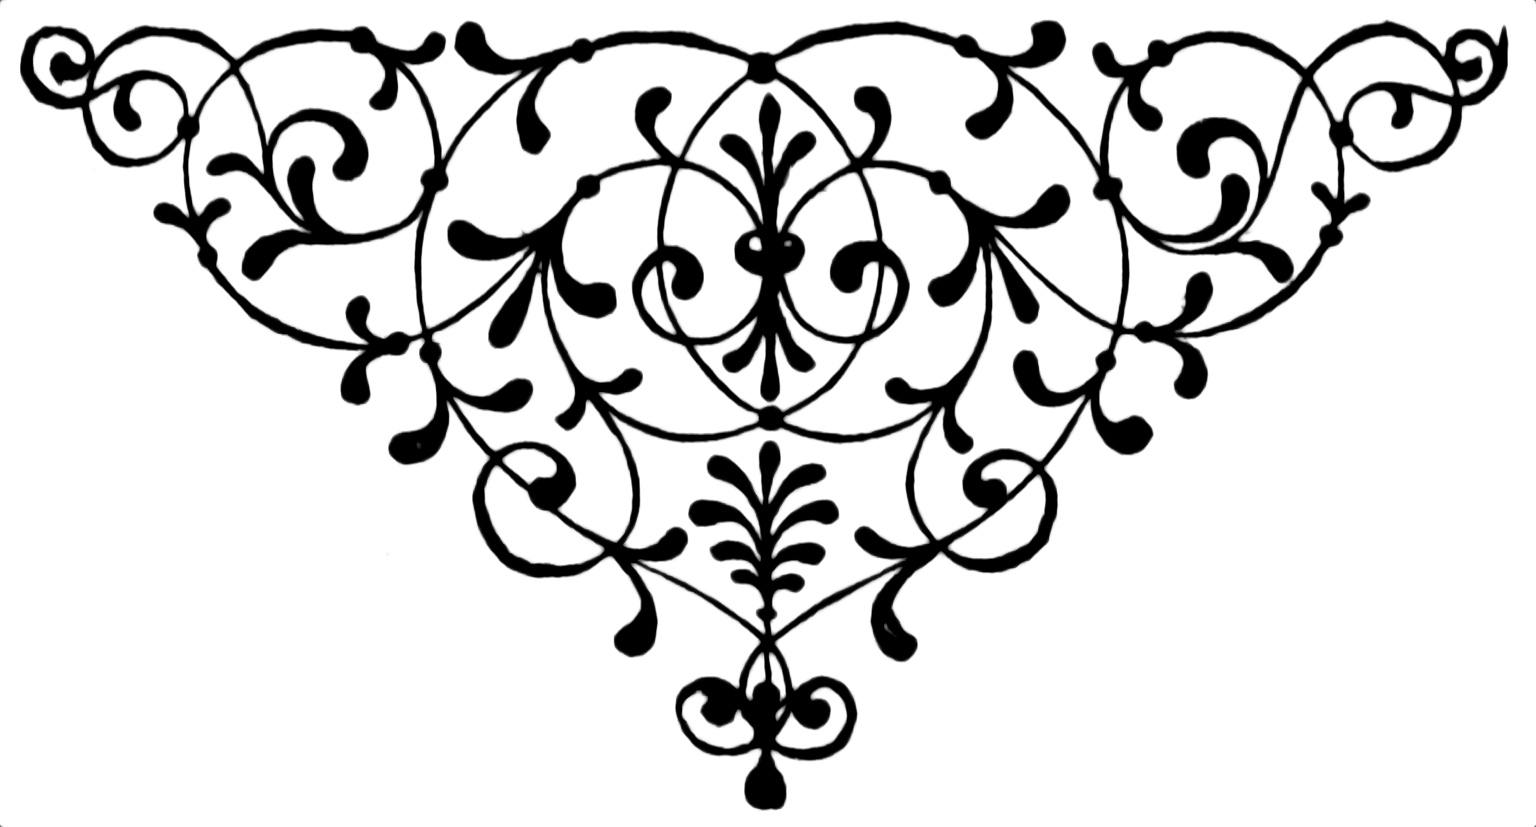
\includegraphics[width=.8\linewidth]{theend}
\end{center}



\KOMAoptions{headings=openright}
%\KOMAoptions{fontsize=12.5pt}
%\vspace*{-2.5cm}


%\cleardoublepage
\RedeclareSectionCommand[afterskip=1cm,beforeskip=0cm]{chapter}
\KOMAoptions{headings=openleft}
\chapter*{Colophon}

\centering
\begin{minipage}{\textwidth}
Frances Hodgson Burnett (1849--1924) published at least two earlier forms of this story—a short story <Sara Crewe: or, What Happened at Miss Minchin's>, which was serialised in \textit{St Nicholas Magazine} in 1887--1888; and a 1902 play \textit{A Little Un-fairy Princess}—before its 1905 publication by Charles Scribner's Sons in London (UK), under the title \textit{A Little Princess: Being the Whole Story of Sara Crewe Now Being Told for the First Time}.
\end{minipage}
\vfill
gutenberg.org/ebooks/146
\vfill
\rule{0.5\textwidth}{.4pt}
\vfill
\begin{minipage}{\textwidth}
EB Garamond is Georg Mayr-Duffner's free and open source implementation of Claude Garamond’s famous humanist typefaces from the mid-sixteenth century. 
\end{minipage}
\vfill
\begin{minipage}{\textwidth}
Title page is set in <Chelsea>, by Dieter Steffmann. Dropcaps are set in <Floral Capitals>, by Vladimir Nikolic.
\end{minipage}
\vfill
github.com/georgd/EB-Garamond\\
steffmann.de\\
coroflot.com/vladimirnikolic
\vfill
\rule{0.5\textwidth}{.4pt}
\vfill
\begin{minipage}{\textwidth}
Title page decoration is by the Gatchell \& Manning engraving firm of Philadelphia (USA), and was originally published in \textit{The Inland Printer} in 1919. Last page decoration and chapter head decorations are taken from \textit{Wark's Modern Educator}, published by Henry Wark in New York (USA) in 1904.
\end{minipage}
\vfill
\rule{0.5\textwidth}{.4pt}
\vfill
\begin{minipage}{\textwidth}
This typeset is dedicated to the public domain under a Creative Commons CC0 1.0 Universal deed.\end{minipage}
\vfill
creativecommons.org/publicdomain/zero/1.0/
\vfill
\rule{0.5\textwidth}{.4pt}
\vfill
Typeset in \LaTeX{}. Last revised \today.
\thispagestyle{empty}


\end{document}